\documentclass[twoside]{book}

% Packages required by doxygen
\usepackage{fixltx2e}
\usepackage{calc}
\usepackage{doxygen}
\usepackage[export]{adjustbox} % also loads graphicx
\usepackage{graphicx}
\usepackage[utf8]{inputenc}
\usepackage{makeidx}
\usepackage{multicol}
\usepackage{multirow}
\PassOptionsToPackage{warn}{textcomp}
\usepackage{textcomp}
\usepackage[nointegrals]{wasysym}
\usepackage[table]{xcolor}

% Font selection
\usepackage[T1]{fontenc}
\usepackage[scaled=.90]{helvet}
\usepackage{courier}
\usepackage{amssymb}
\usepackage{sectsty}
\renewcommand{\familydefault}{\sfdefault}
\allsectionsfont{%
  \fontseries{bc}\selectfont%
  \color{darkgray}%
}
\renewcommand{\DoxyLabelFont}{%
  \fontseries{bc}\selectfont%
  \color{darkgray}%
}
\newcommand{\+}{\discretionary{\mbox{\scriptsize$\hookleftarrow$}}{}{}}

% Page & text layout
\usepackage{geometry}
\geometry{%
  a4paper,%
  top=2.5cm,%
  bottom=2.5cm,%
  left=2.5cm,%
  right=2.5cm%
}
\tolerance=750
\hfuzz=15pt
\hbadness=750
\setlength{\emergencystretch}{15pt}
\setlength{\parindent}{0cm}
\setlength{\parskip}{3ex plus 2ex minus 2ex}
\makeatletter
\renewcommand{\paragraph}{%
  \@startsection{paragraph}{4}{0ex}{-1.0ex}{1.0ex}{%
    \normalfont\normalsize\bfseries\SS@parafont%
  }%
}
\renewcommand{\subparagraph}{%
  \@startsection{subparagraph}{5}{0ex}{-1.0ex}{1.0ex}{%
    \normalfont\normalsize\bfseries\SS@subparafont%
  }%
}
\makeatother

% Headers & footers
\usepackage{fancyhdr}
\pagestyle{fancyplain}
\fancyhead[LE]{\fancyplain{}{\bfseries\thepage}}
\fancyhead[CE]{\fancyplain{}{}}
\fancyhead[RE]{\fancyplain{}{\bfseries\leftmark}}
\fancyhead[LO]{\fancyplain{}{\bfseries\rightmark}}
\fancyhead[CO]{\fancyplain{}{}}
\fancyhead[RO]{\fancyplain{}{\bfseries\thepage}}
\fancyfoot[LE]{\fancyplain{}{}}
\fancyfoot[CE]{\fancyplain{}{}}
\fancyfoot[RE]{\fancyplain{}{\bfseries\scriptsize Generated by Doxygen }}
\fancyfoot[LO]{\fancyplain{}{\bfseries\scriptsize Generated by Doxygen }}
\fancyfoot[CO]{\fancyplain{}{}}
\fancyfoot[RO]{\fancyplain{}{}}
\renewcommand{\footrulewidth}{0.4pt}
\renewcommand{\chaptermark}[1]{%
  \markboth{#1}{}%
}
\renewcommand{\sectionmark}[1]{%
  \markright{\thesection\ #1}%
}

% Indices & bibliography
\usepackage{natbib}
\usepackage[titles]{tocloft}
\setcounter{tocdepth}{3}
\setcounter{secnumdepth}{5}
\makeindex

% Hyperlinks (required, but should be loaded last)
\usepackage{ifpdf}
\ifpdf
  \usepackage[pdftex,pagebackref=true]{hyperref}
\else
  \usepackage[ps2pdf,pagebackref=true]{hyperref}
\fi
\hypersetup{%
  colorlinks=true,%
  linkcolor=blue,%
  citecolor=blue,%
  unicode%
}

% Custom commands
\newcommand{\clearemptydoublepage}{%
  \newpage{\pagestyle{empty}\cleardoublepage}%
}

\usepackage{caption}
\captionsetup{labelsep=space,justification=centering,font={bf},singlelinecheck=off,skip=4pt,position=top}

%===== C O N T E N T S =====

\begin{document}

% Titlepage & ToC
\hypersetup{pageanchor=false,
             bookmarksnumbered=true,
             pdfencoding=unicode
            }
\pagenumbering{alph}
\begin{titlepage}
\vspace*{7cm}
\begin{center}%
{\Large Pluri\+Notes \\[1ex]\large 1.\+0 }\\
\vspace*{1cm}
{\large Generated by Doxygen 1.8.13}\\
\end{center}
\end{titlepage}
\clearemptydoublepage
\pagenumbering{roman}
\tableofcontents
\clearemptydoublepage
\pagenumbering{arabic}
\hypersetup{pageanchor=true}

%--- Begin generated contents ---
\chapter{Pluri\+Notes}
\label{md__r_e_a_d_m_e}
\Hypertarget{md__r_e_a_d_m_e}
\subsection*{\hyperlink{class_note}{Note} manager project}
\chapter{Hierarchical Index}
\section{Class Hierarchy}
This inheritance list is sorted roughly, but not completely, alphabetically\+:\begin{DoxyCompactList}
\item \contentsline{section}{Centre\+Relations\+Details}{\pageref{class_centre_relations_details}}{}
\item \contentsline{section}{Couple}{\pageref{class_couple}}{}
\item \contentsline{section}{Exception}{\pageref{class_exception}}{}
\item \contentsline{section}{Iterator$<$ T $>$}{\pageref{class_iterator}}{}
\item \contentsline{section}{Iterator$<$ Couple $>$}{\pageref{class_iterator}}{}
\begin{DoxyCompactList}
\item \contentsline{section}{Relation\+:\+:iterator}{\pageref{class_relation_1_1iterator}}{}
\end{DoxyCompactList}
\item \contentsline{section}{Iterator$<$ Note $>$}{\pageref{class_iterator}}{}
\begin{DoxyCompactList}
\item \contentsline{section}{Notes\+Manager\+:\+:iterator}{\pageref{class_notes_manager_1_1iterator}}{}
\end{DoxyCompactList}
\item \contentsline{section}{Iterator$<$ Relation $>$}{\pageref{class_iterator}}{}
\begin{DoxyCompactList}
\item \contentsline{section}{Relation\+Manager\+:\+:iterator}{\pageref{class_relation_manager_1_1iterator}}{}
\end{DoxyCompactList}
\item \contentsline{section}{Iterator$<$ Version $>$}{\pageref{class_iterator}}{}
\begin{DoxyCompactList}
\item \contentsline{section}{Note\+:\+:iterator}{\pageref{class_note_1_1iterator}}{}
\end{DoxyCompactList}
\item \contentsline{section}{Note}{\pageref{class_note}}{}
\item \contentsline{section}{Notes\+Manager}{\pageref{class_notes_manager}}{}
\item Q\+Main\+Window\begin{DoxyCompactList}
\item \contentsline{section}{Interface}{\pageref{class_interface}}{}
\end{DoxyCompactList}
\item Q\+Widget\begin{DoxyCompactList}
\item \contentsline{section}{Centre\+Note\+Act}{\pageref{class_centre_note_act}}{}
\item \contentsline{section}{Centre\+Note\+Arch}{\pageref{class_centre_note_arch}}{}
\item \contentsline{section}{Centre\+Relation\+Details}{\pageref{class_centre_relation_details}}{}
\item \contentsline{section}{Centre\+Relations}{\pageref{class_centre_relations}}{}
\item \contentsline{section}{Droite\+Arborescence}{\pageref{class_droite_arborescence}}{}
\item \contentsline{section}{Gauche}{\pageref{class_gauche}}{}
\item \contentsline{section}{Window\+Afficher\+Article}{\pageref{class_window_afficher_article}}{}
\item \contentsline{section}{Window\+Afficher\+Audio}{\pageref{class_window_afficher_audio}}{}
\item \contentsline{section}{Window\+Afficher\+Couple}{\pageref{class_window_afficher_couple}}{}
\item \contentsline{section}{Window\+Afficher\+Image}{\pageref{class_window_afficher_image}}{}
\item \contentsline{section}{Window\+Afficher\+Tache}{\pageref{class_window_afficher_tache}}{}
\item \contentsline{section}{Window\+Afficher\+Video}{\pageref{class_window_afficher_video}}{}
\item \contentsline{section}{Window\+Creer\+Article}{\pageref{class_window_creer_article}}{}
\item \contentsline{section}{Window\+Creer\+Audio}{\pageref{class_window_creer_audio}}{}
\item \contentsline{section}{Window\+Creer\+Couple}{\pageref{class_window_creer_couple}}{}
\item \contentsline{section}{Window\+Creer\+Image}{\pageref{class_window_creer_image}}{}
\item \contentsline{section}{Window\+Creer\+Note}{\pageref{class_window_creer_note}}{}
\item \contentsline{section}{Window\+Creer\+Relation}{\pageref{class_window_creer_relation}}{}
\item \contentsline{section}{Window\+Creer\+Tache}{\pageref{class_window_creer_tache}}{}
\item \contentsline{section}{Window\+Creer\+Video}{\pageref{class_window_creer_video}}{}
\end{DoxyCompactList}
\item \contentsline{section}{Relation}{\pageref{class_relation}}{}
\begin{DoxyCompactList}
\item \contentsline{section}{Relation\+Normale}{\pageref{class_relation_normale}}{}
\item \contentsline{section}{Relation\+Preexistente}{\pageref{class_relation_preexistente}}{}
\end{DoxyCompactList}
\item \contentsline{section}{Relation\+Manager}{\pageref{class_relation_manager}}{}
\item \contentsline{section}{Template}{\pageref{class_template}}{}
\item \contentsline{section}{Template}{\pageref{class_template}}{}
\item \contentsline{section}{Version}{\pageref{class_version}}{}
\begin{DoxyCompactList}
\item \contentsline{section}{Article}{\pageref{class_article}}{}
\item \contentsline{section}{Multimedia}{\pageref{class_multimedia}}{}
\begin{DoxyCompactList}
\item \contentsline{section}{audio}{\pageref{classaudio}}{}
\item \contentsline{section}{image}{\pageref{classimage}}{}
\item \contentsline{section}{video}{\pageref{classvideo}}{}
\end{DoxyCompactList}
\item \contentsline{section}{Tache}{\pageref{class_tache}}{}
\end{DoxyCompactList}
\item \contentsline{section}{Windowd\+Creer\+Image}{\pageref{class_windowd_creer_image}}{}
\item \contentsline{section}{Windowd\+Creer\+Note}{\pageref{class_windowd_creer_note}}{}
\item \contentsline{section}{Windowd\+Creer\+Tache}{\pageref{class_windowd_creer_tache}}{}
\item \contentsline{section}{Windowd\+Creer\+Video}{\pageref{class_windowd_creer_video}}{}
\end{DoxyCompactList}

\chapter{Class Index}
\section{Class List}
Here are the classes, structs, unions and interfaces with brief descriptions\+:\begin{DoxyCompactList}
\item\contentsline{section}{\hyperlink{class_article}{Article} \\*Définit la classe \hyperlink{class_article}{Article} }{\pageref{class_article}}{}
\item\contentsline{section}{\hyperlink{classaudio}{audio} \\*Classe audio hérite de \hyperlink{class_multimedia}{Multimedia} }{\pageref{classaudio}}{}
\item\contentsline{section}{\hyperlink{class_centre_note_act}{Centre\+Note\+Act} }{\pageref{class_centre_note_act}}{}
\item\contentsline{section}{\hyperlink{class_centre_note_arch}{Centre\+Note\+Arch} \\*Définit la classe \hyperlink{class_centre_note_arch}{Centre\+Note\+Arch} \+: Affiche les versions d\textquotesingle{}une note archivée }{\pageref{class_centre_note_arch}}{}
\item\contentsline{section}{\hyperlink{class_centre_relation_details}{Centre\+Relation\+Details} }{\pageref{class_centre_relation_details}}{}
\item\contentsline{section}{\hyperlink{class_centre_relations}{Centre\+Relations} \\*Définit la classe \hyperlink{class_centre_relations}{Centre\+Relations} \+: Gestion des relations }{\pageref{class_centre_relations}}{}
\item\contentsline{section}{\hyperlink{class_centre_relations_details}{Centre\+Relations\+Details} \\*Définit la classe \hyperlink{class_centre_relation_details}{Centre\+Relation\+Details} \+: Gestion d\textquotesingle{}une relation en particulière }{\pageref{class_centre_relations_details}}{}
\item\contentsline{section}{\hyperlink{class_couple}{Couple} \\*The \hyperlink{class_couple}{Couple} class\+: contain 2 note linked together by a relation, with label }{\pageref{class_couple}}{}
\item\contentsline{section}{\hyperlink{class_droite_arborescence}{Droite\+Arborescence} \\*The \hyperlink{class_droite_arborescence}{Droite\+Arborescence} class\+: Widget to view arborescence }{\pageref{class_droite_arborescence}}{}
\item\contentsline{section}{\hyperlink{class_exception}{Exception} \\*The \hyperlink{class_exception}{Exception} class\+: class \hyperlink{class_exception}{Exception} }{\pageref{class_exception}}{}
\item\contentsline{section}{\hyperlink{class_gauche}{Gauche} \\*Définit la classe \hyperlink{class_gauche}{Gauche} \+: Affichage des notes actives et archivées }{\pageref{class_gauche}}{}
\item\contentsline{section}{\hyperlink{classimage}{image} \\*Classe image hérite de \hyperlink{class_multimedia}{Multimedia} }{\pageref{classimage}}{}
\item\contentsline{section}{\hyperlink{class_interface}{Interface} \\*The \hyperlink{class_interface}{Interface} class\+: heritate Q\+Main\+Window, this class is Main\+Window of the program }{\pageref{class_interface}}{}
\item\contentsline{section}{\hyperlink{class_relation_1_1iterator}{Relation\+::iterator} \\*The iterator class\+: iterator of relation, iterate throught the table of couple }{\pageref{class_relation_1_1iterator}}{}
\item\contentsline{section}{\hyperlink{class_iterator}{Iterator$<$ T $>$} }{\pageref{class_iterator}}{}
\item\contentsline{section}{\hyperlink{class_relation_manager_1_1iterator}{Relation\+Manager\+::iterator} \\*The iterator class\+: iterator through table of relations }{\pageref{class_relation_manager_1_1iterator}}{}
\item\contentsline{section}{\hyperlink{class_note_1_1iterator}{Note\+::iterator} }{\pageref{class_note_1_1iterator}}{}
\item\contentsline{section}{\hyperlink{class_notes_manager_1_1iterator}{Notes\+Manager\+::iterator} }{\pageref{class_notes_manager_1_1iterator}}{}
\item\contentsline{section}{\hyperlink{class_multimedia}{Multimedia} \\*Définit la classe \hyperlink{class_multimedia}{Multimedia} et ses classes filles (image, audio, video) }{\pageref{class_multimedia}}{}
\item\contentsline{section}{\hyperlink{class_note}{Note} \\*Définit la classe Notes \+: Permet de d\textquotesingle{}ajouter, supprimer, restaurer une \hyperlink{class_version}{Version} à une \hyperlink{class_note}{Note} }{\pageref{class_note}}{}
\item\contentsline{section}{\hyperlink{class_notes_manager}{Notes\+Manager} \\*Définit la classe \hyperlink{class_notes_manager}{Notes\+Manager} \+: Permet de d\textquotesingle{}ajouter, supprimer, restaurer une \hyperlink{class_note}{Note}. Permet de sauvegarder/charger la session dans/à partir d\textquotesingle{}un fichier X\+ML }{\pageref{class_notes_manager}}{}
\item\contentsline{section}{\hyperlink{class_relation}{Relation} \\*Abstract, it contains couples and the orientation of the couples inside }{\pageref{class_relation}}{}
\item\contentsline{section}{\hyperlink{class_relation_manager}{Relation\+Manager} \\*The \hyperlink{class_relation_manager}{Relation\+Manager} class\+: \hyperlink{class_relation}{Relation} Manager to manage \hyperlink{class_relation}{Relation}, Singleton }{\pageref{class_relation_manager}}{}
\item\contentsline{section}{\hyperlink{class_relation_normale}{Relation\+Normale} \\*The \hyperlink{class_relation_normale}{Relation\+Normale} class\+: heritate of \hyperlink{class_relation}{Relation} class }{\pageref{class_relation_normale}}{}
\item\contentsline{section}{\hyperlink{class_relation_preexistente}{Relation\+Preexistente} \\*The \hyperlink{class_relation_preexistente}{Relation\+Preexistente} class\+: the Preexistence class, Reference }{\pageref{class_relation_preexistente}}{}
\item\contentsline{section}{\hyperlink{class_tache}{Tache} \\*Définit la classe \hyperlink{class_tache}{Tache} }{\pageref{class_tache}}{}
\item\contentsline{section}{\hyperlink{class_template}{Template} }{\pageref{class_template}}{}
\item\contentsline{section}{\hyperlink{class_template}{Template} }{\pageref{class_template}}{}
\item\contentsline{section}{\hyperlink{class_version}{Version} \\*Définit la classe \hyperlink{class_version}{Version} }{\pageref{class_version}}{}
\item\contentsline{section}{\hyperlink{classvideo}{video} \\*Classe video hérite de \hyperlink{class_multimedia}{Multimedia} }{\pageref{classvideo}}{}
\item\contentsline{section}{\hyperlink{class_window_afficher_article}{Window\+Afficher\+Article} \\*The \hyperlink{class_window_afficher_article}{Window\+Afficher\+Article} class\+: Widget to view and edit article }{\pageref{class_window_afficher_article}}{}
\item\contentsline{section}{\hyperlink{class_window_afficher_audio}{Window\+Afficher\+Audio} \\*Définit la classe \hyperlink{class_window_afficher_audio}{Window\+Afficher\+Audio} \+: Emplacement pour afficher un audio }{\pageref{class_window_afficher_audio}}{}
\item\contentsline{section}{\hyperlink{class_window_afficher_couple}{Window\+Afficher\+Couple} \\*The \hyperlink{class_window_afficher_couple}{Window\+Afficher\+Couple} class\+: the Widget to view all couplees of a relation }{\pageref{class_window_afficher_couple}}{}
\item\contentsline{section}{\hyperlink{class_window_afficher_image}{Window\+Afficher\+Image} \\*The Window\+Afficher\+Imag class\+: Widget to view and edit image }{\pageref{class_window_afficher_image}}{}
\item\contentsline{section}{\hyperlink{class_window_afficher_tache}{Window\+Afficher\+Tache} }{\pageref{class_window_afficher_tache}}{}
\item\contentsline{section}{\hyperlink{class_window_afficher_video}{Window\+Afficher\+Video} \\*Définit la classe \hyperlink{class_window_afficher_video}{Window\+Afficher\+Video} \+: Emplacement pour afficher un video }{\pageref{class_window_afficher_video}}{}
\item\contentsline{section}{\hyperlink{class_window_creer_article}{Window\+Creer\+Article} \\*The \hyperlink{class_window_creer_article}{Window\+Creer\+Article} class\+: Widget to create new article }{\pageref{class_window_creer_article}}{}
\item\contentsline{section}{\hyperlink{class_window_creer_audio}{Window\+Creer\+Audio} \\*The \hyperlink{class_window_creer_audio}{Window\+Creer\+Audio} class\+: Widget to create new audio }{\pageref{class_window_creer_audio}}{}
\item\contentsline{section}{\hyperlink{class_window_creer_couple}{Window\+Creer\+Couple} \\*Définit la classe \hyperlink{class_window_creer_couple}{Window\+Creer\+Couple} \+: Emplacement pour créer une couple }{\pageref{class_window_creer_couple}}{}
\item\contentsline{section}{\hyperlink{class_window_creer_image}{Window\+Creer\+Image} }{\pageref{class_window_creer_image}}{}
\item\contentsline{section}{\hyperlink{class_window_creer_note}{Window\+Creer\+Note} }{\pageref{class_window_creer_note}}{}
\item\contentsline{section}{\hyperlink{class_window_creer_relation}{Window\+Creer\+Relation} \\*Définit la classe \hyperlink{class_window_creer_relation}{Window\+Creer\+Relation} \+: Emplacement pour créer une relation }{\pageref{class_window_creer_relation}}{}
\item\contentsline{section}{\hyperlink{class_window_creer_tache}{Window\+Creer\+Tache} }{\pageref{class_window_creer_tache}}{}
\item\contentsline{section}{\hyperlink{class_window_creer_video}{Window\+Creer\+Video} }{\pageref{class_window_creer_video}}{}
\item\contentsline{section}{\hyperlink{class_windowd_creer_image}{Windowd\+Creer\+Image} \\*Définit la classe \hyperlink{class_windowd_creer_image}{Windowd\+Creer\+Image} \+: Emplacement pour la création d\textquotesingle{}une note image }{\pageref{class_windowd_creer_image}}{}
\item\contentsline{section}{\hyperlink{class_windowd_creer_note}{Windowd\+Creer\+Note} \\*Définit la classe \hyperlink{class_windowd_creer_note}{Windowd\+Creer\+Note}\+: Emplacement pour la création d\textquotesingle{}une note }{\pageref{class_windowd_creer_note}}{}
\item\contentsline{section}{\hyperlink{class_windowd_creer_tache}{Windowd\+Creer\+Tache} \\*Définit la classe \hyperlink{class_windowd_creer_tache}{Windowd\+Creer\+Tache} \+: Emplacement pour la création d\textquotesingle{}une note tâche }{\pageref{class_windowd_creer_tache}}{}
\item\contentsline{section}{\hyperlink{class_windowd_creer_video}{Windowd\+Creer\+Video} \\*Définit la classe \hyperlink{class_windowd_creer_video}{Windowd\+Creer\+Video} \+: Emplacement pour la création d\textquotesingle{}une note vidéo }{\pageref{class_windowd_creer_video}}{}
\end{DoxyCompactList}

\chapter{File Index}
\section{File List}
Here is a list of all documented files with brief descriptions\+:\begin{DoxyCompactList}
\item\contentsline{section}{\hyperlink{article_8h}{article.\+h} }{\pageref{article_8h}}{}
\item\contentsline{section}{\hyperlink{exception_8h}{exception.\+h} \\*The exception class }{\pageref{exception_8h}}{}
\item\contentsline{section}{\hyperlink{hafficheraudio_8h}{hafficheraudio.\+h} }{\pageref{hafficheraudio_8h}}{}
\item\contentsline{section}{\hyperlink{haffichervideo_8h}{haffichervideo.\+h} }{\pageref{haffichervideo_8h}}{}
\item\contentsline{section}{\hyperlink{iterator_8h}{iterator.\+h} \\*The template of iterator }{\pageref{iterator_8h}}{}
\item\contentsline{section}{\hyperlink{multimedia_8h}{multimedia.\+h} }{\pageref{multimedia_8h}}{}
\item\contentsline{section}{\hyperlink{note_8h}{note.\+h} }{\pageref{note_8h}}{}
\item\contentsline{section}{{\bfseries noteexception.\+h} }{\pageref{noteexception_8h}}{}
\item\contentsline{section}{\hyperlink{notesmanager_8h}{notesmanager.\+h} }{\pageref{notesmanager_8h}}{}
\item\contentsline{section}{\hyperlink{relation_8h}{relation.\+h} \\*The relation file\+: contain all the description of a relation, couple and \hyperlink{class_relation}{Relation} Manager }{\pageref{relation_8h}}{}
\item\contentsline{section}{\hyperlink{tache_8h}{tache.\+h} }{\pageref{tache_8h}}{}
\item\contentsline{section}{\hyperlink{version_8h}{version.\+h} }{\pageref{version_8h}}{}
\item\contentsline{section}{\hyperlink{wafficherarticle_8h}{wafficherarticle.\+h} \\*The widget to view and edit article }{\pageref{wafficherarticle_8h}}{}
\item\contentsline{section}{\hyperlink{waffichercouple_8h}{waffichercouple.\+h} \\*The widget to view all couples of a relation }{\pageref{waffichercouple_8h}}{}
\item\contentsline{section}{\hyperlink{wafficherimage_8h}{wafficherimage.\+h} \\*The widget to view view and edit image }{\pageref{wafficherimage_8h}}{}
\item\contentsline{section}{\hyperlink{waffichertache_8h}{waffichertache.\+h} \\*The widget to view and edit tache }{\pageref{waffichertache_8h}}{}
\item\contentsline{section}{\hyperlink{warborescence_8h}{warborescence.\+h} \\*The widget to view arborescence }{\pageref{warborescence_8h}}{}
\item\contentsline{section}{\hyperlink{wcreerarticle_8h}{wcreerarticle.\+h} \\*The widget to create new article }{\pageref{wcreerarticle_8h}}{}
\item\contentsline{section}{\hyperlink{wcreeraudio_8h}{wcreeraudio.\+h} \\*The widget to create audio }{\pageref{wcreeraudio_8h}}{}
\item\contentsline{section}{{\bfseries wcreercouple.\+h} }{\pageref{wcreercouple_8h}}{}
\item\contentsline{section}{\hyperlink{wcreerimage_8h}{wcreerimage.\+h} }{\pageref{wcreerimage_8h}}{}
\item\contentsline{section}{\hyperlink{wcreernote_8h}{wcreernote.\+h} }{\pageref{wcreernote_8h}}{}
\item\contentsline{section}{\hyperlink{wcreertache_8h}{wcreertache.\+h} }{\pageref{wcreertache_8h}}{}
\item\contentsline{section}{\hyperlink{wcreervideo_8h}{wcreervideo.\+h} }{\pageref{wcreervideo_8h}}{}
\item\contentsline{section}{\hyperlink{wgauche_8h}{wgauche.\+h} }{\pageref{wgauche_8h}}{}
\item\contentsline{section}{\hyperlink{windowcreerrelation_8h}{windowcreerrelation.\+h} }{\pageref{windowcreerrelation_8h}}{}
\item\contentsline{section}{\hyperlink{winterface_8h}{winterface.\+h} \\*The main window }{\pageref{winterface_8h}}{}
\item\contentsline{section}{{\bfseries wnoteact.\+h} }{\pageref{wnoteact_8h}}{}
\item\contentsline{section}{\hyperlink{wnotearch_8h}{wnotearch.\+h} }{\pageref{wnotearch_8h}}{}
\item\contentsline{section}{{\bfseries wrelationdetails.\+h} }{\pageref{wrelationdetails_8h}}{}
\item\contentsline{section}{\hyperlink{wrelations_8h}{wrelations.\+h} }{\pageref{wrelations_8h}}{}
\end{DoxyCompactList}

\chapter{Class Documentation}
\hypertarget{class_article}{}\section{Article Class Reference}
\label{class_article}\index{Article@{Article}}


Définit la classe \hyperlink{class_article}{Article}.  




{\ttfamily \#include $<$article.\+h$>$}

Inheritance diagram for Article\+:\begin{figure}[H]
\begin{center}
\leavevmode
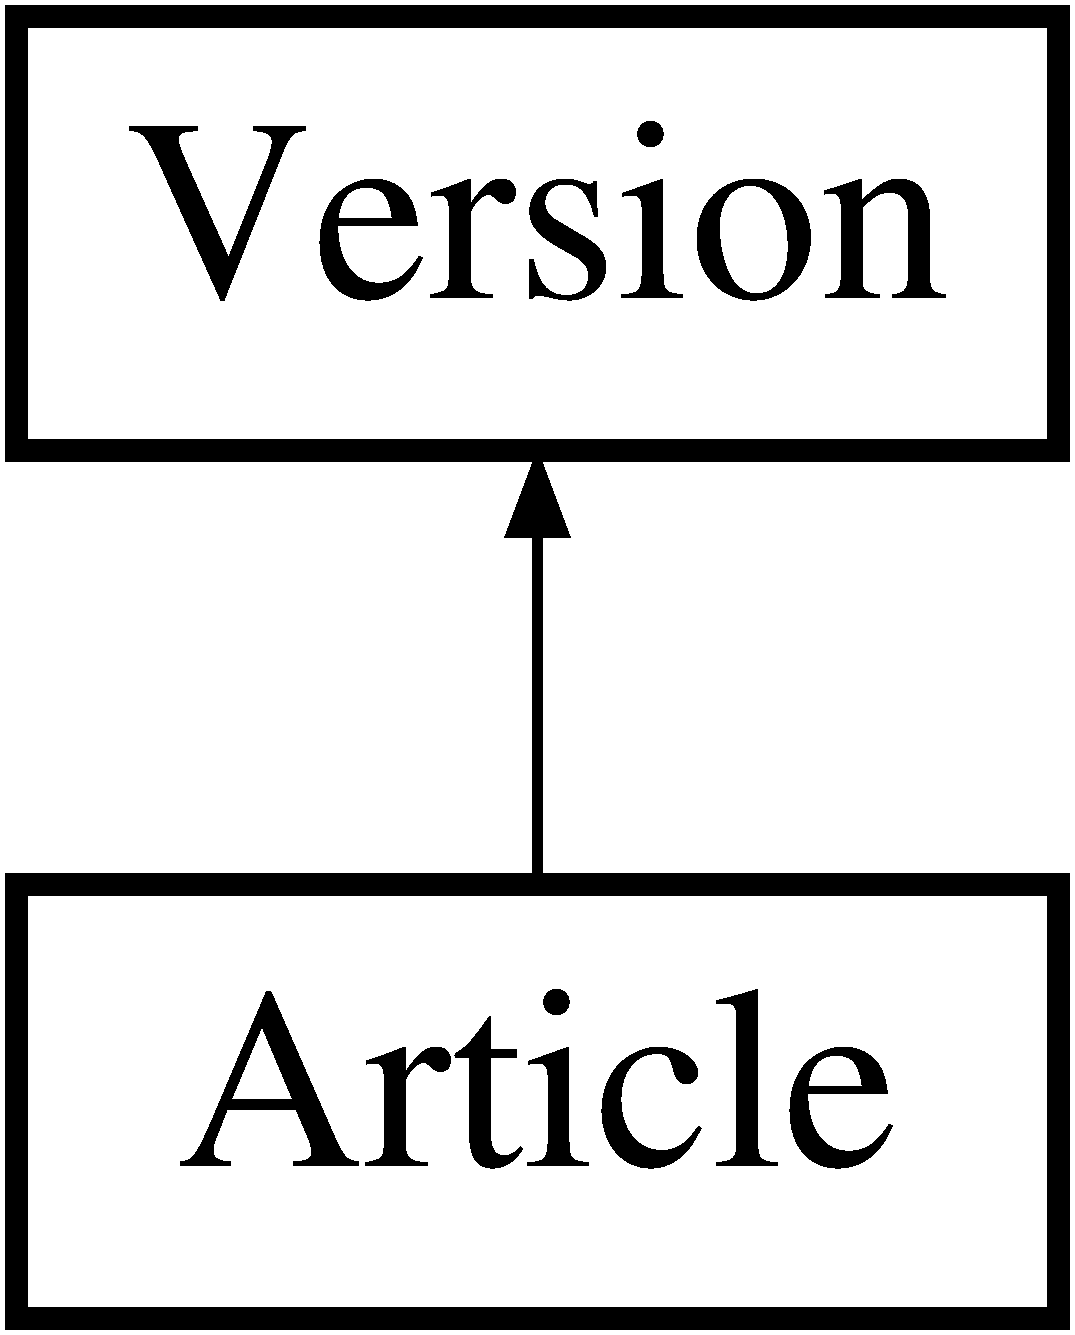
\includegraphics[height=2.000000cm]{class_article}
\end{center}
\end{figure}
\subsection*{Public Member Functions}
\begin{DoxyCompactItemize}
\item 
\mbox{\Hypertarget{class_article_aeeebcc77729439ee87c940b56524f419}\label{class_article_aeeebcc77729439ee87c940b56524f419}} 
{\bfseries Article} (const Q\+String \&t, Q\+Date\+Time d, const Q\+String \&tx)
\item 
\mbox{\Hypertarget{class_article_a235fb07dfa8507b171c35624ada564d7}\label{class_article_a235fb07dfa8507b171c35624ada564d7}} 
const Q\+String \& {\bfseries get\+Text} () const
\item 
\mbox{\Hypertarget{class_article_a6e5e9fa68313373dc0d30de3e45cd195}\label{class_article_a6e5e9fa68313373dc0d30de3e45cd195}} 
void {\bfseries set\+Text} (const Q\+String \&new\+Text)
\end{DoxyCompactItemize}


\subsection{Detailed Description}
Définit la classe \hyperlink{class_article}{Article}. 

Hérite de {\bfseries \hyperlink{class_version}{Version}} {\itshape text} \+: Texte de l\textquotesingle{}article 

The documentation for this class was generated from the following file\+:\begin{DoxyCompactItemize}
\item 
\hyperlink{article_8h}{article.\+h}\end{DoxyCompactItemize}

\hypertarget{classaudio}{}\section{audio Class Reference}
\label{classaudio}\index{audio@{audio}}


Classe audio hérite de \hyperlink{class_multimedia}{Multimedia}.  




{\ttfamily \#include $<$multimedia.\+h$>$}

Inheritance diagram for audio\+:\begin{figure}[H]
\begin{center}
\leavevmode
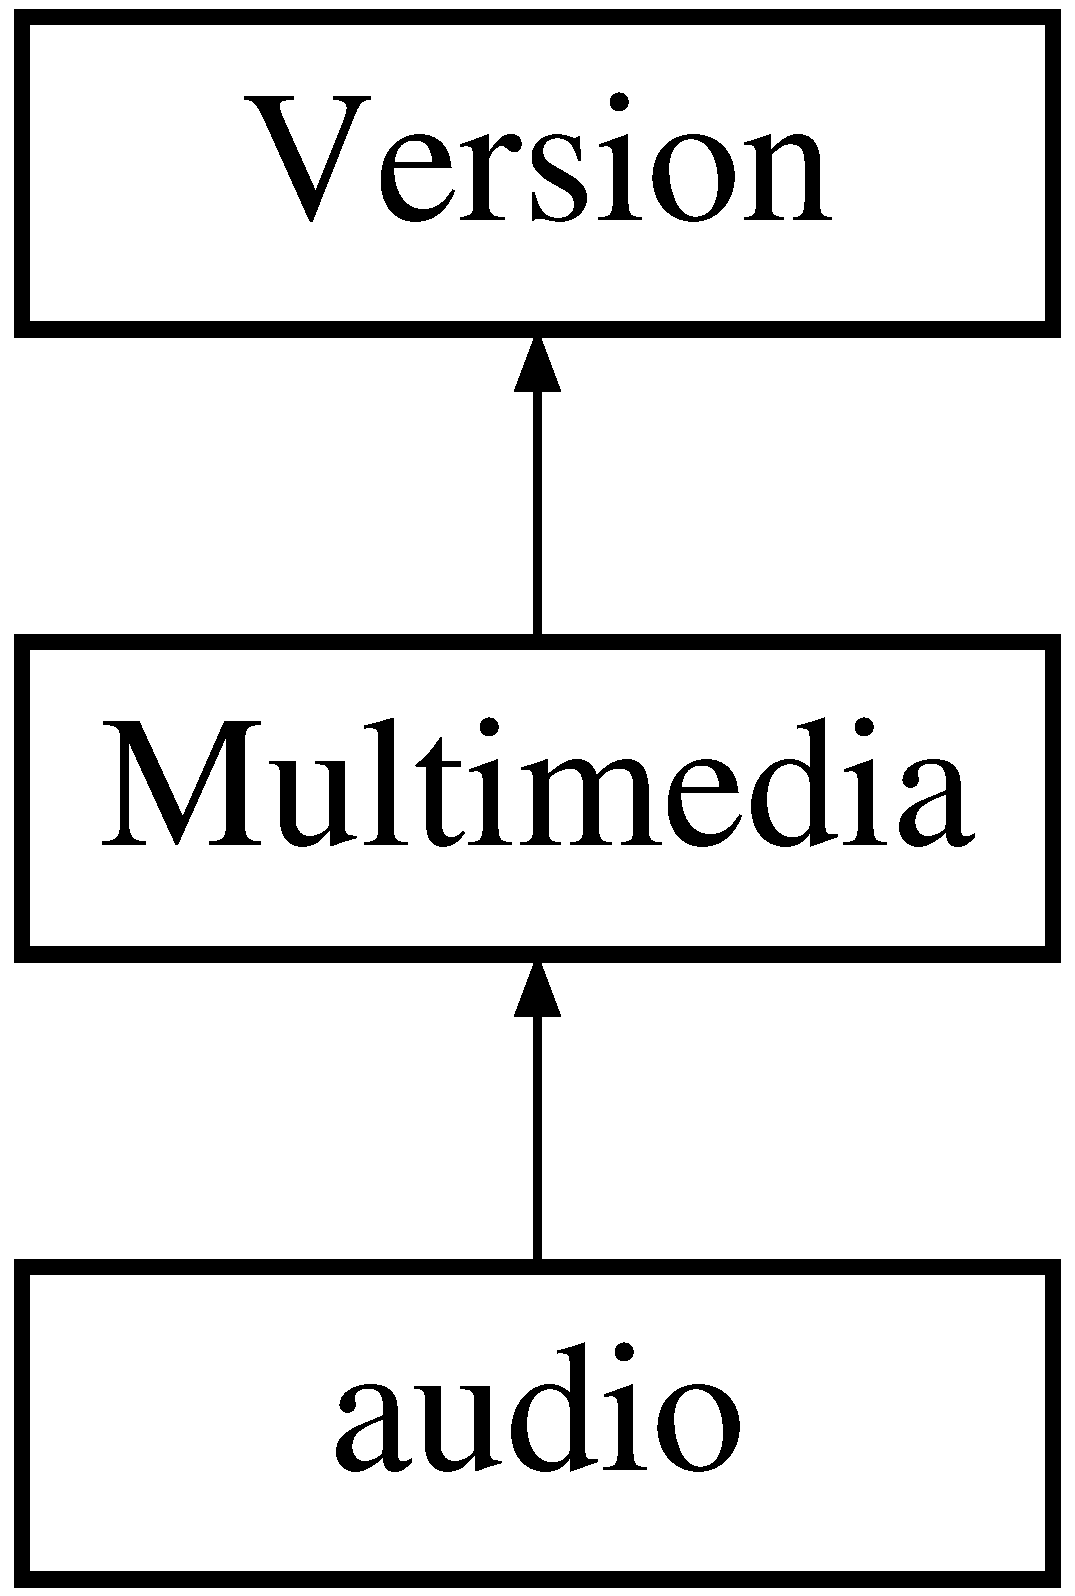
\includegraphics[height=3.000000cm]{classaudio}
\end{center}
\end{figure}
\subsection*{Public Member Functions}
\begin{DoxyCompactItemize}
\item 
\mbox{\Hypertarget{classaudio_a9e7d4c43c9e064e7f0226384d21bed05}\label{classaudio_a9e7d4c43c9e064e7f0226384d21bed05}} 
{\bfseries audio} (const Q\+String \&t, Q\+Date\+Time d, const Q\+String \&desc, const Q\+String \&i, Q\+String au)
\item 
void \hyperlink{classaudio_afa3edab5ab68f7a2b81add684b420229}{play\+Audio} () const
\item 
void \hyperlink{classaudio_a60e83448a15e15ad9807fe7bfaa1c3a6}{pause\+Audio} () const
\item 
void \hyperlink{classaudio_a0006d6803ff781ff76b8e2fda0924cd0}{stop\+Audio} () const
\item 
\mbox{\Hypertarget{classaudio_a6023815b556b82d134528ca71382c079}\label{classaudio_a6023815b556b82d134528ca71382c079}} 
const Q\+String \& {\bfseries get\+Audio\+\_\+\+U\+RL} () const
\item 
\mbox{\Hypertarget{classaudio_ab7ed38ab7898672a76c76dc53ee015b4}\label{classaudio_ab7ed38ab7898672a76c76dc53ee015b4}} 
void {\bfseries set\+Audio\+\_\+\+U\+RL} (const Q\+String \&aud\+\_\+\+U\+RL)
\end{DoxyCompactItemize}


\subsection{Detailed Description}
Classe audio hérite de \hyperlink{class_multimedia}{Multimedia}. 

\hyperlink{class_note}{Note} audio {\itshape img} \+: Q\+String lien vers le fichier audio. 

\subsection{Member Function Documentation}
\mbox{\Hypertarget{classaudio_a60e83448a15e15ad9807fe7bfaa1c3a6}\label{classaudio_a60e83448a15e15ad9807fe7bfaa1c3a6}} 
\index{audio@{audio}!pause\+Audio@{pause\+Audio}}
\index{pause\+Audio@{pause\+Audio}!audio@{audio}}
\subsubsection{\texorpdfstring{pause\+Audio()}{pauseAudio()}}
{\footnotesize\ttfamily void audio\+::pause\+Audio (\begin{DoxyParamCaption}{ }\end{DoxyParamCaption}) const}

Met en pause le fichier audio \mbox{\Hypertarget{classaudio_afa3edab5ab68f7a2b81add684b420229}\label{classaudio_afa3edab5ab68f7a2b81add684b420229}} 
\index{audio@{audio}!play\+Audio@{play\+Audio}}
\index{play\+Audio@{play\+Audio}!audio@{audio}}
\subsubsection{\texorpdfstring{play\+Audio()}{playAudio()}}
{\footnotesize\ttfamily void audio\+::play\+Audio (\begin{DoxyParamCaption}{ }\end{DoxyParamCaption}) const}

Lance le fichier audio \mbox{\Hypertarget{classaudio_a0006d6803ff781ff76b8e2fda0924cd0}\label{classaudio_a0006d6803ff781ff76b8e2fda0924cd0}} 
\index{audio@{audio}!stop\+Audio@{stop\+Audio}}
\index{stop\+Audio@{stop\+Audio}!audio@{audio}}
\subsubsection{\texorpdfstring{stop\+Audio()}{stopAudio()}}
{\footnotesize\ttfamily void audio\+::stop\+Audio (\begin{DoxyParamCaption}{ }\end{DoxyParamCaption}) const}

Stop le fichier audio en cours de lecture 

The documentation for this class was generated from the following files\+:\begin{DoxyCompactItemize}
\item 
\hyperlink{multimedia_8h}{multimedia.\+h}\item 
multimedia.\+cpp\end{DoxyCompactItemize}

\hypertarget{class_centre_note_act}{}\section{Centre\+Note\+Act Class Reference}
\label{class_centre_note_act}\index{Centre\+Note\+Act@{Centre\+Note\+Act}}
Inheritance diagram for Centre\+Note\+Act\+:\begin{figure}[H]
\begin{center}
\leavevmode
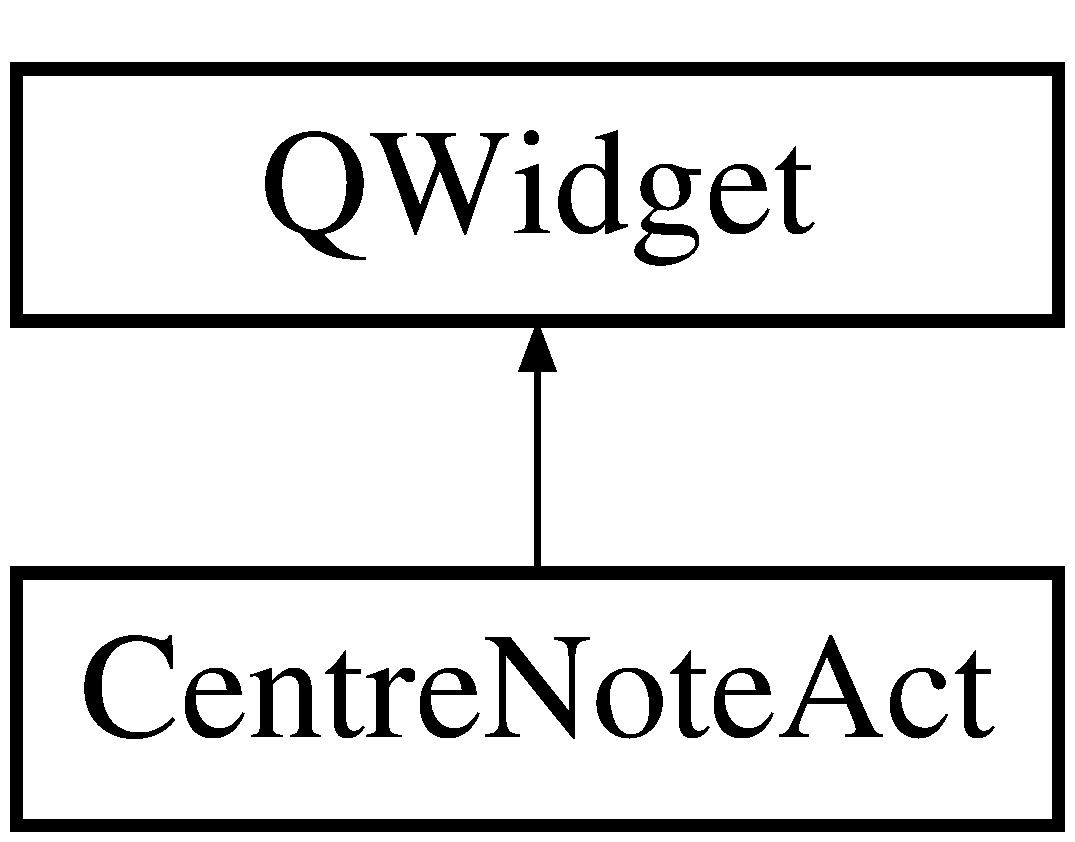
\includegraphics[height=2.000000cm]{class_centre_note_act}
\end{center}
\end{figure}
\subsection*{Public Member Functions}
\begin{DoxyCompactItemize}
\item 
\mbox{\Hypertarget{class_centre_note_act_ac77aaaac64ef24e9fb37f60113e7457c}\label{class_centre_note_act_ac77aaaac64ef24e9fb37f60113e7457c}} 
{\bfseries Centre\+Note\+Act} (\hyperlink{class_note}{Note} $\ast$it, Q\+Widget $\ast$parent=0)
\item 
\mbox{\Hypertarget{class_centre_note_act_ae4e63afb8943914798c52a0b5d2f41c8}\label{class_centre_note_act_ae4e63afb8943914798c52a0b5d2f41c8}} 
Q\+Push\+Button $\ast$ {\bfseries get\+Bouton\+Afficher\+Version} ()
\item 
\mbox{\Hypertarget{class_centre_note_act_a76122ca16510ed8a04ecf2725f9a1d16}\label{class_centre_note_act_a76122ca16510ed8a04ecf2725f9a1d16}} 
Q\+Push\+Button $\ast$ {\bfseries get\+Bouton\+Restaurer\+Version} ()
\item 
\mbox{\Hypertarget{class_centre_note_act_ab623b36f37425a8abe9e0fbad8c58503}\label{class_centre_note_act_ab623b36f37425a8abe9e0fbad8c58503}} 
Q\+List\+Widget $\ast$ {\bfseries get\+List\+Versions} ()
\end{DoxyCompactItemize}


The documentation for this class was generated from the following files\+:\begin{DoxyCompactItemize}
\item 
wnoteact.\+h\item 
wnoteact.\+cpp\end{DoxyCompactItemize}

\hypertarget{class_centre_note_arch}{}\section{Centre\+Note\+Arch Class Reference}
\label{class_centre_note_arch}\index{Centre\+Note\+Arch@{Centre\+Note\+Arch}}


Définit la classe \hyperlink{class_centre_note_arch}{Centre\+Note\+Arch} \+: Affiche les versions d\textquotesingle{}une note archivée.  




{\ttfamily \#include $<$wnotearch.\+h$>$}

Inheritance diagram for Centre\+Note\+Arch\+:\begin{figure}[H]
\begin{center}
\leavevmode
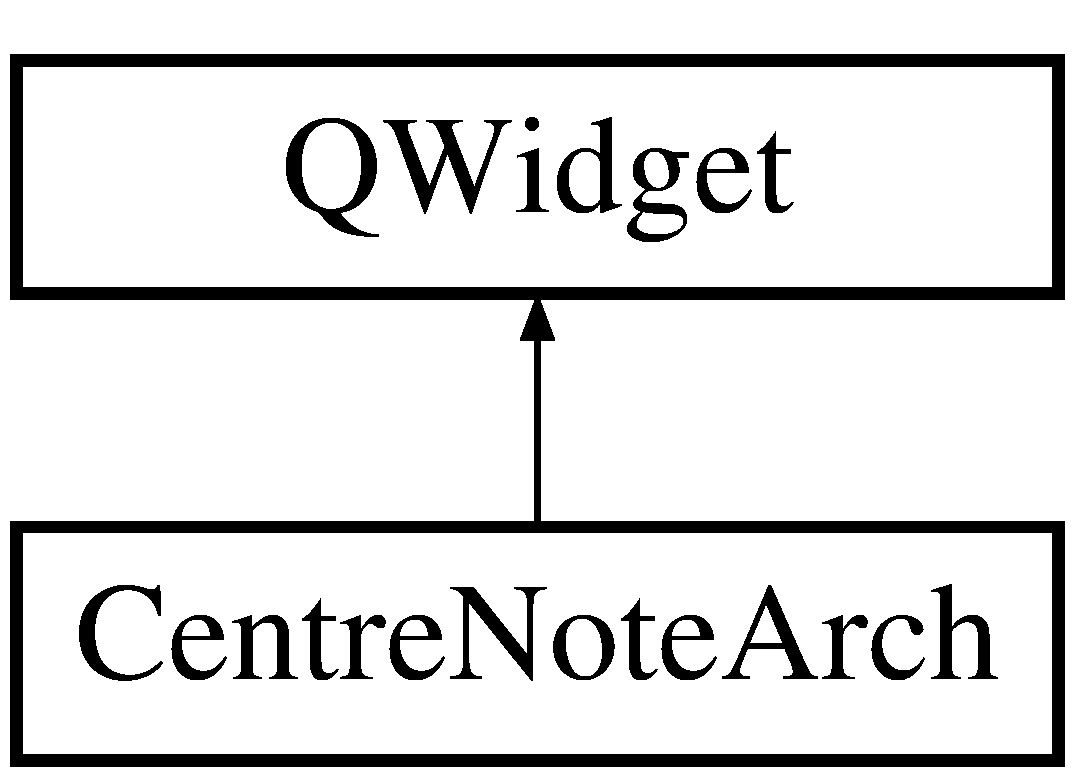
\includegraphics[height=2.000000cm]{class_centre_note_arch}
\end{center}
\end{figure}
\subsection*{Public Member Functions}
\begin{DoxyCompactItemize}
\item 
\mbox{\Hypertarget{class_centre_note_arch_a82abbbbdd856c6ce44b320491eb8c530}\label{class_centre_note_arch_a82abbbbdd856c6ce44b320491eb8c530}} 
{\bfseries Centre\+Note\+Arch} (\hyperlink{class_note}{Note} $\ast$it, Q\+Widget $\ast$parent=0)
\item 
\mbox{\Hypertarget{class_centre_note_arch_afb5b8d5f902f8ca3f0ca8f36b872638e}\label{class_centre_note_arch_afb5b8d5f902f8ca3f0ca8f36b872638e}} 
Q\+Push\+Button $\ast$ {\bfseries get\+Bouton\+Afficher\+Version} ()
\item 
\mbox{\Hypertarget{class_centre_note_arch_ab7c56ce1b22a9e95cc2b6363e30adf96}\label{class_centre_note_arch_ab7c56ce1b22a9e95cc2b6363e30adf96}} 
Q\+List\+Widget $\ast$ {\bfseries get\+List\+Versions} ()
\end{DoxyCompactItemize}


\subsection{Detailed Description}
Définit la classe \hyperlink{class_centre_note_arch}{Centre\+Note\+Arch} \+: Affiche les versions d\textquotesingle{}une note archivée. 

Hérite de Q\+Widget versions \+: Liste des versions de la note archivée afficher \+: Bouton afficher fermer \+: Bouton fermer 

The documentation for this class was generated from the following files\+:\begin{DoxyCompactItemize}
\item 
\hyperlink{wnotearch_8h}{wnotearch.\+h}\item 
wnotearch.\+cpp\end{DoxyCompactItemize}

\hypertarget{class_centre_relation_details}{}\section{Centre\+Relation\+Details Class Reference}
\label{class_centre_relation_details}\index{Centre\+Relation\+Details@{Centre\+Relation\+Details}}
Inheritance diagram for Centre\+Relation\+Details\+:\begin{figure}[H]
\begin{center}
\leavevmode
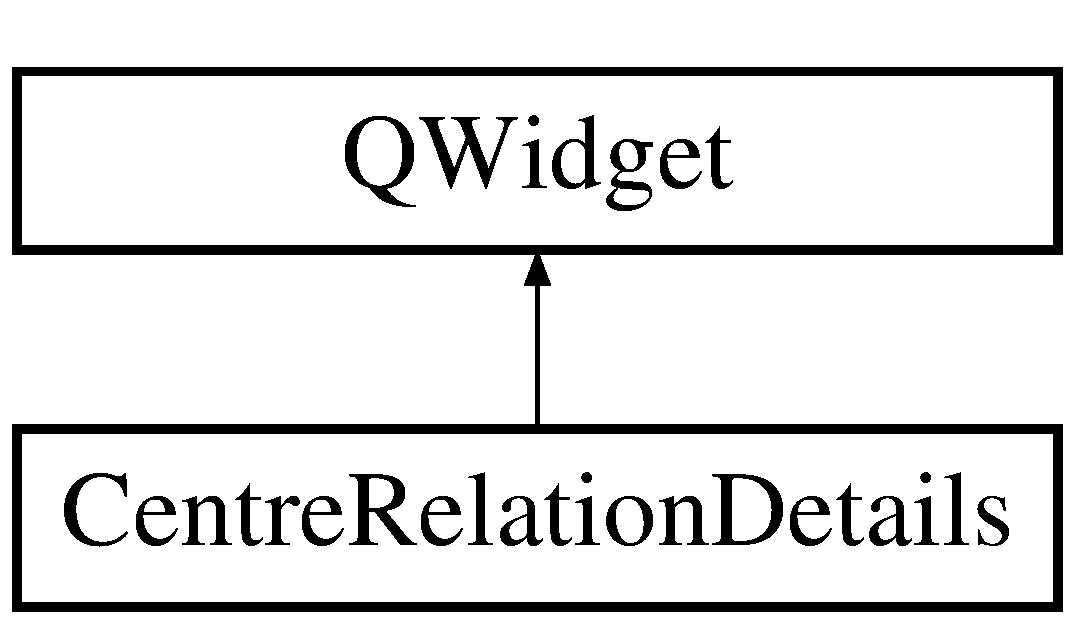
\includegraphics[height=2.000000cm]{class_centre_relation_details}
\end{center}
\end{figure}
\subsection*{Public Member Functions}
\begin{DoxyCompactItemize}
\item 
\mbox{\Hypertarget{class_centre_relation_details_ac6defcbb98de2c88728da1c260bf0b6f}\label{class_centre_relation_details_ac6defcbb98de2c88728da1c260bf0b6f}} 
{\bfseries Centre\+Relation\+Details} (\hyperlink{class_relation}{Relation} $\ast$relat, Q\+Main\+Window $\ast$parent=0)
\end{DoxyCompactItemize}


The documentation for this class was generated from the following files\+:\begin{DoxyCompactItemize}
\item 
wrelationdetails.\+h\item 
wrelationdetails.\+cpp\end{DoxyCompactItemize}

\hypertarget{class_centre_relations}{}\section{Centre\+Relations Class Reference}
\label{class_centre_relations}\index{Centre\+Relations@{Centre\+Relations}}


Définit la classe \hyperlink{class_centre_relations}{Centre\+Relations} \+: Gestion des relations.  




{\ttfamily \#include $<$wrelations.\+h$>$}

Inheritance diagram for Centre\+Relations\+:\begin{figure}[H]
\begin{center}
\leavevmode
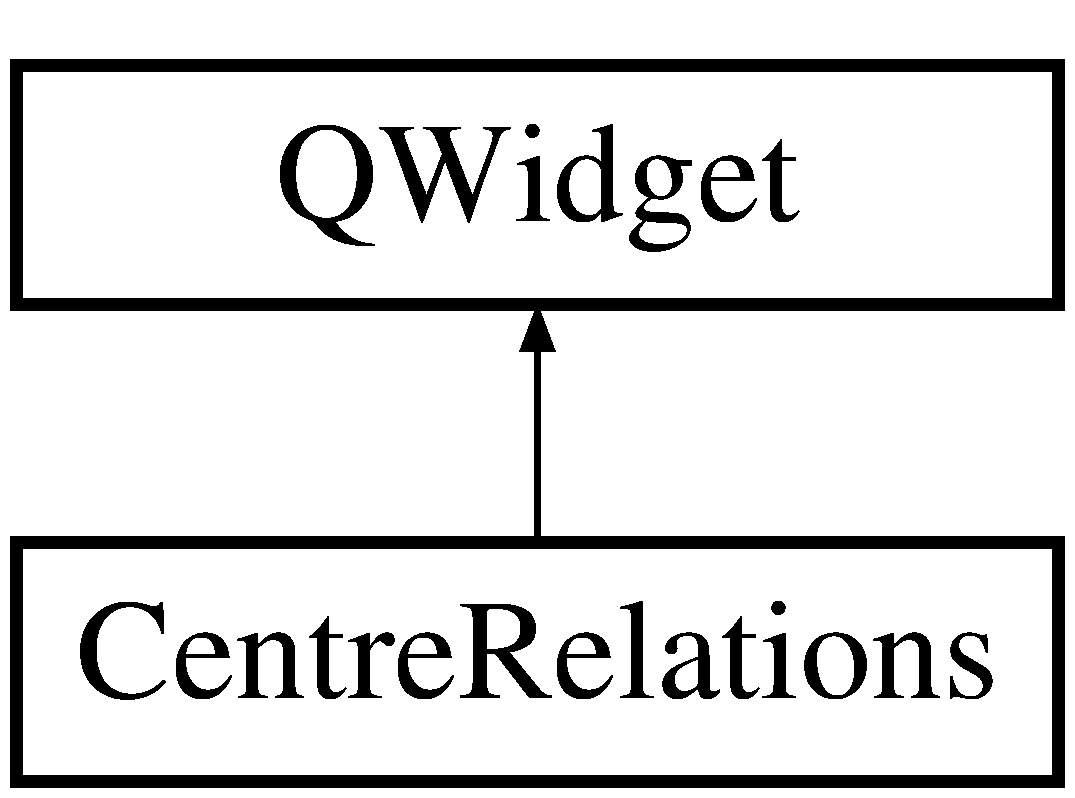
\includegraphics[height=2.000000cm]{class_centre_relations}
\end{center}
\end{figure}
\subsection*{Public Slots}
\begin{DoxyCompactItemize}
\item 
\mbox{\Hypertarget{class_centre_relations_ac8503826979abeaea33b2284196dd3a0}\label{class_centre_relations_ac8503826979abeaea33b2284196dd3a0}} 
void \hyperlink{class_centre_relations_ac8503826979abeaea33b2284196dd3a0}{supprimer\+Relation} ()
\begin{DoxyCompactList}\small\item\em Supprime une relation. \end{DoxyCompactList}\end{DoxyCompactItemize}
\subsection*{Public Member Functions}
\begin{DoxyCompactItemize}
\item 
\mbox{\Hypertarget{class_centre_relations_ad0acb1b924d26acd8d360822e79d1934}\label{class_centre_relations_ad0acb1b924d26acd8d360822e79d1934}} 
{\bfseries Centre\+Relations} (Q\+Main\+Window $\ast$parent=0)
\item 
\mbox{\Hypertarget{class_centre_relations_a479c99cac3973e895162ee046d1dc384}\label{class_centre_relations_a479c99cac3973e895162ee046d1dc384}} 
Q\+Push\+Button $\ast$ {\bfseries get\+Bouton\+Afficher} ()
\item 
\mbox{\Hypertarget{class_centre_relations_af2e962e488c16f392cd0c5b567248d1a}\label{class_centre_relations_af2e962e488c16f392cd0c5b567248d1a}} 
Q\+Push\+Button $\ast$ {\bfseries get\+Bouton\+Create} ()
\item 
\mbox{\Hypertarget{class_centre_relations_a6e4fca74ff6dfa469544172670d09039}\label{class_centre_relations_a6e4fca74ff6dfa469544172670d09039}} 
Q\+List\+Widget $\ast$ {\bfseries get\+List\+Relation} ()
\item 
\mbox{\Hypertarget{class_centre_relations_aaa277d81494895db654348e2da8acb92}\label{class_centre_relations_aaa277d81494895db654348e2da8acb92}} 
unsigned int {\bfseries get\+Indice\+Relation} ()
\end{DoxyCompactItemize}


\subsection{Detailed Description}
Définit la classe \hyperlink{class_centre_relations}{Centre\+Relations} \+: Gestion des relations. 

Hérite de Q\+Widget relations \+: Liste des relations afficher\+\_\+relation \+: Bouton afficher relation supprimer\+\_\+relation \+: Bouton supprimer relation creer\+\_\+relation \+:Bouton créer relation fermer \+: Bouton fermer 

The documentation for this class was generated from the following files\+:\begin{DoxyCompactItemize}
\item 
\hyperlink{wrelations_8h}{wrelations.\+h}\item 
wrelations.\+cpp\end{DoxyCompactItemize}

\hypertarget{class_centre_relations_details}{}\section{Centre\+Relations\+Details Class Reference}
\label{class_centre_relations_details}\index{Centre\+Relations\+Details@{Centre\+Relations\+Details}}


Définit la classe \hyperlink{class_centre_relation_details}{Centre\+Relation\+Details} \+: Gestion d\textquotesingle{}une relation en particulière.  




\subsection{Detailed Description}
Définit la classe \hyperlink{class_centre_relation_details}{Centre\+Relation\+Details} \+: Gestion d\textquotesingle{}une relation en particulière. 

Hérite de Q\+Widget titre \+: Champ titre relation desc \+: Champ description relation orientee \+: Champ orientation relation couples \+: Liste de couples d\textquotesingle{}une relation supprimer\+\_\+relation \+: Bouton supprimer relation sauver\+: Bouton sauver ajouter\+\_\+couple \+: Bouton pour ajouter couple supprimer\+\_\+couple \+: Bouton pour supprimer couple 

The documentation for this class was generated from the following file\+:\begin{DoxyCompactItemize}
\item 
wrelationdetails.\+h\end{DoxyCompactItemize}

\hypertarget{class_couple}{}\section{Couple Class Reference}
\label{class_couple}\index{Couple@{Couple}}


The \hyperlink{class_couple}{Couple} class\+: contain 2 note linked together by a relation, with label.  




{\ttfamily \#include $<$relation.\+h$>$}

\subsection*{Public Member Functions}
\begin{DoxyCompactItemize}
\item 
\hyperlink{class_couple_a8f1b8ad6f5a177161ea03b35b4af92f1}{Couple} (\hyperlink{class_note}{Note} $\ast$n1, \hyperlink{class_note}{Note} $\ast$n2, Q\+String \&lb)
\begin{DoxyCompactList}\small\item\em \hyperlink{class_couple}{Couple}\+: constructor of couple. \end{DoxyCompactList}\item 
const \hyperlink{class_note}{Note} \& \hyperlink{class_couple_ab1e111ccd47d953bce5a485a40f6e7d2}{get\+Note1} () const
\begin{DoxyCompactList}\small\item\em get\+Note1\+: get the note 1 in the couple \end{DoxyCompactList}\item 
const \hyperlink{class_note}{Note} \& \hyperlink{class_couple_ad3d28199ad0170f65c4564a910167ed6}{get\+Note2} () const
\begin{DoxyCompactList}\small\item\em get\+Note2\+: get the note 1 in the couple \end{DoxyCompactList}\item 
const Q\+String \& \hyperlink{class_couple_a0f04e0130d4d44ce39e322033d85a8df}{get\+Label} () const
\begin{DoxyCompactList}\small\item\em get\+Label\+: get the label of the couple \end{DoxyCompactList}\item 
void \hyperlink{class_couple_aed2c64b89da0544329d98eb5298d984d}{set\+Label} (Q\+String \&new\+Lb)
\begin{DoxyCompactList}\small\item\em set\+Label\+: set the new label \end{DoxyCompactList}\item 
\mbox{\Hypertarget{class_couple_adb3d0b6785dd4e5ad1fafba5d90df602}\label{class_couple_adb3d0b6785dd4e5ad1fafba5d90df602}} 
\hyperlink{class_couple_adb3d0b6785dd4e5ad1fafba5d90df602}{$\sim$\+Couple} ()
\begin{DoxyCompactList}\small\item\em destructor of couple \end{DoxyCompactList}\end{DoxyCompactItemize}


\subsection{Detailed Description}
The \hyperlink{class_couple}{Couple} class\+: contain 2 note linked together by a relation, with label. 

\subsection{Constructor \& Destructor Documentation}
\mbox{\Hypertarget{class_couple_a8f1b8ad6f5a177161ea03b35b4af92f1}\label{class_couple_a8f1b8ad6f5a177161ea03b35b4af92f1}} 
\index{Couple@{Couple}!Couple@{Couple}}
\index{Couple@{Couple}!Couple@{Couple}}
\subsubsection{\texorpdfstring{Couple()}{Couple()}}
{\footnotesize\ttfamily Couple\+::\+Couple (\begin{DoxyParamCaption}\item[{\hyperlink{class_note}{Note} $\ast$}]{n1,  }\item[{\hyperlink{class_note}{Note} $\ast$}]{n2,  }\item[{Q\+String \&}]{lb }\end{DoxyParamCaption})\hspace{0.3cm}{\ttfamily [inline]}}



\hyperlink{class_couple}{Couple}\+: constructor of couple. 


\begin{DoxyParams}{Parameters}
{\em n1} & note from \\
\hline
{\em n2} & note to \\
\hline
{\em lb} & label of the couple\\
\hline
\end{DoxyParams}
This couple indicates the relation from note 1 to note 2 if it is oriented otherwise the relation between note 1 and note 2 

\subsection{Member Function Documentation}
\mbox{\Hypertarget{class_couple_a0f04e0130d4d44ce39e322033d85a8df}\label{class_couple_a0f04e0130d4d44ce39e322033d85a8df}} 
\index{Couple@{Couple}!get\+Label@{get\+Label}}
\index{get\+Label@{get\+Label}!Couple@{Couple}}
\subsubsection{\texorpdfstring{get\+Label()}{getLabel()}}
{\footnotesize\ttfamily const Q\+String\& Couple\+::get\+Label (\begin{DoxyParamCaption}{ }\end{DoxyParamCaption}) const\hspace{0.3cm}{\ttfamily [inline]}}



get\+Label\+: get the label of the couple 

\begin{DoxyReturn}{Returns}
const Q\+String\& 
\end{DoxyReturn}
\mbox{\Hypertarget{class_couple_ab1e111ccd47d953bce5a485a40f6e7d2}\label{class_couple_ab1e111ccd47d953bce5a485a40f6e7d2}} 
\index{Couple@{Couple}!get\+Note1@{get\+Note1}}
\index{get\+Note1@{get\+Note1}!Couple@{Couple}}
\subsubsection{\texorpdfstring{get\+Note1()}{getNote1()}}
{\footnotesize\ttfamily const \hyperlink{class_note}{Note}\& Couple\+::get\+Note1 (\begin{DoxyParamCaption}{ }\end{DoxyParamCaption}) const\hspace{0.3cm}{\ttfamily [inline]}}



get\+Note1\+: get the note 1 in the couple 

\begin{DoxyReturn}{Returns}
const \hyperlink{class_note}{Note}\& 
\end{DoxyReturn}
\mbox{\Hypertarget{class_couple_ad3d28199ad0170f65c4564a910167ed6}\label{class_couple_ad3d28199ad0170f65c4564a910167ed6}} 
\index{Couple@{Couple}!get\+Note2@{get\+Note2}}
\index{get\+Note2@{get\+Note2}!Couple@{Couple}}
\subsubsection{\texorpdfstring{get\+Note2()}{getNote2()}}
{\footnotesize\ttfamily const \hyperlink{class_note}{Note}\& Couple\+::get\+Note2 (\begin{DoxyParamCaption}{ }\end{DoxyParamCaption}) const\hspace{0.3cm}{\ttfamily [inline]}}



get\+Note2\+: get the note 1 in the couple 

\begin{DoxyReturn}{Returns}
const \hyperlink{class_note}{Note}\& 
\end{DoxyReturn}
\mbox{\Hypertarget{class_couple_aed2c64b89da0544329d98eb5298d984d}\label{class_couple_aed2c64b89da0544329d98eb5298d984d}} 
\index{Couple@{Couple}!set\+Label@{set\+Label}}
\index{set\+Label@{set\+Label}!Couple@{Couple}}
\subsubsection{\texorpdfstring{set\+Label()}{setLabel()}}
{\footnotesize\ttfamily void Couple\+::set\+Label (\begin{DoxyParamCaption}\item[{Q\+String \&}]{new\+Lb }\end{DoxyParamCaption})\hspace{0.3cm}{\ttfamily [inline]}}



set\+Label\+: set the new label 


\begin{DoxyParams}{Parameters}
{\em new\+Lb} & new label \\
\hline
\end{DoxyParams}


The documentation for this class was generated from the following file\+:\begin{DoxyCompactItemize}
\item 
\hyperlink{relation_8h}{relation.\+h}\end{DoxyCompactItemize}

\hypertarget{class_droite_arborescence}{}\section{Droite\+Arborescence Class Reference}
\label{class_droite_arborescence}\index{Droite\+Arborescence@{Droite\+Arborescence}}


The \hyperlink{class_droite_arborescence}{Droite\+Arborescence} class\+: Widget to view arborescence.  




{\ttfamily \#include $<$warborescence.\+h$>$}

Inheritance diagram for Droite\+Arborescence\+:\begin{figure}[H]
\begin{center}
\leavevmode
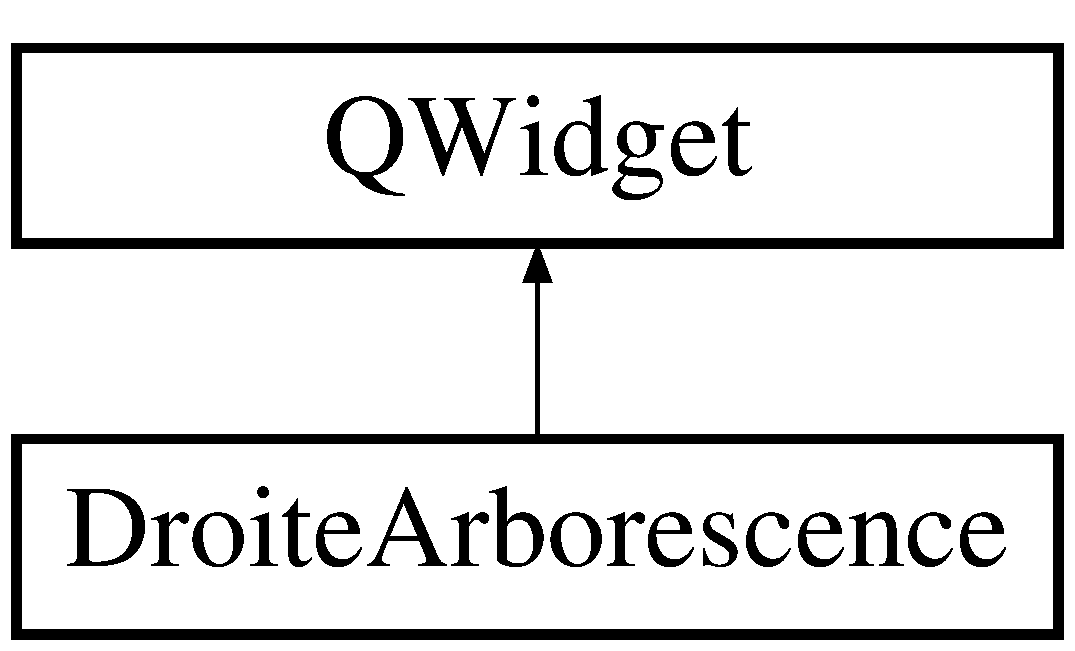
\includegraphics[height=2.000000cm]{class_droite_arborescence}
\end{center}
\end{figure}


\subsection{Detailed Description}
The \hyperlink{class_droite_arborescence}{Droite\+Arborescence} class\+: Widget to view arborescence. 

The documentation for this class was generated from the following file\+:\begin{DoxyCompactItemize}
\item 
\hyperlink{warborescence_8h}{warborescence.\+h}\end{DoxyCompactItemize}

\hypertarget{class_exception}{}\section{Exception Class Reference}
\label{class_exception}\index{Exception@{Exception}}


The \hyperlink{class_exception}{Exception} class\+: class \hyperlink{class_exception}{Exception}.  




{\ttfamily \#include $<$exception.\+h$>$}

\subsection*{Public Member Functions}
\begin{DoxyCompactItemize}
\item 
\hyperlink{class_exception_a18a14655c6ee2ab95dae815ccf1d370a}{Exception} (const Q\+String \&message)
\begin{DoxyCompactList}\small\item\em \hyperlink{class_exception}{Exception}\+: constructor of \hyperlink{class_exception}{Exception} class. \end{DoxyCompactList}\item 
Q\+String \hyperlink{class_exception_af29b1b72e34afe4a37c676200f37950b}{get\+Info} () const
\begin{DoxyCompactList}\small\item\em get\+Info\+: get error message \end{DoxyCompactList}\item 
\mbox{\Hypertarget{class_exception_a18a14655c6ee2ab95dae815ccf1d370a}\label{class_exception_a18a14655c6ee2ab95dae815ccf1d370a}} 
{\bfseries Exception} (const Q\+String \&message)
\item 
\mbox{\Hypertarget{class_exception_af29b1b72e34afe4a37c676200f37950b}\label{class_exception_af29b1b72e34afe4a37c676200f37950b}} 
Q\+String {\bfseries get\+Info} () const
\end{DoxyCompactItemize}


\subsection{Detailed Description}
The \hyperlink{class_exception}{Exception} class\+: class \hyperlink{class_exception}{Exception}. 

\subsection{Constructor \& Destructor Documentation}
\mbox{\Hypertarget{class_exception_a18a14655c6ee2ab95dae815ccf1d370a}\label{class_exception_a18a14655c6ee2ab95dae815ccf1d370a}} 
\index{Exception@{Exception}!Exception@{Exception}}
\index{Exception@{Exception}!Exception@{Exception}}
\subsubsection{\texorpdfstring{Exception()}{Exception()}}
{\footnotesize\ttfamily Exception\+::\+Exception (\begin{DoxyParamCaption}\item[{const Q\+String \&}]{message }\end{DoxyParamCaption})\hspace{0.3cm}{\ttfamily [inline]}}



\hyperlink{class_exception}{Exception}\+: constructor of \hyperlink{class_exception}{Exception} class. 


\begin{DoxyParams}{Parameters}
{\em message} & error message \\
\hline
\end{DoxyParams}


\subsection{Member Function Documentation}
\mbox{\Hypertarget{class_exception_af29b1b72e34afe4a37c676200f37950b}\label{class_exception_af29b1b72e34afe4a37c676200f37950b}} 
\index{Exception@{Exception}!get\+Info@{get\+Info}}
\index{get\+Info@{get\+Info}!Exception@{Exception}}
\subsubsection{\texorpdfstring{get\+Info()}{getInfo()}}
{\footnotesize\ttfamily Q\+String Exception\+::get\+Info (\begin{DoxyParamCaption}{ }\end{DoxyParamCaption}) const\hspace{0.3cm}{\ttfamily [inline]}}



get\+Info\+: get error message 

\begin{DoxyReturn}{Returns}
Q\+String 
\end{DoxyReturn}


The documentation for this class was generated from the following files\+:\begin{DoxyCompactItemize}
\item 
\hyperlink{exception_8h}{exception.\+h}\item 
noteexception.\+h\end{DoxyCompactItemize}

\hypertarget{class_gauche}{}\section{Gauche Class Reference}
\label{class_gauche}\index{Gauche@{Gauche}}


Définit la classe \hyperlink{class_gauche}{Gauche} \+: Affichage des notes actives et archivées.  




{\ttfamily \#include $<$wgauche.\+h$>$}

Inheritance diagram for Gauche\+:\begin{figure}[H]
\begin{center}
\leavevmode
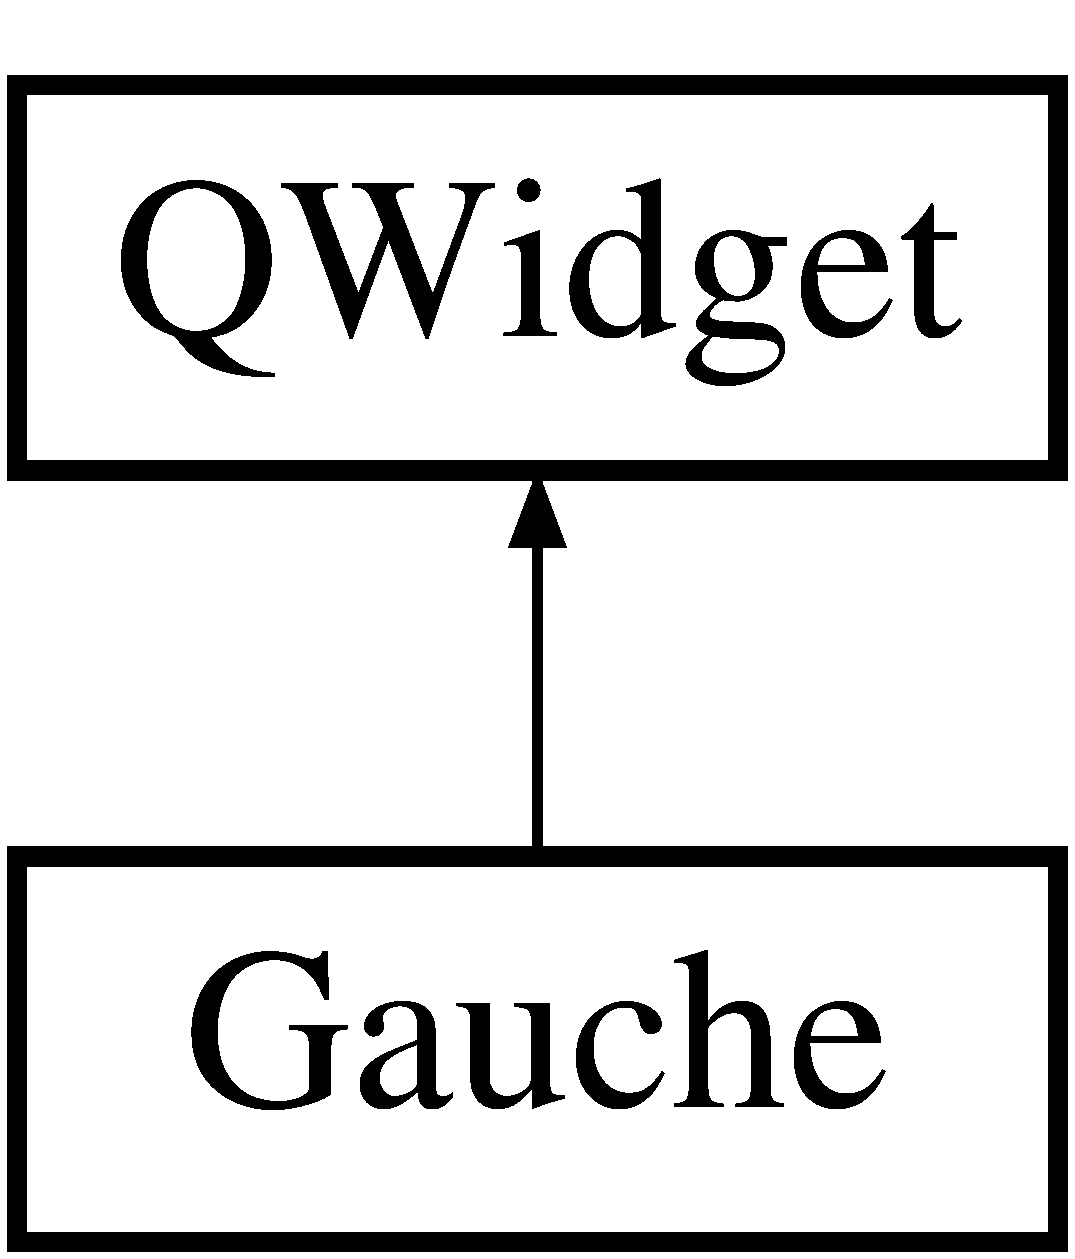
\includegraphics[height=2.000000cm]{class_gauche}
\end{center}
\end{figure}
\subsection*{Public Member Functions}
\begin{DoxyCompactItemize}
\item 
\hyperlink{class_gauche_a484580ec6e2985ffea805729dcea558e}{Gauche} (Q\+Main\+Window $\ast$parent=0)
\item 
\mbox{\Hypertarget{class_gauche_a297cbb2449edcbd05139ebd8a56982ba}\label{class_gauche_a297cbb2449edcbd05139ebd8a56982ba}} 
Q\+List\+Widget $\ast$ {\bfseries get\+Notes\+Actives} ()
\item 
\mbox{\Hypertarget{class_gauche_a2c63373c0cf72892d9cd1b30fa7f6967}\label{class_gauche_a2c63373c0cf72892d9cd1b30fa7f6967}} 
Q\+Push\+Button $\ast$ {\bfseries get\+Bouton\+Afficher\+Act} ()
\item 
\mbox{\Hypertarget{class_gauche_a027ffd7a9f33c6a72e0e729720884c69}\label{class_gauche_a027ffd7a9f33c6a72e0e729720884c69}} 
Q\+Combo\+Box $\ast$ {\bfseries get\+Notes\+Archivees} ()
\item 
\mbox{\Hypertarget{class_gauche_a059358cfcb5b29694a92b2437764ee69}\label{class_gauche_a059358cfcb5b29694a92b2437764ee69}} 
Q\+Push\+Button $\ast$ {\bfseries get\+Bouton\+Afficher\+Arch} ()
\item 
\mbox{\Hypertarget{class_gauche_a25ef786bff4a19a90f33d68c79752799}\label{class_gauche_a25ef786bff4a19a90f33d68c79752799}} 
Q\+Push\+Button $\ast$ {\bfseries get\+Bouton\+Afficher\+Arboresence} ()
\item 
\mbox{\Hypertarget{class_gauche_ad693cecd6164f84faecec5ecd8403cce}\label{class_gauche_ad693cecd6164f84faecec5ecd8403cce}} 
Q\+Push\+Button $\ast$ {\bfseries get\+Bouton\+Restaurer} ()
\end{DoxyCompactItemize}


\subsection{Detailed Description}
Définit la classe \hyperlink{class_gauche}{Gauche} \+: Affichage des notes actives et archivées. 

Hérite de Q\+Widget notes\+\_\+actives \+: Liste des notes actives notes\+\_\+archivees \+: Liste des notes archivées bouton\+\_\+afficher\+\_\+act\+: Bouton afficher notes actives bouton\+\_\+afficher\+\_\+arch\+: Bouton afficher notes archivées restaurer \+: Bouton restaurer arborescence \+: Bouton arborescence 

\subsection{Constructor \& Destructor Documentation}
\mbox{\Hypertarget{class_gauche_a484580ec6e2985ffea805729dcea558e}\label{class_gauche_a484580ec6e2985ffea805729dcea558e}} 
\index{Gauche@{Gauche}!Gauche@{Gauche}}
\index{Gauche@{Gauche}!Gauche@{Gauche}}
\subsubsection{\texorpdfstring{Gauche()}{Gauche()}}
{\footnotesize\ttfamily Gauche\+::\+Gauche (\begin{DoxyParamCaption}\item[{Q\+Main\+Window $\ast$}]{parent = {\ttfamily 0} }\end{DoxyParamCaption})\hspace{0.3cm}{\ttfamily [explicit]}}

print all the notes which are active

button to show note in detail

print all the note which are archived 

The documentation for this class was generated from the following files\+:\begin{DoxyCompactItemize}
\item 
\hyperlink{wgauche_8h}{wgauche.\+h}\item 
wgauche.\+cpp\end{DoxyCompactItemize}

\hypertarget{classimage}{}\section{image Class Reference}
\label{classimage}\index{image@{image}}


Classe image hérite de \hyperlink{class_multimedia}{Multimedia}.  




{\ttfamily \#include $<$multimedia.\+h$>$}

Inheritance diagram for image\+:\begin{figure}[H]
\begin{center}
\leavevmode
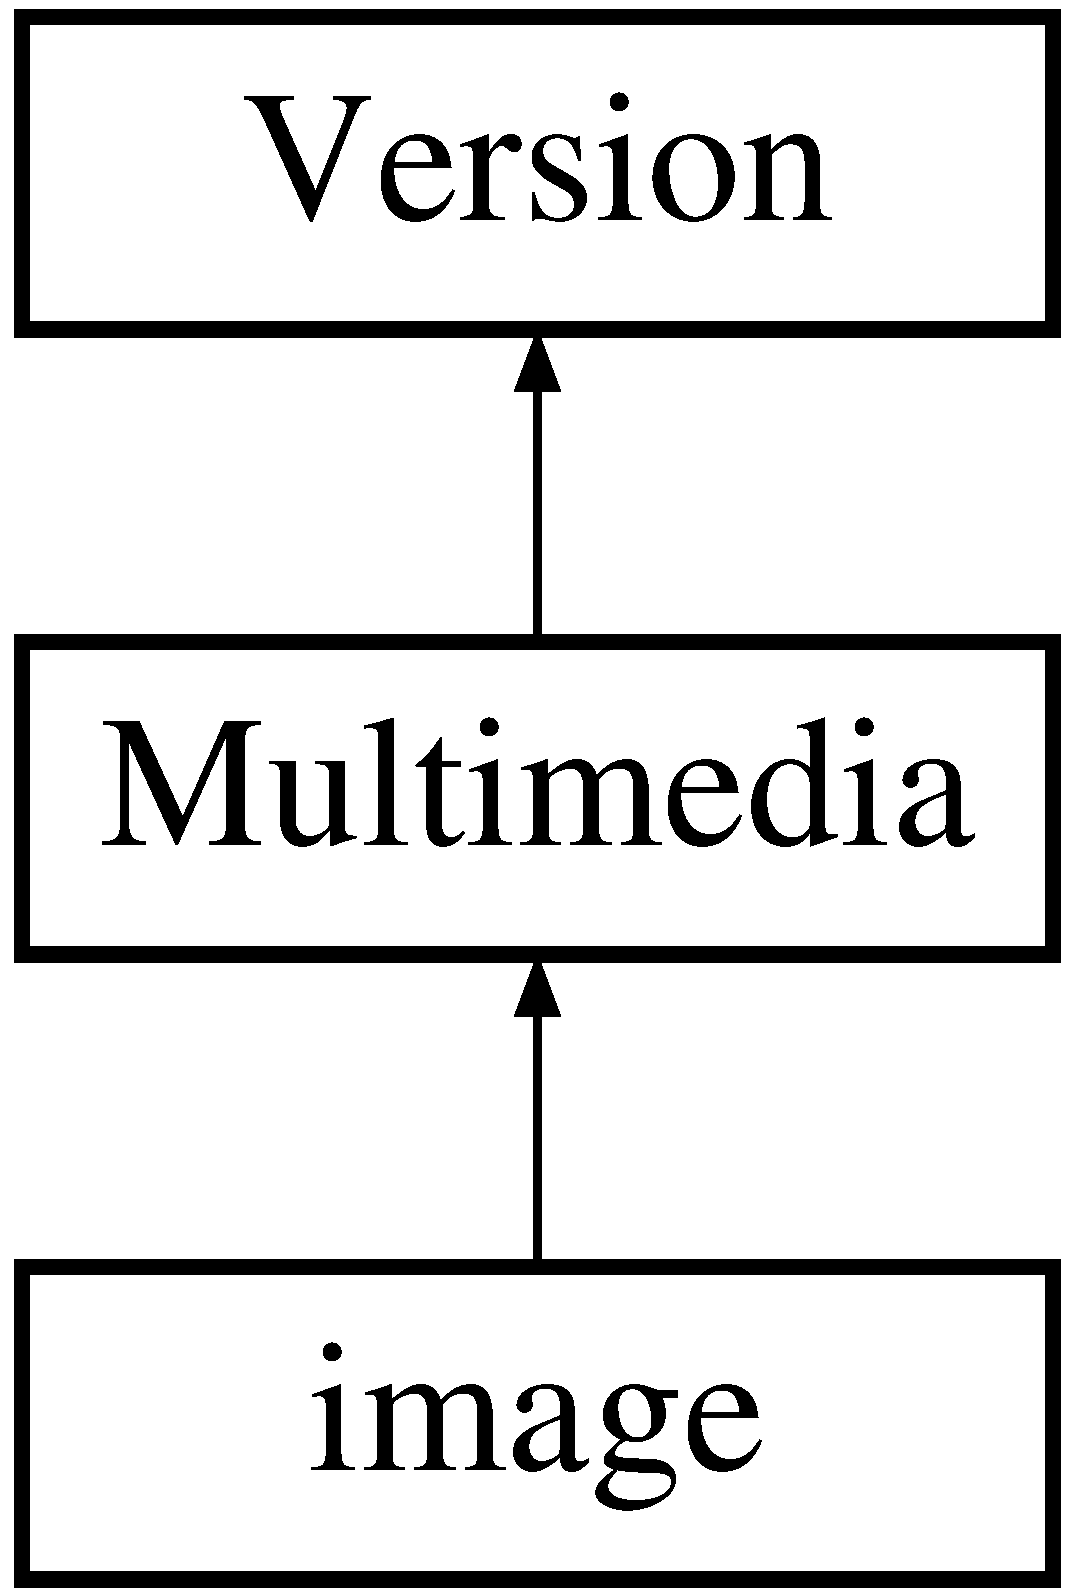
\includegraphics[height=3.000000cm]{classimage}
\end{center}
\end{figure}
\subsection*{Public Member Functions}
\begin{DoxyCompactItemize}
\item 
\mbox{\Hypertarget{classimage_abea77c75bedbc04610dbe4edcfc83b8e}\label{classimage_abea77c75bedbc04610dbe4edcfc83b8e}} 
{\bfseries image} (const Q\+String \&t, Q\+Date\+Time d, const Q\+String \&desc, const Q\+String \&i)
\item 
\mbox{\Hypertarget{classimage_a42db73028875ee5097f32b9e0983cf43}\label{classimage_a42db73028875ee5097f32b9e0983cf43}} 
const Q\+String \& {\bfseries get\+Img} () const
\item 
\mbox{\Hypertarget{classimage_a9c4f017fd62bf11a8cfdd56ea4f71f0f}\label{classimage_a9c4f017fd62bf11a8cfdd56ea4f71f0f}} 
void {\bfseries set\+Img} (const Q\+String \&img\+\_\+\+U\+RL)
\end{DoxyCompactItemize}


\subsection{Detailed Description}
Classe image hérite de \hyperlink{class_multimedia}{Multimedia}. 

\hyperlink{class_note}{Note} image {\itshape img} \+: Q\+String lien vers le fichier image. Ce lien est identique à celui de \hyperlink{class_multimedia}{Multimedia} 

The documentation for this class was generated from the following file\+:\begin{DoxyCompactItemize}
\item 
\hyperlink{multimedia_8h}{multimedia.\+h}\end{DoxyCompactItemize}

\hypertarget{class_interface}{}\section{Interface Class Reference}
\label{class_interface}\index{Interface@{Interface}}


The \hyperlink{class_interface}{Interface} class\+: heritate Q\+Main\+Window, this class is Main\+Window of the program.  




{\ttfamily \#include $<$winterface.\+h$>$}

Inheritance diagram for Interface\+:\begin{figure}[H]
\begin{center}
\leavevmode
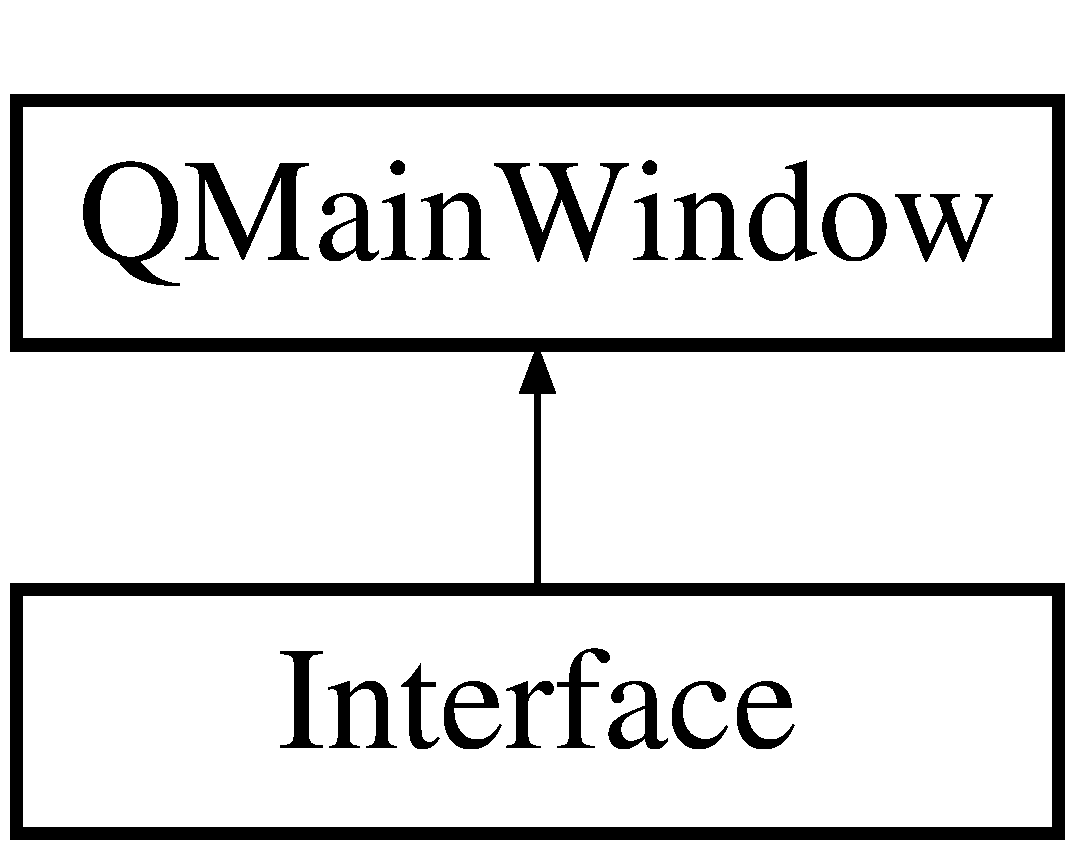
\includegraphics[height=2.000000cm]{class_interface}
\end{center}
\end{figure}
\subsection*{Public Slots}
\begin{DoxyCompactItemize}
\item 
\mbox{\Hypertarget{class_interface_a3a82b8958d8fa2dd8239f781c5c92042}\label{class_interface_a3a82b8958d8fa2dd8239f781c5c92042}} 
void \hyperlink{class_interface_a3a82b8958d8fa2dd8239f781c5c92042}{avant\+\_\+de\+\_\+fermer} ()
\begin{DoxyCompactList}\small\item\em avant\+\_\+de\+\_\+fermer\+: action perform before close totally program \end{DoxyCompactList}\item 
\mbox{\Hypertarget{class_interface_a94a88ff71e0b2caef92e88972662d4b0}\label{class_interface_a94a88ff71e0b2caef92e88972662d4b0}} 
void \hyperlink{class_interface_a94a88ff71e0b2caef92e88972662d4b0}{ouvrir\+\_\+relations} ()
\begin{DoxyCompactList}\small\item\em ouvrir\+\_\+relations\+: construct and show widget to view all the Relations \end{DoxyCompactList}\item 
\mbox{\Hypertarget{class_interface_ac5a8f808b693fc578f37b303aaf7ff1b}\label{class_interface_ac5a8f808b693fc578f37b303aaf7ff1b}} 
void \hyperlink{class_interface_ac5a8f808b693fc578f37b303aaf7ff1b}{ouvrir\+\_\+creer\+\_\+relation} ()
\begin{DoxyCompactList}\small\item\em ouvrir\+\_\+creer\+\_\+relation\+: construct and show widget to create \hyperlink{class_relation}{Relation} \end{DoxyCompactList}\item 
\mbox{\Hypertarget{class_interface_ab56822f065a7ef72d1db16964e0cbb4d}\label{class_interface_ab56822f065a7ef72d1db16964e0cbb4d}} 
void \hyperlink{class_interface_ab56822f065a7ef72d1db16964e0cbb4d}{ouvrir\+\_\+gauche} ()
\begin{DoxyCompactList}\small\item\em ouvrir\+\_\+gauche\+: construct and show widget to view all the notes (active and archived) \end{DoxyCompactList}\item 
\mbox{\Hypertarget{class_interface_a473b685de72a223d9972a70c0698e314}\label{class_interface_a473b685de72a223d9972a70c0698e314}} 
void \hyperlink{class_interface_a473b685de72a223d9972a70c0698e314}{ouvrir\+\_\+note\+\_\+active\+\_\+id} ()
\begin{DoxyCompactList}\small\item\em ouvrir\+\_\+note\+\_\+active\+\_\+id\+: construct and show widget to view note active with its versions \end{DoxyCompactList}\item 
\mbox{\Hypertarget{class_interface_a741673a4341956dba8eb4d6173931fca}\label{class_interface_a741673a4341956dba8eb4d6173931fca}} 
void \hyperlink{class_interface_a741673a4341956dba8eb4d6173931fca}{ouvrir\+\_\+note\+\_\+archivee\+\_\+id} ()
\begin{DoxyCompactList}\small\item\em ouvrir\+\_\+note\+\_\+archivee\+\_\+id\+: construct and show widget to view note archived with its versions \end{DoxyCompactList}\item 
\mbox{\Hypertarget{class_interface_a98b07127215c9316870987d49b2e0d3c}\label{class_interface_a98b07127215c9316870987d49b2e0d3c}} 
void \hyperlink{class_interface_a98b07127215c9316870987d49b2e0d3c}{ouvrir\+\_\+creer\+\_\+note} ()
\begin{DoxyCompactList}\small\item\em ouvrir\+\_\+creer\+\_\+note\+: construct and show widget to create a new note \end{DoxyCompactList}\item 
\mbox{\Hypertarget{class_interface_a2ebf4a5fd59fa36584671931daae622a}\label{class_interface_a2ebf4a5fd59fa36584671931daae622a}} 
void \hyperlink{class_interface_a2ebf4a5fd59fa36584671931daae622a}{forward\+\_\+to\+\_\+create\+\_\+type} ()
\begin{DoxyCompactList}\small\item\em forward\+\_\+to\+\_\+create\+\_\+type\+: construct and show widget form accordingly to the type of the note \end{DoxyCompactList}\item 
\mbox{\Hypertarget{class_interface_a326cdc1e75cc89190832376aaa56d3af}\label{class_interface_a326cdc1e75cc89190832376aaa56d3af}} 
void \hyperlink{class_interface_a326cdc1e75cc89190832376aaa56d3af}{restaurer\+\_\+note} ()
\begin{DoxyCompactList}\small\item\em restaurer\+\_\+note\+: restore the note which is archived \end{DoxyCompactList}\item 
\mbox{\Hypertarget{class_interface_ab4cdf89b7b6c8120c44625356a4987c1}\label{class_interface_ab4cdf89b7b6c8120c44625356a4987c1}} 
void \hyperlink{class_interface_ab4cdf89b7b6c8120c44625356a4987c1}{restaurer\+\_\+version} ()
\begin{DoxyCompactList}\small\item\em restaurer\+\_\+version\+: restore a version of a note active \end{DoxyCompactList}\item 
\mbox{\Hypertarget{class_interface_abb959eacc914a6618e9f4741b42706f7}\label{class_interface_abb959eacc914a6618e9f4741b42706f7}} 
void \hyperlink{class_interface_abb959eacc914a6618e9f4741b42706f7}{ouvrir\+\_\+version\+\_\+act} ()
\begin{DoxyCompactList}\small\item\em ouvrir\+\_\+version\+\_\+act\+: construct and show widget to view inside a version of a note active \end{DoxyCompactList}\item 
\mbox{\Hypertarget{class_interface_a81f01e8dec044f52338b2f650fa48bde}\label{class_interface_a81f01e8dec044f52338b2f650fa48bde}} 
void \hyperlink{class_interface_a81f01e8dec044f52338b2f650fa48bde}{ouvrir\+\_\+version\+\_\+arch} ()
\begin{DoxyCompactList}\small\item\em ouvrir\+\_\+version\+\_\+act\+: construct and show widget to view inside a version of a note archived \end{DoxyCompactList}\item 
\mbox{\Hypertarget{class_interface_a3a3d220b32fa6e4dda6f17f1899d1882}\label{class_interface_a3a3d220b32fa6e4dda6f17f1899d1882}} 
void \hyperlink{class_interface_a3a3d220b32fa6e4dda6f17f1899d1882}{sauver\+\_\+article} ()
\begin{DoxyCompactList}\small\item\em sauver\+\_\+article\+: save an \hyperlink{class_article}{Article} \end{DoxyCompactList}\item 
\mbox{\Hypertarget{class_interface_aaf757b3c67a42c5c42e0fd993ed2eb0e}\label{class_interface_aaf757b3c67a42c5c42e0fd993ed2eb0e}} 
void \hyperlink{class_interface_aaf757b3c67a42c5c42e0fd993ed2eb0e}{creer\+\_\+relation} ()
\begin{DoxyCompactList}\small\item\em creer\+\_\+relation\+: construct and show widget to create new relation \end{DoxyCompactList}\item 
\mbox{\Hypertarget{class_interface_addd6497067b6e680dee59e00726ea22e}\label{class_interface_addd6497067b6e680dee59e00726ea22e}} 
void \hyperlink{class_interface_addd6497067b6e680dee59e00726ea22e}{ouvrir\+\_\+couples} ()
\begin{DoxyCompactList}\small\item\em ouvrir\+\_\+couples\+: construct and show widget to view couples inside a relation \end{DoxyCompactList}\item 
\mbox{\Hypertarget{class_interface_a7f3dca1c4257a0af289a56dafe1c3025}\label{class_interface_a7f3dca1c4257a0af289a56dafe1c3025}} 
void \hyperlink{class_interface_a7f3dca1c4257a0af289a56dafe1c3025}{ouvrir\+\_\+creer\+\_\+couple} ()
\begin{DoxyCompactList}\small\item\em ouvrir\+\_\+creer\+\_\+couple\+: construct and show widget to create new couple \end{DoxyCompactList}\item 
\mbox{\Hypertarget{class_interface_a10c473d45e7063f2e556f3267b1df85f}\label{class_interface_a10c473d45e7063f2e556f3267b1df85f}} 
void \hyperlink{class_interface_a10c473d45e7063f2e556f3267b1df85f}{creer\+\_\+couple} ()
\begin{DoxyCompactList}\small\item\em ouvrir\+\_\+creer\+\_\+couple\+: construct and show widget to create new couple \end{DoxyCompactList}\end{DoxyCompactItemize}
\subsection*{Public Member Functions}
\begin{DoxyCompactItemize}
\item 
\mbox{\Hypertarget{class_interface_a4406d74c75bdfe150bf72be1f1cda8b1}\label{class_interface_a4406d74c75bdfe150bf72be1f1cda8b1}} 
\hyperlink{class_interface_a4406d74c75bdfe150bf72be1f1cda8b1}{Interface} ()
\begin{DoxyCompactList}\small\item\em \hyperlink{class_interface}{Interface}\+: initilize the \hyperlink{class_interface}{Interface}. \end{DoxyCompactList}\item 
\mbox{\Hypertarget{class_interface_a72f663f65f2f4f0f1c0cc710206c844f}\label{class_interface_a72f663f65f2f4f0f1c0cc710206c844f}} 
void \hyperlink{class_interface_a72f663f65f2f4f0f1c0cc710206c844f}{fermer\+\_\+droite} ()
\begin{DoxyCompactList}\small\item\em fermer\+\_\+droite\+: close whatever widgets which are opened on the right side of the \hyperlink{class_interface}{Interface} \end{DoxyCompactList}\item 
\mbox{\Hypertarget{class_interface_a82de37089406e4a81eae6b98d8c6f4e4}\label{class_interface_a82de37089406e4a81eae6b98d8c6f4e4}} 
void \hyperlink{class_interface_a82de37089406e4a81eae6b98d8c6f4e4}{fermer\+\_\+gauche} ()
\begin{DoxyCompactList}\small\item\em fermer\+\_\+gauche\+: close whatever widgets which are opened on the left side of the \hyperlink{class_interface}{Interface} \end{DoxyCompactList}\item 
\mbox{\Hypertarget{class_interface_a0089c8fe1279b59d283bf9bd50b43912}\label{class_interface_a0089c8fe1279b59d283bf9bd50b43912}} 
void \hyperlink{class_interface_a0089c8fe1279b59d283bf9bd50b43912}{fermer\+\_\+centre} ()
\begin{DoxyCompactList}\small\item\em fermer\+\_\+centre\+: close whatever widgets which are opened on the centre of the \hyperlink{class_interface}{Interface} \end{DoxyCompactList}\item 
void \hyperlink{class_interface_a5e55a321ae0f587fb2c1378aad7536cf}{close\+Event} (Q\+Close\+Event $\ast$bar)
\begin{DoxyCompactList}\small\item\em close\+Event\+: handle Event when click close button at the up-\/right corner of the \hyperlink{class_interface}{Interface} \end{DoxyCompactList}\end{DoxyCompactItemize}
\subsection*{Public Attributes}
\begin{DoxyCompactItemize}
\item 
\mbox{\Hypertarget{class_interface_a9ec3b9f9d2f43b773f04f22e49d439a8}\label{class_interface_a9ec3b9f9d2f43b773f04f22e49d439a8}} 
Q\+Action $\ast$ \hyperlink{class_interface_a9ec3b9f9d2f43b773f04f22e49d439a8}{action\+Corbeille\+Auto}
\begin{DoxyCompactList}\small\item\em action\+Corbeille\+Auto\+: this action bind to check to empty Corbeille when close program \end{DoxyCompactList}\end{DoxyCompactItemize}


\subsection{Detailed Description}
The \hyperlink{class_interface}{Interface} class\+: heritate Q\+Main\+Window, this class is Main\+Window of the program. 

All the widgets and events happen inside the \hyperlink{class_interface}{Interface} 

\subsection{Member Function Documentation}
\mbox{\Hypertarget{class_interface_a5e55a321ae0f587fb2c1378aad7536cf}\label{class_interface_a5e55a321ae0f587fb2c1378aad7536cf}} 
\index{Interface@{Interface}!close\+Event@{close\+Event}}
\index{close\+Event@{close\+Event}!Interface@{Interface}}
\subsubsection{\texorpdfstring{close\+Event()}{closeEvent()}}
{\footnotesize\ttfamily void Interface\+::close\+Event (\begin{DoxyParamCaption}\item[{Q\+Close\+Event $\ast$}]{bar }\end{DoxyParamCaption})}



close\+Event\+: handle Event when click close button at the up-\/right corner of the \hyperlink{class_interface}{Interface} 


\begin{DoxyParams}{Parameters}
{\em bar} & pointer to buttons \\
\hline
\end{DoxyParams}


The documentation for this class was generated from the following files\+:\begin{DoxyCompactItemize}
\item 
\hyperlink{winterface_8h}{winterface.\+h}\item 
winterface.\+cpp\end{DoxyCompactItemize}

\hypertarget{class_relation_1_1iterator}{}\section{Relation\+:\+:iterator Class Reference}
\label{class_relation_1_1iterator}\index{Relation\+::iterator@{Relation\+::iterator}}


The iterator class\+: iterator of relation, iterate throught the table of couple.  




{\ttfamily \#include $<$relation.\+h$>$}

Inheritance diagram for Relation\+:\+:iterator\+:\begin{figure}[H]
\begin{center}
\leavevmode
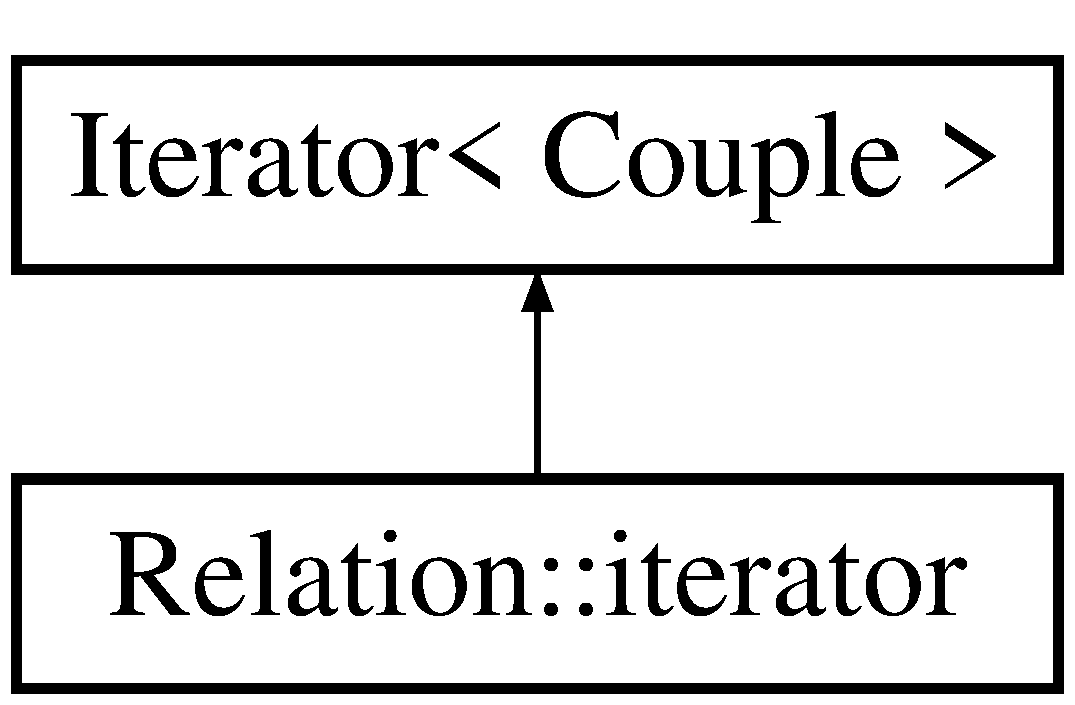
\includegraphics[height=2.000000cm]{class_relation_1_1iterator}
\end{center}
\end{figure}
\subsection*{Friends}
\begin{DoxyCompactItemize}
\item 
\mbox{\Hypertarget{class_relation_1_1iterator_a7ee004262f27f8c916688911a71e3aa1}\label{class_relation_1_1iterator_a7ee004262f27f8c916688911a71e3aa1}} 
class {\bfseries Relation}
\end{DoxyCompactItemize}
\subsection*{Additional Inherited Members}


\subsection{Detailed Description}
The iterator class\+: iterator of relation, iterate throught the table of couple. 

The documentation for this class was generated from the following file\+:\begin{DoxyCompactItemize}
\item 
\hyperlink{relation_8h}{relation.\+h}\end{DoxyCompactItemize}

\hypertarget{class_iterator}{}\section{Iterator$<$ T $>$ Class Template Reference}
\label{class_iterator}\index{Iterator$<$ T $>$@{Iterator$<$ T $>$}}
\subsection*{Public Member Functions}
\begin{DoxyCompactItemize}
\item 
\mbox{\Hypertarget{class_iterator_a87d4af70ba6312e91e1ab6a7c9e2ec6d}\label{class_iterator_a87d4af70ba6312e91e1ab6a7c9e2ec6d}} 
\hyperlink{class_iterator_a87d4af70ba6312e91e1ab6a7c9e2ec6d}{Iterator} ()
\begin{DoxyCompactList}\small\item\em \hyperlink{class_iterator}{Iterator}\+: constructor by default. \end{DoxyCompactList}\item 
T $\ast$ \hyperlink{class_iterator_a10ab6542ca4a31393939291780fa7fa2}{operator$\ast$} () const
\begin{DoxyCompactList}\small\item\em operator $\ast$\+: get the pointer of current element \end{DoxyCompactList}\item 
\hyperlink{class_iterator}{Iterator} \& \hyperlink{class_iterator_a7f820677fc6ee38192e0457090646cd6}{operator++} ()
\begin{DoxyCompactList}\small\item\em operator ++\+: pre-\/increment iterator \end{DoxyCompactList}\item 
\hyperlink{class_iterator}{Iterator} \& \hyperlink{class_iterator_a292066a3edaea39abf09e6a14328c489}{operator++} (int)
\begin{DoxyCompactList}\small\item\em \hyperlink{class_iterator_a292066a3edaea39abf09e6a14328c489}{operator ++(int)}\+: post-\/increment iterator \end{DoxyCompactList}\item 
\hyperlink{class_iterator}{Iterator} \& \hyperlink{class_iterator_a580d645f1163cd20b92b469477324509}{operator-\/-\/} ()
\begin{DoxyCompactList}\small\item\em operator --\+: pre-\/decrement iterator \end{DoxyCompactList}\item 
\hyperlink{class_iterator}{Iterator} \& \hyperlink{class_iterator_a96b7f620a07d11a31335e8b43609625e}{operator-\/-\/} (int)
\begin{DoxyCompactList}\small\item\em operator --\+: post-\/decrement iterator \end{DoxyCompactList}\item 
bool \hyperlink{class_iterator_a81ed85772dc6f8251fc5d65cf57b7fa8}{operator==} (\hyperlink{class_iterator}{Iterator} it) const
\begin{DoxyCompactList}\small\item\em operator ==\+: comparaison of iterator \end{DoxyCompactList}\item 
bool \hyperlink{class_iterator_a5e8725bfbba9901f8148e427a9b8886a}{operator!=} (\hyperlink{class_iterator}{Iterator} it) const
\begin{DoxyCompactList}\small\item\em operator !=\+: comparaison of iterator \end{DoxyCompactList}\end{DoxyCompactItemize}
\subsection*{Protected Member Functions}
\begin{DoxyCompactItemize}
\item 
\hyperlink{class_iterator_a8d10287aafe1cac58db300c53c2a3f8c}{Iterator} (T $\ast$$\ast$curr)
\begin{DoxyCompactList}\small\item\em \hyperlink{class_iterator}{Iterator}\+: constructor of iterator. \end{DoxyCompactList}\end{DoxyCompactItemize}


\subsection{Constructor \& Destructor Documentation}
\mbox{\Hypertarget{class_iterator_a8d10287aafe1cac58db300c53c2a3f8c}\label{class_iterator_a8d10287aafe1cac58db300c53c2a3f8c}} 
\index{Iterator@{Iterator}!Iterator@{Iterator}}
\index{Iterator@{Iterator}!Iterator@{Iterator}}
\subsubsection{\texorpdfstring{Iterator()}{Iterator()}}
{\footnotesize\ttfamily template$<$class T$>$ \\
\hyperlink{class_iterator}{Iterator}$<$ T $>$\+::\hyperlink{class_iterator}{Iterator} (\begin{DoxyParamCaption}\item[{T $\ast$$\ast$}]{curr }\end{DoxyParamCaption})\hspace{0.3cm}{\ttfamily [inline]}, {\ttfamily [protected]}}



\hyperlink{class_iterator}{Iterator}\+: constructor of iterator. 


\begin{DoxyParams}{Parameters}
{\em curr} & pointer to an position of the table of T \\
\hline
\end{DoxyParams}


\subsection{Member Function Documentation}
\mbox{\Hypertarget{class_iterator_a5e8725bfbba9901f8148e427a9b8886a}\label{class_iterator_a5e8725bfbba9901f8148e427a9b8886a}} 
\index{Iterator@{Iterator}!operator"!=@{operator"!=}}
\index{operator"!=@{operator"!=}!Iterator@{Iterator}}
\subsubsection{\texorpdfstring{operator"!=()}{operator!=()}}
{\footnotesize\ttfamily template$<$class T$>$ \\
bool \hyperlink{class_iterator}{Iterator}$<$ T $>$\+::operator!= (\begin{DoxyParamCaption}\item[{\hyperlink{class_iterator}{Iterator}$<$ T $>$}]{it }\end{DoxyParamCaption}) const\hspace{0.3cm}{\ttfamily [inline]}}



operator !=\+: comparaison of iterator 

\begin{DoxyReturn}{Returns}
true if not same position 
\end{DoxyReturn}
\mbox{\Hypertarget{class_iterator_a10ab6542ca4a31393939291780fa7fa2}\label{class_iterator_a10ab6542ca4a31393939291780fa7fa2}} 
\index{Iterator@{Iterator}!operator$\ast$@{operator$\ast$}}
\index{operator$\ast$@{operator$\ast$}!Iterator@{Iterator}}
\subsubsection{\texorpdfstring{operator$\ast$()}{operator*()}}
{\footnotesize\ttfamily template$<$class T$>$ \\
T$\ast$ \hyperlink{class_iterator}{Iterator}$<$ T $>$\+::operator$\ast$ (\begin{DoxyParamCaption}{ }\end{DoxyParamCaption}) const\hspace{0.3cm}{\ttfamily [inline]}}



operator $\ast$\+: get the pointer of current element 

\begin{DoxyReturn}{Returns}
pointer of type T 
\end{DoxyReturn}
\mbox{\Hypertarget{class_iterator_a7f820677fc6ee38192e0457090646cd6}\label{class_iterator_a7f820677fc6ee38192e0457090646cd6}} 
\index{Iterator@{Iterator}!operator++@{operator++}}
\index{operator++@{operator++}!Iterator@{Iterator}}
\subsubsection{\texorpdfstring{operator++()}{operator++()}\hspace{0.1cm}{\footnotesize\ttfamily [1/2]}}
{\footnotesize\ttfamily template$<$class T$>$ \\
\hyperlink{class_iterator}{Iterator}\& \hyperlink{class_iterator}{Iterator}$<$ T $>$\+::operator++ (\begin{DoxyParamCaption}{ }\end{DoxyParamCaption})\hspace{0.3cm}{\ttfamily [inline]}}



operator ++\+: pre-\/increment iterator 

\begin{DoxyReturn}{Returns}
iterator\& 
\end{DoxyReturn}
\mbox{\Hypertarget{class_iterator_a292066a3edaea39abf09e6a14328c489}\label{class_iterator_a292066a3edaea39abf09e6a14328c489}} 
\index{Iterator@{Iterator}!operator++@{operator++}}
\index{operator++@{operator++}!Iterator@{Iterator}}
\subsubsection{\texorpdfstring{operator++()}{operator++()}\hspace{0.1cm}{\footnotesize\ttfamily [2/2]}}
{\footnotesize\ttfamily template$<$class T$>$ \\
\hyperlink{class_iterator}{Iterator}\& \hyperlink{class_iterator}{Iterator}$<$ T $>$\+::operator++ (\begin{DoxyParamCaption}\item[{int}]{ }\end{DoxyParamCaption})\hspace{0.3cm}{\ttfamily [inline]}}



\hyperlink{class_iterator_a292066a3edaea39abf09e6a14328c489}{operator ++(int)}\+: post-\/increment iterator 

\begin{DoxyReturn}{Returns}
iterator\& 
\end{DoxyReturn}
\mbox{\Hypertarget{class_iterator_a580d645f1163cd20b92b469477324509}\label{class_iterator_a580d645f1163cd20b92b469477324509}} 
\index{Iterator@{Iterator}!operator-\/-\/@{operator-\/-\/}}
\index{operator-\/-\/@{operator-\/-\/}!Iterator@{Iterator}}
\subsubsection{\texorpdfstring{operator-\/-\/()}{operator--()}\hspace{0.1cm}{\footnotesize\ttfamily [1/2]}}
{\footnotesize\ttfamily template$<$class T$>$ \\
\hyperlink{class_iterator}{Iterator}\& \hyperlink{class_iterator}{Iterator}$<$ T $>$\+::operator-\/-\/ (\begin{DoxyParamCaption}{ }\end{DoxyParamCaption})\hspace{0.3cm}{\ttfamily [inline]}}



operator --\+: pre-\/decrement iterator 

\begin{DoxyReturn}{Returns}
iterator\& 
\end{DoxyReturn}
\mbox{\Hypertarget{class_iterator_a96b7f620a07d11a31335e8b43609625e}\label{class_iterator_a96b7f620a07d11a31335e8b43609625e}} 
\index{Iterator@{Iterator}!operator-\/-\/@{operator-\/-\/}}
\index{operator-\/-\/@{operator-\/-\/}!Iterator@{Iterator}}
\subsubsection{\texorpdfstring{operator-\/-\/()}{operator--()}\hspace{0.1cm}{\footnotesize\ttfamily [2/2]}}
{\footnotesize\ttfamily template$<$class T$>$ \\
\hyperlink{class_iterator}{Iterator}\& \hyperlink{class_iterator}{Iterator}$<$ T $>$\+::operator-\/-\/ (\begin{DoxyParamCaption}\item[{int}]{ }\end{DoxyParamCaption})\hspace{0.3cm}{\ttfamily [inline]}}



operator --\+: post-\/decrement iterator 

\begin{DoxyReturn}{Returns}
iterator\& 
\end{DoxyReturn}
\mbox{\Hypertarget{class_iterator_a81ed85772dc6f8251fc5d65cf57b7fa8}\label{class_iterator_a81ed85772dc6f8251fc5d65cf57b7fa8}} 
\index{Iterator@{Iterator}!operator==@{operator==}}
\index{operator==@{operator==}!Iterator@{Iterator}}
\subsubsection{\texorpdfstring{operator==()}{operator==()}}
{\footnotesize\ttfamily template$<$class T$>$ \\
bool \hyperlink{class_iterator}{Iterator}$<$ T $>$\+::operator== (\begin{DoxyParamCaption}\item[{\hyperlink{class_iterator}{Iterator}$<$ T $>$}]{it }\end{DoxyParamCaption}) const\hspace{0.3cm}{\ttfamily [inline]}}



operator ==\+: comparaison of iterator 

\begin{DoxyReturn}{Returns}
true if same position 
\end{DoxyReturn}


The documentation for this class was generated from the following file\+:\begin{DoxyCompactItemize}
\item 
\hyperlink{iterator_8h}{iterator.\+h}\end{DoxyCompactItemize}

\hypertarget{class_relation_manager_1_1iterator}{}\section{Relation\+Manager\+:\+:iterator Class Reference}
\label{class_relation_manager_1_1iterator}\index{Relation\+Manager\+::iterator@{Relation\+Manager\+::iterator}}


The iterator class\+: iterator through table of relations.  




{\ttfamily \#include $<$relation.\+h$>$}

Inheritance diagram for Relation\+Manager\+:\+:iterator\+:\begin{figure}[H]
\begin{center}
\leavevmode
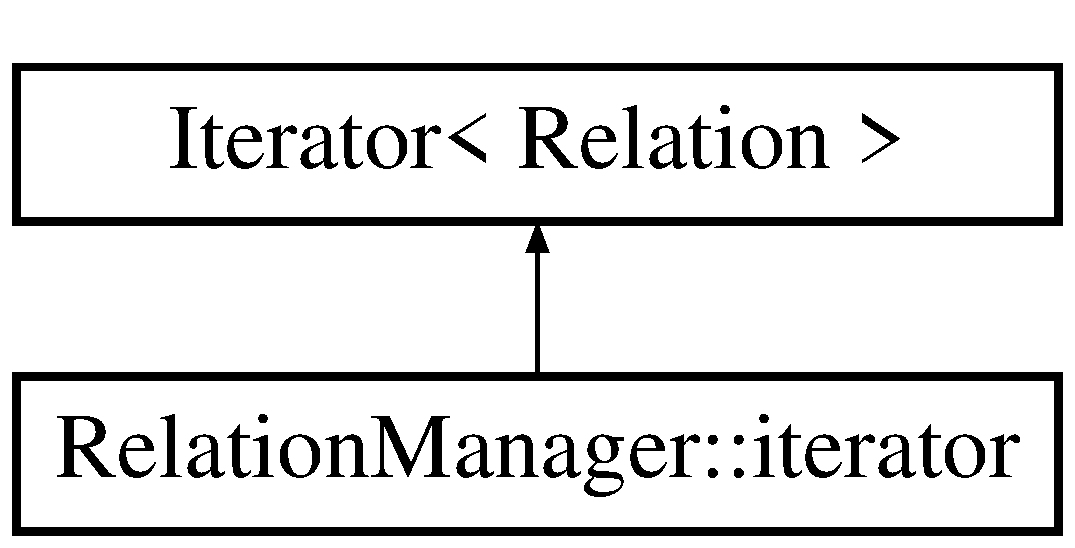
\includegraphics[height=2.000000cm]{class_relation_manager_1_1iterator}
\end{center}
\end{figure}
\subsection*{Friends}
\begin{DoxyCompactItemize}
\item 
\mbox{\Hypertarget{class_relation_manager_1_1iterator_a55fae9c2e48742dd0a8596e6d8721775}\label{class_relation_manager_1_1iterator_a55fae9c2e48742dd0a8596e6d8721775}} 
class {\bfseries Relation\+Manager}
\end{DoxyCompactItemize}
\subsection*{Additional Inherited Members}


\subsection{Detailed Description}
The iterator class\+: iterator through table of relations. 

The documentation for this class was generated from the following file\+:\begin{DoxyCompactItemize}
\item 
\hyperlink{relation_8h}{relation.\+h}\end{DoxyCompactItemize}

\hypertarget{class_note_1_1iterator}{}\section{Note\+:\+:iterator Class Reference}
\label{class_note_1_1iterator}\index{Note\+::iterator@{Note\+::iterator}}
Inheritance diagram for Note\+:\+:iterator\+:\begin{figure}[H]
\begin{center}
\leavevmode
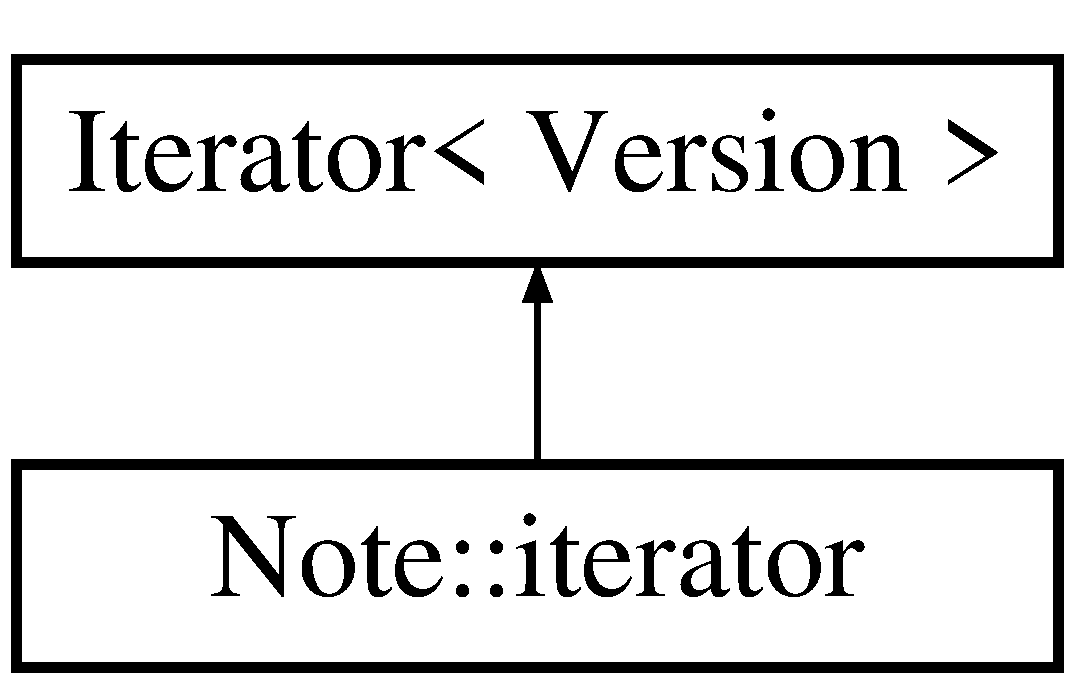
\includegraphics[height=2.000000cm]{class_note_1_1iterator}
\end{center}
\end{figure}
\subsection*{Friends}
\begin{DoxyCompactItemize}
\item 
\mbox{\Hypertarget{class_note_1_1iterator_a93d7e72623acdfa5b079a11fbf2d9f9d}\label{class_note_1_1iterator_a93d7e72623acdfa5b079a11fbf2d9f9d}} 
class {\bfseries Note}
\end{DoxyCompactItemize}
\subsection*{Additional Inherited Members}


The documentation for this class was generated from the following file\+:\begin{DoxyCompactItemize}
\item 
\hyperlink{note_8h}{note.\+h}\end{DoxyCompactItemize}

\hypertarget{class_notes_manager_1_1iterator}{}\section{Notes\+Manager\+:\+:iterator Class Reference}
\label{class_notes_manager_1_1iterator}\index{Notes\+Manager\+::iterator@{Notes\+Manager\+::iterator}}
Inheritance diagram for Notes\+Manager\+:\+:iterator\+:\begin{figure}[H]
\begin{center}
\leavevmode
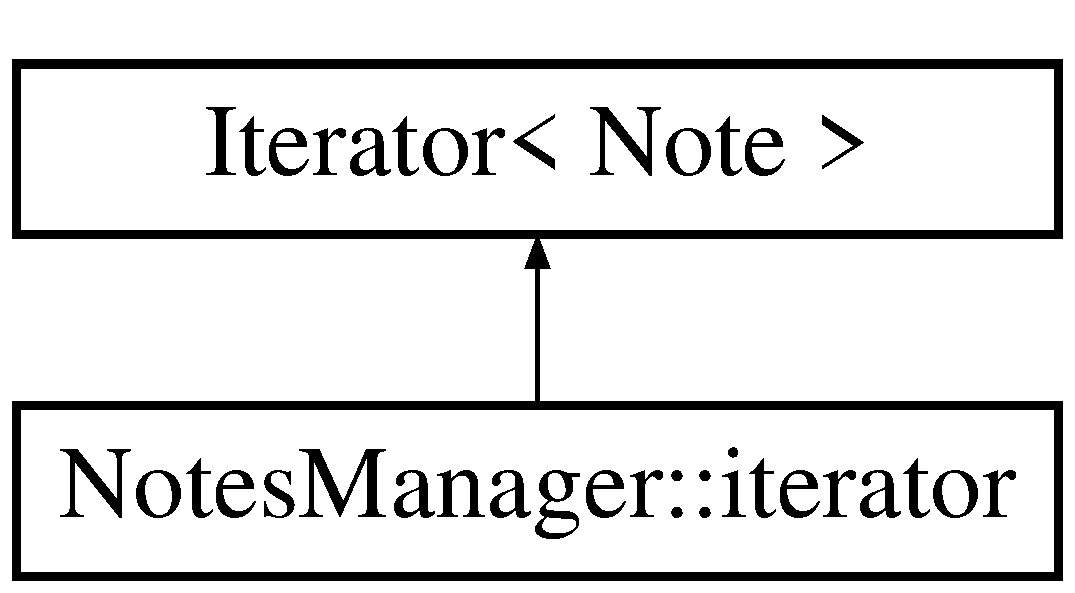
\includegraphics[height=2.000000cm]{class_notes_manager_1_1iterator}
\end{center}
\end{figure}
\subsection*{Friends}
\begin{DoxyCompactItemize}
\item 
\mbox{\Hypertarget{class_notes_manager_1_1iterator_a017a5144e8cfa6087305055ab968ef41}\label{class_notes_manager_1_1iterator_a017a5144e8cfa6087305055ab968ef41}} 
class {\bfseries Notes\+Manager}
\end{DoxyCompactItemize}
\subsection*{Additional Inherited Members}


The documentation for this class was generated from the following file\+:\begin{DoxyCompactItemize}
\item 
\hyperlink{notesmanager_8h}{notesmanager.\+h}\end{DoxyCompactItemize}

\hypertarget{class_multimedia}{}\section{Multimedia Class Reference}
\label{class_multimedia}\index{Multimedia@{Multimedia}}


Définit la classe \hyperlink{class_multimedia}{Multimedia} et ses classes filles (image, audio, video)  




{\ttfamily \#include $<$multimedia.\+h$>$}

Inheritance diagram for Multimedia\+:\begin{figure}[H]
\begin{center}
\leavevmode
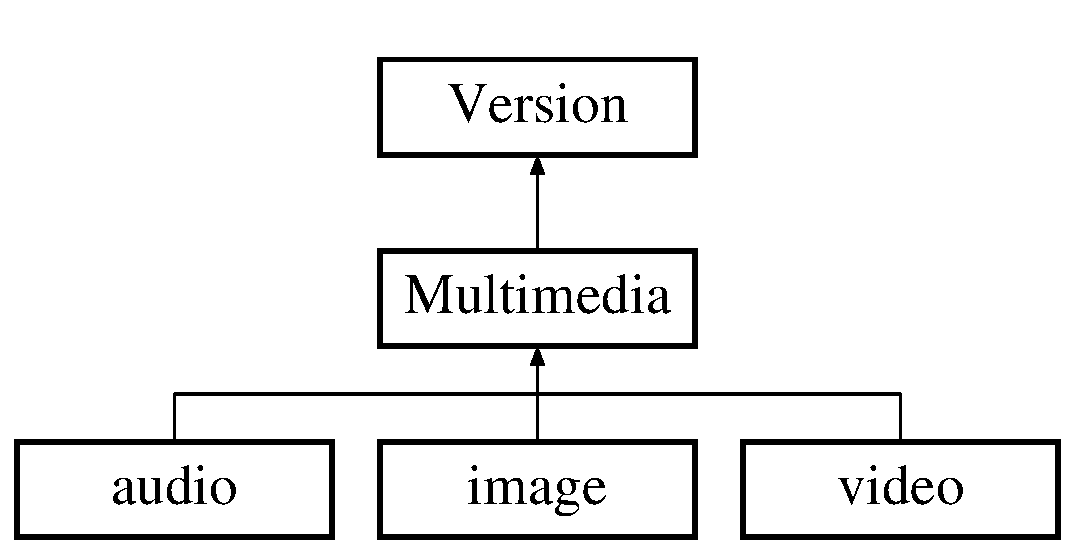
\includegraphics[height=3.000000cm]{class_multimedia}
\end{center}
\end{figure}
\subsection*{Public Member Functions}
\begin{DoxyCompactItemize}
\item 
\mbox{\Hypertarget{class_multimedia_ae51e2ff4de8074f01ddd7806d3ee123b}\label{class_multimedia_ae51e2ff4de8074f01ddd7806d3ee123b}} 
{\bfseries Multimedia} (const Q\+String \&t, Q\+Date\+Time d, const Q\+String \&desc, const Q\+String \&i)
\item 
\mbox{\Hypertarget{class_multimedia_a5036bb76fb0e9e0fc30fab727c2153bf}\label{class_multimedia_a5036bb76fb0e9e0fc30fab727c2153bf}} 
const Q\+String \& {\bfseries get\+Desc} () const
\item 
\mbox{\Hypertarget{class_multimedia_a8b55367c43e2ce9d450f9592201d3ffe}\label{class_multimedia_a8b55367c43e2ce9d450f9592201d3ffe}} 
const Q\+String \& {\bfseries getimg\+\_\+\+U\+RL} () const
\item 
\mbox{\Hypertarget{class_multimedia_adf3ef3a343c056e8c07b8715a0997735}\label{class_multimedia_adf3ef3a343c056e8c07b8715a0997735}} 
void {\bfseries set\+Desc} (const Q\+String \&new\+Desc)
\item 
\mbox{\Hypertarget{class_multimedia_a8f259550cd3078df95fcd8323d598632}\label{class_multimedia_a8f259550cd3078df95fcd8323d598632}} 
void {\bfseries set\+Img\+\_\+\+U\+RL} (const Q\+String \&new\+Img\+\_\+\+U\+RL)
\item 
void \hyperlink{class_multimedia_ac9c5f340806cbf1b93e8268c5c28ff92}{show\+Img} () const
\end{DoxyCompactItemize}


\subsection{Detailed Description}
Définit la classe \hyperlink{class_multimedia}{Multimedia} et ses classes filles (image, audio, video) 

Classe abstraite {\itshape desc\+:} Description {\itshape img\+\_\+\+U\+RL} \+: Fichier image 

\subsection{Member Function Documentation}
\mbox{\Hypertarget{class_multimedia_ac9c5f340806cbf1b93e8268c5c28ff92}\label{class_multimedia_ac9c5f340806cbf1b93e8268c5c28ff92}} 
\index{Multimedia@{Multimedia}!show\+Img@{show\+Img}}
\index{show\+Img@{show\+Img}!Multimedia@{Multimedia}}
\subsubsection{\texorpdfstring{show\+Img()}{showImg()}}
{\footnotesize\ttfamily void Multimedia\+::show\+Img (\begin{DoxyParamCaption}{ }\end{DoxyParamCaption}) const}

Affiche le fichier image 

The documentation for this class was generated from the following files\+:\begin{DoxyCompactItemize}
\item 
\hyperlink{multimedia_8h}{multimedia.\+h}\item 
multimedia.\+cpp\end{DoxyCompactItemize}

\hypertarget{class_note}{}\section{Note Class Reference}
\label{class_note}\index{Note@{Note}}


Définit la classe Notes \+: Permet de d\textquotesingle{}ajouter, supprimer, restaurer une \hyperlink{class_version}{Version} à une \hyperlink{class_note}{Note}.  




{\ttfamily \#include $<$note.\+h$>$}

\subsection*{Classes}
\begin{DoxyCompactItemize}
\item 
class \hyperlink{class_note_1_1iterator}{iterator}
\end{DoxyCompactItemize}
\subsection*{Public Member Functions}
\begin{DoxyCompactItemize}
\item 
\mbox{\Hypertarget{class_note_a74953ca0f81bb48c57bfc398bd0dc86a}\label{class_note_a74953ca0f81bb48c57bfc398bd0dc86a}} 
{\bfseries Note} (const Q\+String \&id, unsigned int nbmax=10, const \hyperlink{note_8h_a952f39258bbc825f3d94ffd41440486b}{Type\+\_\+etat\+\_\+note} \&e=active)
\item 
\mbox{\Hypertarget{class_note_aff851c4b14e763f5e00755a3a12fbe76}\label{class_note_aff851c4b14e763f5e00755a3a12fbe76}} 
const Q\+String \& {\bfseries get\+Id} () const
\item 
\mbox{\Hypertarget{class_note_ab5007eef00e371eada1b31ce2afe15d3}\label{class_note_ab5007eef00e371eada1b31ce2afe15d3}} 
unsigned int {\bfseries get\+Nb\+Version} () const
\item 
\mbox{\Hypertarget{class_note_ae967accab8c1783536e3dd49bfe87098}\label{class_note_ae967accab8c1783536e3dd49bfe87098}} 
unsigned int {\bfseries get\+Nb\+Max\+Version} () const
\item 
\mbox{\Hypertarget{class_note_a2db69efc8a682af2b404a05df78edd63}\label{class_note_a2db69efc8a682af2b404a05df78edd63}} 
const Q\+Date\+Time \& {\bfseries get\+Date\+Creation} () const
\item 
\mbox{\Hypertarget{class_note_a36ef7b5d9687d36aba0baf626a125d86}\label{class_note_a36ef7b5d9687d36aba0baf626a125d86}} 
const \hyperlink{note_8h_a952f39258bbc825f3d94ffd41440486b}{Type\+\_\+etat\+\_\+note} \& {\bfseries get\+Etat} () const
\item 
\mbox{\Hypertarget{class_note_aa53e04aa5c6c39867eb10b5b5f274f93}\label{class_note_aa53e04aa5c6c39867eb10b5b5f274f93}} 
void {\bfseries set\+Etat} (const \hyperlink{note_8h_a952f39258bbc825f3d94ffd41440486b}{Type\+\_\+etat\+\_\+note} e)
\item 
\mbox{\Hypertarget{class_note_a015599af2e64410923961d9ef6b3e18d}\label{class_note_a015599af2e64410923961d9ef6b3e18d}} 
\hyperlink{class_version}{Version} $\ast$ {\bfseries get\+Version} (const unsigned int p)
\item 
\mbox{\Hypertarget{class_note_a300a142b7cb07872522b6d16b4c77524}\label{class_note_a300a142b7cb07872522b6d16b4c77524}} 
\hyperlink{class_version}{Version} $\ast$ {\bfseries get\+Last\+Version} () const
\item 
void \hyperlink{class_note_a6a150fba840245d5c99c058e3457e775}{ajouter\+Version} (\hyperlink{class_version}{Version} $\ast$v)
\begin{DoxyCompactList}\small\item\em \+: Ajoute une version à une note \end{DoxyCompactList}\item 
void \hyperlink{class_note_a19cfb61168f8f6ce29cbdefd8448c0c0}{restaurer\+Version} (const unsigned int p)
\begin{DoxyCompactList}\small\item\em Restaurer une version d\textquotesingle{}une note. \end{DoxyCompactList}\item 
bool \hyperlink{class_note_aca74abbfeb1ff6bba66db5e81f5f622e}{is\+\_\+active} ()
\begin{DoxyCompactList}\small\item\em Cherche si la \hyperlink{class_note}{Note} est active. \end{DoxyCompactList}\item 
bool \hyperlink{class_note_a59f2e98d827736fefc03a71606db7e3d}{is\+\_\+archived} ()
\begin{DoxyCompactList}\small\item\em Cherche si la \hyperlink{class_note}{Note} est archivée. \end{DoxyCompactList}\item 
bool \hyperlink{class_note_a35ed46ae39aedc142d4fd9461a3d6a33}{is\+\_\+reprieved} ()
\begin{DoxyCompactList}\small\item\em Cherche si la \hyperlink{class_note}{Note} est en sursis. \end{DoxyCompactList}\item 
\mbox{\Hypertarget{class_note_a6104d75b44e1c93b2b30b5359746b1db}\label{class_note_a6104d75b44e1c93b2b30b5359746b1db}} 
\hyperlink{class_note_1_1iterator}{iterator} {\bfseries begin} ()
\item 
\mbox{\Hypertarget{class_note_a124c8d9a817ba9531c02750b7e56ad4c}\label{class_note_a124c8d9a817ba9531c02750b7e56ad4c}} 
\hyperlink{class_note_1_1iterator}{iterator} {\bfseries end} ()
\end{DoxyCompactItemize}


\subsection{Detailed Description}
Définit la classe Notes \+: Permet de d\textquotesingle{}ajouter, supprimer, restaurer une \hyperlink{class_version}{Version} à une \hyperlink{class_note}{Note}. 

Design Pattern \+: \hyperlink{class_iterator}{Iterator}. {\itshape id} \+: identifiant de la note \+: {\bfseries unique} {\itshape version} \+: tableau de pointeur de \hyperlink{class_version}{Version} {\itshape nb\+Version} \+: nombre de versions de la note {\itshape nb\+Max\+Version} \+: nombre de versions maximales de la note {\itshape etat} \+: Etat de la note {\itshape date\+\_\+creation} \+: Date de création de la note 

\subsection{Member Function Documentation}
\mbox{\Hypertarget{class_note_a6a150fba840245d5c99c058e3457e775}\label{class_note_a6a150fba840245d5c99c058e3457e775}} 
\index{Note@{Note}!ajouter\+Version@{ajouter\+Version}}
\index{ajouter\+Version@{ajouter\+Version}!Note@{Note}}
\subsubsection{\texorpdfstring{ajouter\+Version()}{ajouterVersion()}}
{\footnotesize\ttfamily void Note\+::ajouter\+Version (\begin{DoxyParamCaption}\item[{\hyperlink{class_version}{Version} $\ast$}]{v }\end{DoxyParamCaption})}



\+: Ajoute une version à une note 


\begin{DoxyParams}{Parameters}
{\em v} & \+: \hyperlink{class_version}{Version} d\textquotesingle{}une note \\
\hline
\end{DoxyParams}
\mbox{\Hypertarget{class_note_aca74abbfeb1ff6bba66db5e81f5f622e}\label{class_note_aca74abbfeb1ff6bba66db5e81f5f622e}} 
\index{Note@{Note}!is\+\_\+active@{is\+\_\+active}}
\index{is\+\_\+active@{is\+\_\+active}!Note@{Note}}
\subsubsection{\texorpdfstring{is\+\_\+active()}{is\_active()}}
{\footnotesize\ttfamily bool Note\+::is\+\_\+active (\begin{DoxyParamCaption}{ }\end{DoxyParamCaption})\hspace{0.3cm}{\ttfamily [inline]}}



Cherche si la \hyperlink{class_note}{Note} est active. 

\begin{DoxyReturn}{Returns}
1 si \hyperlink{class_note}{Note} est active, 0 sinon 
\end{DoxyReturn}
\mbox{\Hypertarget{class_note_a59f2e98d827736fefc03a71606db7e3d}\label{class_note_a59f2e98d827736fefc03a71606db7e3d}} 
\index{Note@{Note}!is\+\_\+archived@{is\+\_\+archived}}
\index{is\+\_\+archived@{is\+\_\+archived}!Note@{Note}}
\subsubsection{\texorpdfstring{is\+\_\+archived()}{is\_archived()}}
{\footnotesize\ttfamily bool Note\+::is\+\_\+archived (\begin{DoxyParamCaption}{ }\end{DoxyParamCaption})\hspace{0.3cm}{\ttfamily [inline]}}



Cherche si la \hyperlink{class_note}{Note} est archivée. 

\begin{DoxyReturn}{Returns}
1 si \hyperlink{class_note}{Note} est archivée, 0 sinon 
\end{DoxyReturn}
\mbox{\Hypertarget{class_note_a35ed46ae39aedc142d4fd9461a3d6a33}\label{class_note_a35ed46ae39aedc142d4fd9461a3d6a33}} 
\index{Note@{Note}!is\+\_\+reprieved@{is\+\_\+reprieved}}
\index{is\+\_\+reprieved@{is\+\_\+reprieved}!Note@{Note}}
\subsubsection{\texorpdfstring{is\+\_\+reprieved()}{is\_reprieved()}}
{\footnotesize\ttfamily bool Note\+::is\+\_\+reprieved (\begin{DoxyParamCaption}{ }\end{DoxyParamCaption})\hspace{0.3cm}{\ttfamily [inline]}}



Cherche si la \hyperlink{class_note}{Note} est en sursis. 

\begin{DoxyReturn}{Returns}
1 si \hyperlink{class_note}{Note} est en sursis, 0 sinon 
\end{DoxyReturn}
\mbox{\Hypertarget{class_note_a19cfb61168f8f6ce29cbdefd8448c0c0}\label{class_note_a19cfb61168f8f6ce29cbdefd8448c0c0}} 
\index{Note@{Note}!restaurer\+Version@{restaurer\+Version}}
\index{restaurer\+Version@{restaurer\+Version}!Note@{Note}}
\subsubsection{\texorpdfstring{restaurer\+Version()}{restaurerVersion()}}
{\footnotesize\ttfamily void Note\+::restaurer\+Version (\begin{DoxyParamCaption}\item[{const unsigned int}]{p }\end{DoxyParamCaption})}



Restaurer une version d\textquotesingle{}une note. 


\begin{DoxyParams}{Parameters}
{\em p} & \\
\hline
\end{DoxyParams}


The documentation for this class was generated from the following files\+:\begin{DoxyCompactItemize}
\item 
\hyperlink{note_8h}{note.\+h}\item 
note.\+cpp\end{DoxyCompactItemize}

\hypertarget{class_notes_manager}{}\section{Notes\+Manager Class Reference}
\label{class_notes_manager}\index{Notes\+Manager@{Notes\+Manager}}


Définit la classe \hyperlink{class_notes_manager}{Notes\+Manager} \+: Permet de d\textquotesingle{}ajouter, supprimer, restaurer une \hyperlink{class_note}{Note}. Permet de sauvegarder/charger la session dans/à partir d\textquotesingle{}un fichier X\+ML.  




{\ttfamily \#include $<$notesmanager.\+h$>$}

\subsection*{Classes}
\begin{DoxyCompactItemize}
\item 
class \hyperlink{class_notes_manager_1_1iterator}{iterator}
\end{DoxyCompactItemize}
\subsection*{Public Member Functions}
\begin{DoxyCompactItemize}
\item 
\hyperlink{class_note}{Note} $\ast$ \hyperlink{class_notes_manager_ae894de6eaff817932b09addc17a25753}{get\+Note} (const Q\+String \&id)
\begin{DoxyCompactList}\small\item\em Cherche une note à partir d\textquotesingle{}un id. \end{DoxyCompactList}\item 
void \hyperlink{class_notes_manager_af2d7d2d4d4bb575ce7962e5f011143cc}{ajouter\+Note} (\hyperlink{class_note}{Note} $\ast$n)
\begin{DoxyCompactList}\small\item\em Fontion pour ajouter des notes. \end{DoxyCompactList}\item 
void \hyperlink{class_notes_manager_a9fbe6a700b35ca996ddefa97cb15f6fb}{supprimer\+Note} (\hyperlink{class_note}{Note} $\ast$old\+Note)
\begin{DoxyCompactList}\small\item\em Supprimer une note \+: change l\textquotesingle{}état de la note de active à en sursis ou archivé \end{DoxyCompactList}\item 
void \hyperlink{class_notes_manager_a517a77d36ccefd26d197f0fce26adc74}{restaurer\+Note} (const Q\+String \&id)
\begin{DoxyCompactList}\small\item\em Restaurer une note \+: change l\textquotesingle{}état de la note à active. \end{DoxyCompactList}\item 
bool \hyperlink{class_notes_manager_ab90ffbdeb712e505dd01e4e0dd5b4137}{is\+\_\+bin\+\_\+empty} ()
\begin{DoxyCompactList}\small\item\em Cherche s\textquotesingle{}il y a des notes supprimées et en sursis. \end{DoxyCompactList}\item 
bool \hyperlink{class_notes_manager_a7a9a8a645616683e41d0f06402e9e500}{is\+\_\+archived\+\_\+in\+\_\+bin} ()
\begin{DoxyCompactList}\small\item\em s\textquotesingle{}il y a des notes supprimées et archivées \end{DoxyCompactList}\item 
bool \hyperlink{class_notes_manager_af65b38c59f820e9d39fa90c34d17d7c8}{is\+\_\+note\+\_\+refed} (const Q\+String \&id)
\begin{DoxyCompactList}\small\item\em si la note est impliquée dans une relation {\bfseries Reference} \end{DoxyCompactList}\item 
\mbox{\Hypertarget{class_notes_manager_ac4a803e38805eb91980fb82e1b13aa90}\label{class_notes_manager_ac4a803e38805eb91980fb82e1b13aa90}} 
\hyperlink{class_notes_manager_1_1iterator}{iterator} {\bfseries begin} ()
\item 
\mbox{\Hypertarget{class_notes_manager_ad8dec1c38985668e543c799a7615c049}\label{class_notes_manager_ad8dec1c38985668e543c799a7615c049}} 
\hyperlink{class_notes_manager_1_1iterator}{iterator} {\bfseries end} ()
\item 
void \hyperlink{class_notes_manager_a93e5faec46176d813a8915be6982c337}{load\+Notes\+Manager} (const Q\+String \&filename)
\begin{DoxyCompactList}\small\item\em Charge les notes à partir d\textquotesingle{}un fichier X\+ML. \end{DoxyCompactList}\item 
void \hyperlink{class_notes_manager_a40601558ad4dbea7d91d613b2272c0f5}{save\+Notes\+Manager} (const Q\+String \&filename)
\begin{DoxyCompactList}\small\item\em Enregistre les notes dans un fichier X\+ML. \end{DoxyCompactList}\item 
void \hyperlink{class_notes_manager_abc81829bdbc04b323fdfd523664e277d}{save\+Notes\+Manager\+\_\+no\+\_\+reprieve} (const Q\+String \&filename)
\begin{DoxyCompactList}\small\item\em Enregistre les notes {\bfseries qui} ne sont pas en sursis dans un fichier X\+ML. \end{DoxyCompactList}\item 
bool \hyperlink{class_notes_manager_a86a43e5cb3d5d62fb2b0da27138f8412}{is\+\_\+id\+\_\+taken} (const Q\+String \&id)
\begin{DoxyCompactList}\small\item\em Cherche si l\textquotesingle{}id d\textquotesingle{}une note est unique ou non. \end{DoxyCompactList}\end{DoxyCompactItemize}
\subsection*{Static Public Member Functions}
\begin{DoxyCompactItemize}
\item 
static \hyperlink{class_notes_manager}{Notes\+Manager} $\ast$ \hyperlink{class_notes_manager_a3d36759eb18d8947efe963926e157ee0}{get\+Instance} ()
\item 
\mbox{\Hypertarget{class_notes_manager_a0bc9bbb0fc833106ea703b292c80307f}\label{class_notes_manager_a0bc9bbb0fc833106ea703b292c80307f}} 
static void \hyperlink{class_notes_manager_a0bc9bbb0fc833106ea703b292c80307f}{liberer\+Instance} ()
\begin{DoxyCompactList}\small\item\em Libère l\textquotesingle{}instance singleton \hyperlink{class_notes_manager}{Notes\+Manager}. \end{DoxyCompactList}\end{DoxyCompactItemize}


\subsection{Detailed Description}
Définit la classe \hyperlink{class_notes_manager}{Notes\+Manager} \+: Permet de d\textquotesingle{}ajouter, supprimer, restaurer une \hyperlink{class_note}{Note}. Permet de sauvegarder/charger la session dans/à partir d\textquotesingle{}un fichier X\+ML. 

Design Pattern \+: Singleton et \hyperlink{class_iterator}{Iterator}. {\itshape tab\+\_\+notes} \+: tableau de pointeur de Notes {\itshape nb\+Notes} \+: nombre de notes dans tab\+\_\+notes {\itshape nb\+Max\+Notes} \+: nombre de notes maximales dans tab\+\_\+notes {\itshape instance\+\_\+\+Notes\+Manager} \+: Instance static de \hyperlink{class_notes_manager}{Notes\+Manager} 

\subsection{Member Function Documentation}
\mbox{\Hypertarget{class_notes_manager_af2d7d2d4d4bb575ce7962e5f011143cc}\label{class_notes_manager_af2d7d2d4d4bb575ce7962e5f011143cc}} 
\index{Notes\+Manager@{Notes\+Manager}!ajouter\+Note@{ajouter\+Note}}
\index{ajouter\+Note@{ajouter\+Note}!Notes\+Manager@{Notes\+Manager}}
\subsubsection{\texorpdfstring{ajouter\+Note()}{ajouterNote()}}
{\footnotesize\ttfamily void Notes\+Manager\+::ajouter\+Note (\begin{DoxyParamCaption}\item[{\hyperlink{class_note}{Note} $\ast$}]{n }\end{DoxyParamCaption})}



Fontion pour ajouter des notes. 


\begin{DoxyParams}{Parameters}
{\em n} & \+: Pointeur vers la note à ajouter \\
\hline
\end{DoxyParams}
\mbox{\Hypertarget{class_notes_manager_a3d36759eb18d8947efe963926e157ee0}\label{class_notes_manager_a3d36759eb18d8947efe963926e157ee0}} 
\index{Notes\+Manager@{Notes\+Manager}!get\+Instance@{get\+Instance}}
\index{get\+Instance@{get\+Instance}!Notes\+Manager@{Notes\+Manager}}
\subsubsection{\texorpdfstring{get\+Instance()}{getInstance()}}
{\footnotesize\ttfamily static \hyperlink{class_notes_manager}{Notes\+Manager} $\ast$ Notes\+Manager\+::get\+Instance (\begin{DoxyParamCaption}{ }\end{DoxyParamCaption})\hspace{0.3cm}{\ttfamily [static]}}

\begin{DoxyReturn}{Returns}
Pointeur sur l\textquotesingle{}instance singleton \hyperlink{class_notes_manager}{Notes\+Manager} 
\end{DoxyReturn}
\mbox{\Hypertarget{class_notes_manager_ae894de6eaff817932b09addc17a25753}\label{class_notes_manager_ae894de6eaff817932b09addc17a25753}} 
\index{Notes\+Manager@{Notes\+Manager}!get\+Note@{get\+Note}}
\index{get\+Note@{get\+Note}!Notes\+Manager@{Notes\+Manager}}
\subsubsection{\texorpdfstring{get\+Note()}{getNote()}}
{\footnotesize\ttfamily \hyperlink{class_note}{Note} $\ast$ Notes\+Manager\+::get\+Note (\begin{DoxyParamCaption}\item[{const Q\+String \&}]{id }\end{DoxyParamCaption})}



Cherche une note à partir d\textquotesingle{}un id. 


\begin{DoxyParams}{Parameters}
{\em id} & \+: L\textquotesingle{}id de la note \\
\hline
\end{DoxyParams}
\begin{DoxyReturn}{Returns}
\+: Pointeur vers la note 
\end{DoxyReturn}
\mbox{\Hypertarget{class_notes_manager_a7a9a8a645616683e41d0f06402e9e500}\label{class_notes_manager_a7a9a8a645616683e41d0f06402e9e500}} 
\index{Notes\+Manager@{Notes\+Manager}!is\+\_\+archived\+\_\+in\+\_\+bin@{is\+\_\+archived\+\_\+in\+\_\+bin}}
\index{is\+\_\+archived\+\_\+in\+\_\+bin@{is\+\_\+archived\+\_\+in\+\_\+bin}!Notes\+Manager@{Notes\+Manager}}
\subsubsection{\texorpdfstring{is\+\_\+archived\+\_\+in\+\_\+bin()}{is\_archived\_in\_bin()}}
{\footnotesize\ttfamily bool Notes\+Manager\+::is\+\_\+archived\+\_\+in\+\_\+bin (\begin{DoxyParamCaption}{ }\end{DoxyParamCaption})}



s\textquotesingle{}il y a des notes supprimées et archivées 

\begin{DoxyReturn}{Returns}
1 s\textquotesingle{}il y a des notes archivées, 0 sinon 
\end{DoxyReturn}
\mbox{\Hypertarget{class_notes_manager_ab90ffbdeb712e505dd01e4e0dd5b4137}\label{class_notes_manager_ab90ffbdeb712e505dd01e4e0dd5b4137}} 
\index{Notes\+Manager@{Notes\+Manager}!is\+\_\+bin\+\_\+empty@{is\+\_\+bin\+\_\+empty}}
\index{is\+\_\+bin\+\_\+empty@{is\+\_\+bin\+\_\+empty}!Notes\+Manager@{Notes\+Manager}}
\subsubsection{\texorpdfstring{is\+\_\+bin\+\_\+empty()}{is\_bin\_empty()}}
{\footnotesize\ttfamily bool Notes\+Manager\+::is\+\_\+bin\+\_\+empty (\begin{DoxyParamCaption}{ }\end{DoxyParamCaption})}



Cherche s\textquotesingle{}il y a des notes supprimées et en sursis. 

\begin{DoxyReturn}{Returns}
1 s\textquotesingle{}il y a des notes en sursis, 0 sinon 
\end{DoxyReturn}
\mbox{\Hypertarget{class_notes_manager_a86a43e5cb3d5d62fb2b0da27138f8412}\label{class_notes_manager_a86a43e5cb3d5d62fb2b0da27138f8412}} 
\index{Notes\+Manager@{Notes\+Manager}!is\+\_\+id\+\_\+taken@{is\+\_\+id\+\_\+taken}}
\index{is\+\_\+id\+\_\+taken@{is\+\_\+id\+\_\+taken}!Notes\+Manager@{Notes\+Manager}}
\subsubsection{\texorpdfstring{is\+\_\+id\+\_\+taken()}{is\_id\_taken()}}
{\footnotesize\ttfamily bool Notes\+Manager\+::is\+\_\+id\+\_\+taken (\begin{DoxyParamCaption}\item[{const Q\+String \&}]{id }\end{DoxyParamCaption})}



Cherche si l\textquotesingle{}id d\textquotesingle{}une note est unique ou non. 


\begin{DoxyParams}{Parameters}
{\em id} & \+: L\textquotesingle{}id de la note \\
\hline
\end{DoxyParams}
\begin{DoxyReturn}{Returns}
1 si l\textquotesingle{}id est déjà pris, 0 sinon 
\end{DoxyReturn}
\mbox{\Hypertarget{class_notes_manager_af65b38c59f820e9d39fa90c34d17d7c8}\label{class_notes_manager_af65b38c59f820e9d39fa90c34d17d7c8}} 
\index{Notes\+Manager@{Notes\+Manager}!is\+\_\+note\+\_\+refed@{is\+\_\+note\+\_\+refed}}
\index{is\+\_\+note\+\_\+refed@{is\+\_\+note\+\_\+refed}!Notes\+Manager@{Notes\+Manager}}
\subsubsection{\texorpdfstring{is\+\_\+note\+\_\+refed()}{is\_note\_refed()}}
{\footnotesize\ttfamily bool Notes\+Manager\+::is\+\_\+note\+\_\+refed (\begin{DoxyParamCaption}\item[{const Q\+String \&}]{id }\end{DoxyParamCaption})}



si la note est impliquée dans une relation {\bfseries Reference} 


\begin{DoxyParams}{Parameters}
{\em id} & \+: id d\textquotesingle{}une note \\
\hline
\end{DoxyParams}
\begin{DoxyReturn}{Returns}
1 si la note est référencée, 0 sinon 
\end{DoxyReturn}
\mbox{\Hypertarget{class_notes_manager_a93e5faec46176d813a8915be6982c337}\label{class_notes_manager_a93e5faec46176d813a8915be6982c337}} 
\index{Notes\+Manager@{Notes\+Manager}!load\+Notes\+Manager@{load\+Notes\+Manager}}
\index{load\+Notes\+Manager@{load\+Notes\+Manager}!Notes\+Manager@{Notes\+Manager}}
\subsubsection{\texorpdfstring{load\+Notes\+Manager()}{loadNotesManager()}}
{\footnotesize\ttfamily void Notes\+Manager\+::load\+Notes\+Manager (\begin{DoxyParamCaption}\item[{const Q\+String \&}]{filename }\end{DoxyParamCaption})}



Charge les notes à partir d\textquotesingle{}un fichier X\+ML. 


\begin{DoxyParams}{Parameters}
{\em filename} & \+: Nom du fichier X\+ML à charger \\
\hline
\end{DoxyParams}
\mbox{\Hypertarget{class_notes_manager_a517a77d36ccefd26d197f0fce26adc74}\label{class_notes_manager_a517a77d36ccefd26d197f0fce26adc74}} 
\index{Notes\+Manager@{Notes\+Manager}!restaurer\+Note@{restaurer\+Note}}
\index{restaurer\+Note@{restaurer\+Note}!Notes\+Manager@{Notes\+Manager}}
\subsubsection{\texorpdfstring{restaurer\+Note()}{restaurerNote()}}
{\footnotesize\ttfamily void Notes\+Manager\+::restaurer\+Note (\begin{DoxyParamCaption}\item[{const Q\+String \&}]{id }\end{DoxyParamCaption})}



Restaurer une note \+: change l\textquotesingle{}état de la note à active. 


\begin{DoxyParams}{Parameters}
{\em id} & \+: L\textquotesingle{}id de la note à restaurer \\
\hline
\end{DoxyParams}
\mbox{\Hypertarget{class_notes_manager_a40601558ad4dbea7d91d613b2272c0f5}\label{class_notes_manager_a40601558ad4dbea7d91d613b2272c0f5}} 
\index{Notes\+Manager@{Notes\+Manager}!save\+Notes\+Manager@{save\+Notes\+Manager}}
\index{save\+Notes\+Manager@{save\+Notes\+Manager}!Notes\+Manager@{Notes\+Manager}}
\subsubsection{\texorpdfstring{save\+Notes\+Manager()}{saveNotesManager()}}
{\footnotesize\ttfamily void Notes\+Manager\+::save\+Notes\+Manager (\begin{DoxyParamCaption}\item[{const Q\+String \&}]{filename }\end{DoxyParamCaption})}



Enregistre les notes dans un fichier X\+ML. 


\begin{DoxyParams}{Parameters}
{\em filename} & \+: Le nom du fichier X\+ML où les notes seront sauvegardées \\
\hline
\end{DoxyParams}
\mbox{\Hypertarget{class_notes_manager_abc81829bdbc04b323fdfd523664e277d}\label{class_notes_manager_abc81829bdbc04b323fdfd523664e277d}} 
\index{Notes\+Manager@{Notes\+Manager}!save\+Notes\+Manager\+\_\+no\+\_\+reprieve@{save\+Notes\+Manager\+\_\+no\+\_\+reprieve}}
\index{save\+Notes\+Manager\+\_\+no\+\_\+reprieve@{save\+Notes\+Manager\+\_\+no\+\_\+reprieve}!Notes\+Manager@{Notes\+Manager}}
\subsubsection{\texorpdfstring{save\+Notes\+Manager\+\_\+no\+\_\+reprieve()}{saveNotesManager\_no\_reprieve()}}
{\footnotesize\ttfamily void Notes\+Manager\+::save\+Notes\+Manager\+\_\+no\+\_\+reprieve (\begin{DoxyParamCaption}\item[{const Q\+String \&}]{filename }\end{DoxyParamCaption})}



Enregistre les notes {\bfseries qui} ne sont pas en sursis dans un fichier X\+ML. 


\begin{DoxyParams}{Parameters}
{\em filename} & \+: Le nom du fichier X\+ML où les notes seront sauvegardées \\
\hline
\end{DoxyParams}
\mbox{\Hypertarget{class_notes_manager_a9fbe6a700b35ca996ddefa97cb15f6fb}\label{class_notes_manager_a9fbe6a700b35ca996ddefa97cb15f6fb}} 
\index{Notes\+Manager@{Notes\+Manager}!supprimer\+Note@{supprimer\+Note}}
\index{supprimer\+Note@{supprimer\+Note}!Notes\+Manager@{Notes\+Manager}}
\subsubsection{\texorpdfstring{supprimer\+Note()}{supprimerNote()}}
{\footnotesize\ttfamily void Notes\+Manager\+::supprimer\+Note (\begin{DoxyParamCaption}\item[{\hyperlink{class_note}{Note} $\ast$}]{old\+Note }\end{DoxyParamCaption})}



Supprimer une note \+: change l\textquotesingle{}état de la note de active à en sursis ou archivé 


\begin{DoxyParams}{Parameters}
{\em old\+Note} & \+: La note à supprimer \\
\hline
\end{DoxyParams}


The documentation for this class was generated from the following files\+:\begin{DoxyCompactItemize}
\item 
\hyperlink{notesmanager_8h}{notesmanager.\+h}\item 
notesmanager.\+cpp\end{DoxyCompactItemize}

\hypertarget{class_relation}{}\section{Relation Class Reference}
\label{class_relation}\index{Relation@{Relation}}


The \hyperlink{class_relation}{Relation} class is abstract, it contains couples and the orientation of the couples inside.  




{\ttfamily \#include $<$relation.\+h$>$}

Inheritance diagram for Relation\+:\begin{figure}[H]
\begin{center}
\leavevmode
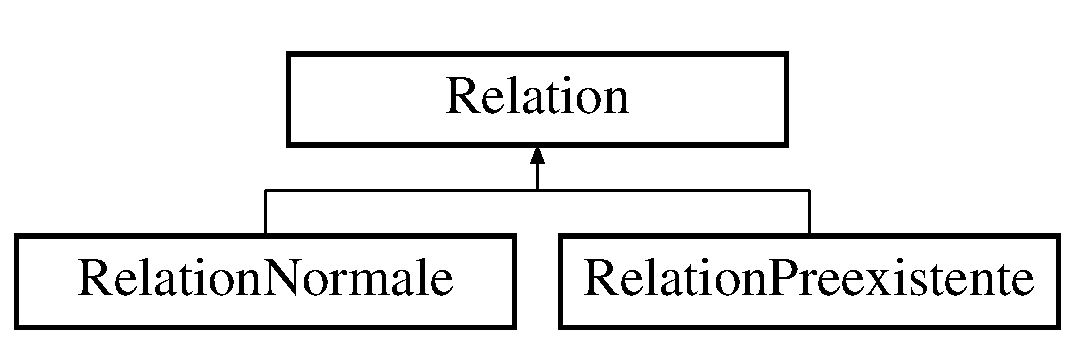
\includegraphics[height=2.000000cm]{class_relation}
\end{center}
\end{figure}
\subsection*{Classes}
\begin{DoxyCompactItemize}
\item 
class \hyperlink{class_relation_1_1iterator}{iterator}
\begin{DoxyCompactList}\small\item\em The iterator class\+: iterator of relation, iterate throught the table of couple. \end{DoxyCompactList}\end{DoxyCompactItemize}
\subsection*{Public Member Functions}
\begin{DoxyCompactItemize}
\item 
\hyperlink{class_relation_a2e93c9b24ab0748753655bdceb523d68}{Relation} (const Q\+String \&titr, const Q\+String \&desc=\char`\"{}\char`\"{}, bool orie=true)
\begin{DoxyCompactList}\small\item\em \hyperlink{class_relation}{Relation}\+: constructor of relation. \end{DoxyCompactList}\item 
virtual void \hyperlink{class_relation_a1c08a802796f5fccaa5732ec1a96e542}{set\+Titre} (const Q\+String \&new\+Titre)=0
\begin{DoxyCompactList}\small\item\em set\+Titre\+: set new titre \end{DoxyCompactList}\item 
virtual void \hyperlink{class_relation_a8f698cc45c38a849c4bcd8336fa5e2b3}{set\+Description} (const Q\+String \&new\+Description)=0
\begin{DoxyCompactList}\small\item\em set\+Description\+: set new description \end{DoxyCompactList}\item 
virtual void \hyperlink{class_relation_a5c93cf0ba3f16e75b83f3683b5ac26ec}{set\+Orientee} (bool bool\+Val)=0
\begin{DoxyCompactList}\small\item\em set\+Orientee\+: set new orientee \end{DoxyCompactList}\item 
const Q\+String \& \hyperlink{class_relation_a411be3a1dfc417342db768555a2afe41}{get\+Titre} () const
\begin{DoxyCompactList}\small\item\em get\+Titre\+: get titre of relation \end{DoxyCompactList}\item 
const Q\+String \& \hyperlink{class_relation_a078c6c43b163152aa40a9ac535175b9e}{get\+Description} () const
\begin{DoxyCompactList}\small\item\em get\+Description\+: get description of relation \end{DoxyCompactList}\item 
bool \hyperlink{class_relation_a4a985197f794d8f2d0c9a6d21c2eae13}{get\+Orientee} () const
\begin{DoxyCompactList}\small\item\em get\+Orientee\+: get orientee of relation \end{DoxyCompactList}\item 
void \hyperlink{class_relation_a9209a870df1bf2fc04e3803b3432cae7}{ajouter\+Couple} (\hyperlink{class_couple}{Couple} $\ast$new\+Couple)
\begin{DoxyCompactList}\small\item\em ajouter\+Couple\+: add new couple into relation \end{DoxyCompactList}\item 
void \hyperlink{class_relation_ac8e3f82f4d5afc302b4ee0f1641ba548}{supprimer\+Couple} (\hyperlink{class_couple}{Couple} $\ast$sup\+Couple)
\begin{DoxyCompactList}\small\item\em supprimer\+Couple\+: delete the couple \end{DoxyCompactList}\item 
virtual \hyperlink{class_relation_aac587ec926df3043c3eedcb5123be50b}{$\sim$\+Relation} ()
\begin{DoxyCompactList}\small\item\em $\sim$\+Relation\+: destructor of relation \end{DoxyCompactList}\item 
\hyperlink{class_relation_1_1iterator}{iterator} \hyperlink{class_relation_aa436b19e8361edc4de25b7b30b3bd010}{begin} ()
\begin{DoxyCompactList}\small\item\em begin\+: get the pointer to the beginning of the table of couple \end{DoxyCompactList}\item 
\hyperlink{class_relation_1_1iterator}{iterator} \hyperlink{class_relation_aee4ecfac883dc307d257d6976e7a191b}{end} ()
\begin{DoxyCompactList}\small\item\em end\+: get the pointer to the end of the table of couple \end{DoxyCompactList}\end{DoxyCompactItemize}
\subsection*{Protected Attributes}
\begin{DoxyCompactItemize}
\item 
\mbox{\Hypertarget{class_relation_a346e9b10df6757dee8dc13cb2f876357}\label{class_relation_a346e9b10df6757dee8dc13cb2f876357}} 
Q\+String \hyperlink{class_relation_a346e9b10df6757dee8dc13cb2f876357}{titre}
\begin{DoxyCompactList}\small\item\em titre\+: titre of the relation \end{DoxyCompactList}\item 
\mbox{\Hypertarget{class_relation_a1140829291bd04a86d0b840524692703}\label{class_relation_a1140829291bd04a86d0b840524692703}} 
Q\+String \hyperlink{class_relation_a1140829291bd04a86d0b840524692703}{description}
\begin{DoxyCompactList}\small\item\em description\+: description of the relation \end{DoxyCompactList}\item 
\mbox{\Hypertarget{class_relation_a1fb045a9e851d6989310ac89f5addc80}\label{class_relation_a1fb045a9e851d6989310ac89f5addc80}} 
bool \hyperlink{class_relation_a1fb045a9e851d6989310ac89f5addc80}{orientee}
\begin{DoxyCompactList}\small\item\em orientee\+: true if orientee \end{DoxyCompactList}\end{DoxyCompactItemize}


\subsection{Detailed Description}
The \hyperlink{class_relation}{Relation} class is abstract, it contains couples and the orientation of the couples inside. 

There are \hyperlink{class_relation_normale}{Relation\+Normale} and Relation\+Preexistence are inherit relation 

\subsection{Constructor \& Destructor Documentation}
\mbox{\Hypertarget{class_relation_a2e93c9b24ab0748753655bdceb523d68}\label{class_relation_a2e93c9b24ab0748753655bdceb523d68}} 
\index{Relation@{Relation}!Relation@{Relation}}
\index{Relation@{Relation}!Relation@{Relation}}
\subsubsection{\texorpdfstring{Relation()}{Relation()}}
{\footnotesize\ttfamily Relation\+::\+Relation (\begin{DoxyParamCaption}\item[{const Q\+String \&}]{titr,  }\item[{const Q\+String \&}]{desc = {\ttfamily \char`\"{}\char`\"{}},  }\item[{bool}]{orie = {\ttfamily true} }\end{DoxyParamCaption})\hspace{0.3cm}{\ttfamily [inline]}}



\hyperlink{class_relation}{Relation}\+: constructor of relation. 


\begin{DoxyParams}{Parameters}
{\em titr} & titre of the relation \\
\hline
{\em desc} & description of the relation \\
\hline
{\em orie} & orientation of the relation \\
\hline
\end{DoxyParams}
\mbox{\Hypertarget{class_relation_aac587ec926df3043c3eedcb5123be50b}\label{class_relation_aac587ec926df3043c3eedcb5123be50b}} 
\index{Relation@{Relation}!````~Relation@{$\sim$\+Relation}}
\index{````~Relation@{$\sim$\+Relation}!Relation@{Relation}}
\subsubsection{\texorpdfstring{$\sim$\+Relation()}{~Relation()}}
{\footnotesize\ttfamily virtual Relation\+::$\sim$\+Relation (\begin{DoxyParamCaption}{ }\end{DoxyParamCaption})\hspace{0.3cm}{\ttfamily [inline]}, {\ttfamily [virtual]}}



$\sim$\+Relation\+: destructor of relation 

Free the table couple, virtual function 

\subsection{Member Function Documentation}
\mbox{\Hypertarget{class_relation_a9209a870df1bf2fc04e3803b3432cae7}\label{class_relation_a9209a870df1bf2fc04e3803b3432cae7}} 
\index{Relation@{Relation}!ajouter\+Couple@{ajouter\+Couple}}
\index{ajouter\+Couple@{ajouter\+Couple}!Relation@{Relation}}
\subsubsection{\texorpdfstring{ajouter\+Couple()}{ajouterCouple()}}
{\footnotesize\ttfamily void Relation\+::ajouter\+Couple (\begin{DoxyParamCaption}\item[{\hyperlink{class_couple}{Couple} $\ast$}]{new\+Couple }\end{DoxyParamCaption})}



ajouter\+Couple\+: add new couple into relation 


\begin{DoxyParams}{Parameters}
{\em new\+Couple} & pointer to the new couple \\
\hline
\end{DoxyParams}
\mbox{\Hypertarget{class_relation_aa436b19e8361edc4de25b7b30b3bd010}\label{class_relation_aa436b19e8361edc4de25b7b30b3bd010}} 
\index{Relation@{Relation}!begin@{begin}}
\index{begin@{begin}!Relation@{Relation}}
\subsubsection{\texorpdfstring{begin()}{begin()}}
{\footnotesize\ttfamily \hyperlink{class_relation_1_1iterator}{iterator} Relation\+::begin (\begin{DoxyParamCaption}{ }\end{DoxyParamCaption})\hspace{0.3cm}{\ttfamily [inline]}}



begin\+: get the pointer to the beginning of the table of couple 

\begin{DoxyReturn}{Returns}
iterator 
\end{DoxyReturn}
\mbox{\Hypertarget{class_relation_aee4ecfac883dc307d257d6976e7a191b}\label{class_relation_aee4ecfac883dc307d257d6976e7a191b}} 
\index{Relation@{Relation}!end@{end}}
\index{end@{end}!Relation@{Relation}}
\subsubsection{\texorpdfstring{end()}{end()}}
{\footnotesize\ttfamily \hyperlink{class_relation_1_1iterator}{iterator} Relation\+::end (\begin{DoxyParamCaption}{ }\end{DoxyParamCaption})\hspace{0.3cm}{\ttfamily [inline]}}



end\+: get the pointer to the end of the table of couple 

\begin{DoxyReturn}{Returns}
iterator 
\end{DoxyReturn}
\mbox{\Hypertarget{class_relation_a078c6c43b163152aa40a9ac535175b9e}\label{class_relation_a078c6c43b163152aa40a9ac535175b9e}} 
\index{Relation@{Relation}!get\+Description@{get\+Description}}
\index{get\+Description@{get\+Description}!Relation@{Relation}}
\subsubsection{\texorpdfstring{get\+Description()}{getDescription()}}
{\footnotesize\ttfamily const Q\+String\& Relation\+::get\+Description (\begin{DoxyParamCaption}{ }\end{DoxyParamCaption}) const\hspace{0.3cm}{\ttfamily [inline]}}



get\+Description\+: get description of relation 

\begin{DoxyReturn}{Returns}
const Q\+String\& 
\end{DoxyReturn}
\mbox{\Hypertarget{class_relation_a4a985197f794d8f2d0c9a6d21c2eae13}\label{class_relation_a4a985197f794d8f2d0c9a6d21c2eae13}} 
\index{Relation@{Relation}!get\+Orientee@{get\+Orientee}}
\index{get\+Orientee@{get\+Orientee}!Relation@{Relation}}
\subsubsection{\texorpdfstring{get\+Orientee()}{getOrientee()}}
{\footnotesize\ttfamily bool Relation\+::get\+Orientee (\begin{DoxyParamCaption}{ }\end{DoxyParamCaption}) const\hspace{0.3cm}{\ttfamily [inline]}}



get\+Orientee\+: get orientee of relation 

\begin{DoxyReturn}{Returns}
bool 
\end{DoxyReturn}
\mbox{\Hypertarget{class_relation_a411be3a1dfc417342db768555a2afe41}\label{class_relation_a411be3a1dfc417342db768555a2afe41}} 
\index{Relation@{Relation}!get\+Titre@{get\+Titre}}
\index{get\+Titre@{get\+Titre}!Relation@{Relation}}
\subsubsection{\texorpdfstring{get\+Titre()}{getTitre()}}
{\footnotesize\ttfamily const Q\+String\& Relation\+::get\+Titre (\begin{DoxyParamCaption}{ }\end{DoxyParamCaption}) const\hspace{0.3cm}{\ttfamily [inline]}}



get\+Titre\+: get titre of relation 

\begin{DoxyReturn}{Returns}
const Q\+String\& 
\end{DoxyReturn}
\mbox{\Hypertarget{class_relation_a8f698cc45c38a849c4bcd8336fa5e2b3}\label{class_relation_a8f698cc45c38a849c4bcd8336fa5e2b3}} 
\index{Relation@{Relation}!set\+Description@{set\+Description}}
\index{set\+Description@{set\+Description}!Relation@{Relation}}
\subsubsection{\texorpdfstring{set\+Description()}{setDescription()}}
{\footnotesize\ttfamily virtual void Relation\+::set\+Description (\begin{DoxyParamCaption}\item[{const Q\+String \&}]{new\+Description }\end{DoxyParamCaption})\hspace{0.3cm}{\ttfamily [pure virtual]}}



set\+Description\+: set new description 


\begin{DoxyParams}{Parameters}
{\em new\+Description} & new description of the relation\\
\hline
\end{DoxyParams}
class pure virtual 

Implemented in \hyperlink{class_relation_normale_a74c586177c06279726df02dd1d8b721a}{Relation\+Normale}.

\mbox{\Hypertarget{class_relation_a5c93cf0ba3f16e75b83f3683b5ac26ec}\label{class_relation_a5c93cf0ba3f16e75b83f3683b5ac26ec}} 
\index{Relation@{Relation}!set\+Orientee@{set\+Orientee}}
\index{set\+Orientee@{set\+Orientee}!Relation@{Relation}}
\subsubsection{\texorpdfstring{set\+Orientee()}{setOrientee()}}
{\footnotesize\ttfamily virtual void Relation\+::set\+Orientee (\begin{DoxyParamCaption}\item[{bool}]{bool\+Val }\end{DoxyParamCaption})\hspace{0.3cm}{\ttfamily [pure virtual]}}



set\+Orientee\+: set new orientee 


\begin{DoxyParams}{Parameters}
{\em bool\+Val} & true if the relation is oriented\\
\hline
\end{DoxyParams}
class pure virtual 

Implemented in \hyperlink{class_relation_normale_a6095c88468d08fbe6c3d35fa5aedc635}{Relation\+Normale}.

\mbox{\Hypertarget{class_relation_a1c08a802796f5fccaa5732ec1a96e542}\label{class_relation_a1c08a802796f5fccaa5732ec1a96e542}} 
\index{Relation@{Relation}!set\+Titre@{set\+Titre}}
\index{set\+Titre@{set\+Titre}!Relation@{Relation}}
\subsubsection{\texorpdfstring{set\+Titre()}{setTitre()}}
{\footnotesize\ttfamily virtual void Relation\+::set\+Titre (\begin{DoxyParamCaption}\item[{const Q\+String \&}]{new\+Titre }\end{DoxyParamCaption})\hspace{0.3cm}{\ttfamily [pure virtual]}}



set\+Titre\+: set new titre 


\begin{DoxyParams}{Parameters}
{\em new\+Titre} & new titre of the relation\\
\hline
\end{DoxyParams}
class pure virtual 

Implemented in \hyperlink{class_relation_normale_abd0076a23f702ced9af181a0f046652c}{Relation\+Normale}.

\mbox{\Hypertarget{class_relation_ac8e3f82f4d5afc302b4ee0f1641ba548}\label{class_relation_ac8e3f82f4d5afc302b4ee0f1641ba548}} 
\index{Relation@{Relation}!supprimer\+Couple@{supprimer\+Couple}}
\index{supprimer\+Couple@{supprimer\+Couple}!Relation@{Relation}}
\subsubsection{\texorpdfstring{supprimer\+Couple()}{supprimerCouple()}}
{\footnotesize\ttfamily void Relation\+::supprimer\+Couple (\begin{DoxyParamCaption}\item[{\hyperlink{class_couple}{Couple} $\ast$}]{sup\+Couple }\end{DoxyParamCaption})}



supprimer\+Couple\+: delete the couple 


\begin{DoxyParams}{Parameters}
{\em sup\+Couple} & pointer to the couple need to delete \\
\hline
\end{DoxyParams}


The documentation for this class was generated from the following files\+:\begin{DoxyCompactItemize}
\item 
\hyperlink{relation_8h}{relation.\+h}\item 
relation.\+cpp\end{DoxyCompactItemize}

\hypertarget{class_relation_manager}{}\section{Relation\+Manager Class Reference}
\label{class_relation_manager}\index{Relation\+Manager@{Relation\+Manager}}


The \hyperlink{class_relation_manager}{Relation\+Manager} class\+: \hyperlink{class_relation}{Relation} Manager to manage \hyperlink{class_relation}{Relation}, Singleton.  




{\ttfamily \#include $<$relation.\+h$>$}

\subsection*{Classes}
\begin{DoxyCompactItemize}
\item 
class \hyperlink{class_relation_manager_1_1iterator}{iterator}
\begin{DoxyCompactList}\small\item\em The iterator class\+: iterator through table of relations. \end{DoxyCompactList}\end{DoxyCompactItemize}
\subsection*{Public Member Functions}
\begin{DoxyCompactItemize}
\item 
\hyperlink{class_relation}{Relation} $\ast$ \hyperlink{class_relation_manager_ab5eedc7d52a94e7377b532704366ee48}{get\+Relation\+From\+Title} (Q\+String \&title)
\begin{DoxyCompactList}\small\item\em get\+Relation\+From\+Title\+: return pointer to relation from a titre \end{DoxyCompactList}\item 
unsigned int \hyperlink{class_relation_manager_ac4f3ef3f86fd911fb6619de910a52411}{get\+Nb\+Relations} ()
\begin{DoxyCompactList}\small\item\em get\+Nb\+Relations\+: get number of relations in \hyperlink{class_relation_manager}{Relation\+Manager} \end{DoxyCompactList}\item 
void \hyperlink{class_relation_manager_a6661d400acae8992ce2d0677f7bb8bb7}{ajouter\+Relation} (\hyperlink{class_relation}{Relation} $\ast$new\+Relation)
\begin{DoxyCompactList}\small\item\em ajouter\+Relation\+: add \hyperlink{class_relation}{Relation} to table of \hyperlink{class_relation}{Relation} in \hyperlink{class_relation_manager}{Relation\+Manager} \end{DoxyCompactList}\item 
void \hyperlink{class_relation_manager_a1ab185cfa12b8632d44c7f705d0168f1}{supprimer\+Relation} (\hyperlink{class_relation}{Relation} $\ast$supprimer\+Relation)
\begin{DoxyCompactList}\small\item\em supprimer\+Relation\+: detete a \hyperlink{class_relation}{Relation} in \hyperlink{class_relation_manager}{Relation\+Manager} \end{DoxyCompactList}\item 
\hyperlink{class_relation_manager_1_1iterator}{iterator} \hyperlink{class_relation_manager_a0cbea7cf6799fb13153d1fab8b345487}{begin} ()
\begin{DoxyCompactList}\small\item\em begin\+: return the pointer to the first position in the table \end{DoxyCompactList}\item 
\hyperlink{class_relation_manager_1_1iterator}{iterator} \hyperlink{class_relation_manager_a9425308e362ee6921041d1e904785f19}{end} ()
\begin{DoxyCompactList}\small\item\em end\+: return the pointer to the end position in the table \end{DoxyCompactList}\item 
void \hyperlink{class_relation_manager_af587ffbf383d7fae096b0a2dba9ff679}{load\+Relation\+Manager} (const Q\+String \&filename)
\begin{DoxyCompactList}\small\item\em load\+Relation\+Manager\+: load .xml to \hyperlink{class_relation_manager}{Relation\+Manager} \end{DoxyCompactList}\item 
void \hyperlink{class_relation_manager_af12e8c983fdf15a3e84ec826c150fbea}{save\+Relation\+Manager} (const Q\+String \&filename)
\begin{DoxyCompactList}\small\item\em save\+Relation\+Manager\+: save \hyperlink{class_relation_manager}{Relation\+Manager} to .xml \end{DoxyCompactList}\end{DoxyCompactItemize}
\subsection*{Static Public Member Functions}
\begin{DoxyCompactItemize}
\item 
static \hyperlink{class_relation_manager}{Relation\+Manager} $\ast$ \hyperlink{class_relation_manager_a507b3edf840eb79a29f46662f3c30d04}{get\+Relation\+Manager} ()
\begin{DoxyCompactList}\small\item\em get\+Relation\+Manager\+: get instance of \hyperlink{class_relation_manager}{Relation\+Manager}, contruct if there is no instance of \hyperlink{class_relation_manager}{Relation\+Manager} \end{DoxyCompactList}\item 
\mbox{\Hypertarget{class_relation_manager_a9ba5983117f98b5bb83bd41575f736b9}\label{class_relation_manager_a9ba5983117f98b5bb83bd41575f736b9}} 
static void \hyperlink{class_relation_manager_a9ba5983117f98b5bb83bd41575f736b9}{liberer\+Relation\+Manager} ()
\begin{DoxyCompactList}\small\item\em liberer\+Relation\+Manager\+: Free the instance of \hyperlink{class_relation_manager}{Relation\+Manager} \end{DoxyCompactList}\end{DoxyCompactItemize}


\subsection{Detailed Description}
The \hyperlink{class_relation_manager}{Relation\+Manager} class\+: \hyperlink{class_relation}{Relation} Manager to manage \hyperlink{class_relation}{Relation}, Singleton. 

\subsection{Member Function Documentation}
\mbox{\Hypertarget{class_relation_manager_a6661d400acae8992ce2d0677f7bb8bb7}\label{class_relation_manager_a6661d400acae8992ce2d0677f7bb8bb7}} 
\index{Relation\+Manager@{Relation\+Manager}!ajouter\+Relation@{ajouter\+Relation}}
\index{ajouter\+Relation@{ajouter\+Relation}!Relation\+Manager@{Relation\+Manager}}
\subsubsection{\texorpdfstring{ajouter\+Relation()}{ajouterRelation()}}
{\footnotesize\ttfamily void Relation\+Manager\+::ajouter\+Relation (\begin{DoxyParamCaption}\item[{\hyperlink{class_relation}{Relation} $\ast$}]{new\+Relation }\end{DoxyParamCaption})}



ajouter\+Relation\+: add \hyperlink{class_relation}{Relation} to table of \hyperlink{class_relation}{Relation} in \hyperlink{class_relation_manager}{Relation\+Manager} 


\begin{DoxyParams}{Parameters}
{\em new\+Relation} & pointer to the new\+Relation \\
\hline
\end{DoxyParams}
\mbox{\Hypertarget{class_relation_manager_a0cbea7cf6799fb13153d1fab8b345487}\label{class_relation_manager_a0cbea7cf6799fb13153d1fab8b345487}} 
\index{Relation\+Manager@{Relation\+Manager}!begin@{begin}}
\index{begin@{begin}!Relation\+Manager@{Relation\+Manager}}
\subsubsection{\texorpdfstring{begin()}{begin()}}
{\footnotesize\ttfamily \hyperlink{class_relation_manager_1_1iterator}{iterator} Relation\+Manager\+::begin (\begin{DoxyParamCaption}{ }\end{DoxyParamCaption})\hspace{0.3cm}{\ttfamily [inline]}}



begin\+: return the pointer to the first position in the table 

\begin{DoxyReturn}{Returns}
iterator 
\end{DoxyReturn}
\mbox{\Hypertarget{class_relation_manager_a9425308e362ee6921041d1e904785f19}\label{class_relation_manager_a9425308e362ee6921041d1e904785f19}} 
\index{Relation\+Manager@{Relation\+Manager}!end@{end}}
\index{end@{end}!Relation\+Manager@{Relation\+Manager}}
\subsubsection{\texorpdfstring{end()}{end()}}
{\footnotesize\ttfamily \hyperlink{class_relation_manager_1_1iterator}{iterator} Relation\+Manager\+::end (\begin{DoxyParamCaption}{ }\end{DoxyParamCaption})\hspace{0.3cm}{\ttfamily [inline]}}



end\+: return the pointer to the end position in the table 

\begin{DoxyReturn}{Returns}
iterator 
\end{DoxyReturn}
\mbox{\Hypertarget{class_relation_manager_ac4f3ef3f86fd911fb6619de910a52411}\label{class_relation_manager_ac4f3ef3f86fd911fb6619de910a52411}} 
\index{Relation\+Manager@{Relation\+Manager}!get\+Nb\+Relations@{get\+Nb\+Relations}}
\index{get\+Nb\+Relations@{get\+Nb\+Relations}!Relation\+Manager@{Relation\+Manager}}
\subsubsection{\texorpdfstring{get\+Nb\+Relations()}{getNbRelations()}}
{\footnotesize\ttfamily unsigned int Relation\+Manager\+::get\+Nb\+Relations (\begin{DoxyParamCaption}{ }\end{DoxyParamCaption})\hspace{0.3cm}{\ttfamily [inline]}}



get\+Nb\+Relations\+: get number of relations in \hyperlink{class_relation_manager}{Relation\+Manager} 

\begin{DoxyReturn}{Returns}
unsigned int 
\end{DoxyReturn}
\mbox{\Hypertarget{class_relation_manager_ab5eedc7d52a94e7377b532704366ee48}\label{class_relation_manager_ab5eedc7d52a94e7377b532704366ee48}} 
\index{Relation\+Manager@{Relation\+Manager}!get\+Relation\+From\+Title@{get\+Relation\+From\+Title}}
\index{get\+Relation\+From\+Title@{get\+Relation\+From\+Title}!Relation\+Manager@{Relation\+Manager}}
\subsubsection{\texorpdfstring{get\+Relation\+From\+Title()}{getRelationFromTitle()}}
{\footnotesize\ttfamily \hyperlink{class_relation}{Relation} $\ast$ Relation\+Manager\+::get\+Relation\+From\+Title (\begin{DoxyParamCaption}\item[{Q\+String \&}]{title }\end{DoxyParamCaption})}



get\+Relation\+From\+Title\+: return pointer to relation from a titre 


\begin{DoxyParams}{Parameters}
{\em titre} & titre of the relation \\
\hline
\end{DoxyParams}
\begin{DoxyReturn}{Returns}
Relation$\ast$ 
\end{DoxyReturn}
\mbox{\Hypertarget{class_relation_manager_a507b3edf840eb79a29f46662f3c30d04}\label{class_relation_manager_a507b3edf840eb79a29f46662f3c30d04}} 
\index{Relation\+Manager@{Relation\+Manager}!get\+Relation\+Manager@{get\+Relation\+Manager}}
\index{get\+Relation\+Manager@{get\+Relation\+Manager}!Relation\+Manager@{Relation\+Manager}}
\subsubsection{\texorpdfstring{get\+Relation\+Manager()}{getRelationManager()}}
{\footnotesize\ttfamily static \hyperlink{class_relation_manager}{Relation\+Manager}$\ast$ Relation\+Manager\+::get\+Relation\+Manager (\begin{DoxyParamCaption}{ }\end{DoxyParamCaption})\hspace{0.3cm}{\ttfamily [inline]}, {\ttfamily [static]}}



get\+Relation\+Manager\+: get instance of \hyperlink{class_relation_manager}{Relation\+Manager}, contruct if there is no instance of \hyperlink{class_relation_manager}{Relation\+Manager} 

\begin{DoxyReturn}{Returns}
pointer to instance of \hyperlink{class_relation_manager}{Relation\+Manager} 
\end{DoxyReturn}
\mbox{\Hypertarget{class_relation_manager_af587ffbf383d7fae096b0a2dba9ff679}\label{class_relation_manager_af587ffbf383d7fae096b0a2dba9ff679}} 
\index{Relation\+Manager@{Relation\+Manager}!load\+Relation\+Manager@{load\+Relation\+Manager}}
\index{load\+Relation\+Manager@{load\+Relation\+Manager}!Relation\+Manager@{Relation\+Manager}}
\subsubsection{\texorpdfstring{load\+Relation\+Manager()}{loadRelationManager()}}
{\footnotesize\ttfamily void Relation\+Manager\+::load\+Relation\+Manager (\begin{DoxyParamCaption}\item[{const Q\+String \&}]{filename }\end{DoxyParamCaption})}



load\+Relation\+Manager\+: load .xml to \hyperlink{class_relation_manager}{Relation\+Manager} 


\begin{DoxyParams}{Parameters}
{\em filename} & file .xml to load \\
\hline
\end{DoxyParams}
\mbox{\Hypertarget{class_relation_manager_af12e8c983fdf15a3e84ec826c150fbea}\label{class_relation_manager_af12e8c983fdf15a3e84ec826c150fbea}} 
\index{Relation\+Manager@{Relation\+Manager}!save\+Relation\+Manager@{save\+Relation\+Manager}}
\index{save\+Relation\+Manager@{save\+Relation\+Manager}!Relation\+Manager@{Relation\+Manager}}
\subsubsection{\texorpdfstring{save\+Relation\+Manager()}{saveRelationManager()}}
{\footnotesize\ttfamily void Relation\+Manager\+::save\+Relation\+Manager (\begin{DoxyParamCaption}\item[{const Q\+String \&}]{filename }\end{DoxyParamCaption})}



save\+Relation\+Manager\+: save \hyperlink{class_relation_manager}{Relation\+Manager} to .xml 


\begin{DoxyParams}{Parameters}
{\em filename} & save to file .xml \\
\hline
\end{DoxyParams}
\mbox{\Hypertarget{class_relation_manager_a1ab185cfa12b8632d44c7f705d0168f1}\label{class_relation_manager_a1ab185cfa12b8632d44c7f705d0168f1}} 
\index{Relation\+Manager@{Relation\+Manager}!supprimer\+Relation@{supprimer\+Relation}}
\index{supprimer\+Relation@{supprimer\+Relation}!Relation\+Manager@{Relation\+Manager}}
\subsubsection{\texorpdfstring{supprimer\+Relation()}{supprimerRelation()}}
{\footnotesize\ttfamily void Relation\+Manager\+::supprimer\+Relation (\begin{DoxyParamCaption}\item[{\hyperlink{class_relation}{Relation} $\ast$}]{supprimer\+Relation }\end{DoxyParamCaption})}



supprimer\+Relation\+: detete a \hyperlink{class_relation}{Relation} in \hyperlink{class_relation_manager}{Relation\+Manager} 


\begin{DoxyParams}{Parameters}
{\em supprimer\+Relation} & pointer to the \hyperlink{class_relation}{Relation} needed to delete \\
\hline
\end{DoxyParams}


The documentation for this class was generated from the following files\+:\begin{DoxyCompactItemize}
\item 
\hyperlink{relation_8h}{relation.\+h}\item 
relation.\+cpp\end{DoxyCompactItemize}

\hypertarget{class_relation_normale}{}\section{Relation\+Normale Class Reference}
\label{class_relation_normale}\index{Relation\+Normale@{Relation\+Normale}}


The \hyperlink{class_relation_normale}{Relation\+Normale} class\+: heritate of \hyperlink{class_relation}{Relation} class.  




{\ttfamily \#include $<$relation.\+h$>$}

Inheritance diagram for Relation\+Normale\+:\begin{figure}[H]
\begin{center}
\leavevmode
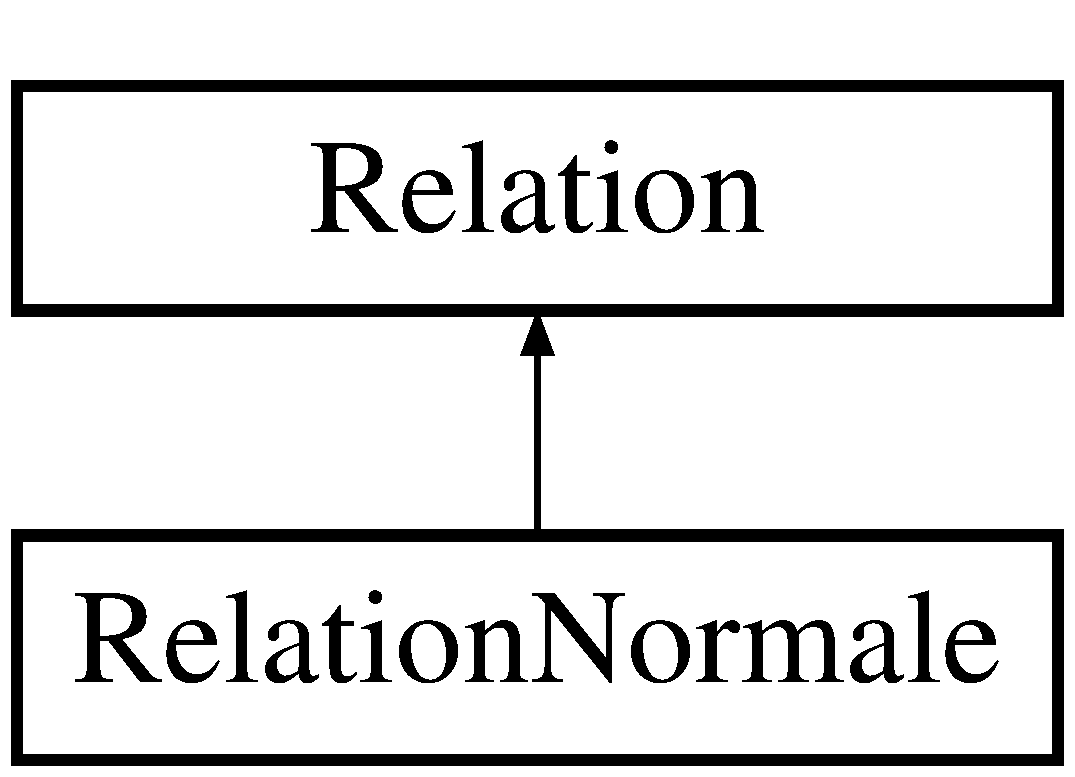
\includegraphics[height=2.000000cm]{class_relation_normale}
\end{center}
\end{figure}
\subsection*{Public Member Functions}
\begin{DoxyCompactItemize}
\item 
\hyperlink{class_relation_normale_a72d6b0c9f9e59ee634542aee57f2a9fb}{Relation\+Normale} (const Q\+String \&titr, const Q\+String \&desc, bool orie=true)
\begin{DoxyCompactList}\small\item\em \hyperlink{class_relation_normale}{Relation\+Normale}\+: constructor of \hyperlink{class_relation_normale}{Relation\+Normale}. \end{DoxyCompactList}\item 
void \hyperlink{class_relation_normale_abd0076a23f702ced9af181a0f046652c}{set\+Titre} (const Q\+String \&new\+Titre)
\begin{DoxyCompactList}\small\item\em set\+Titre\+: set new titre to \hyperlink{class_relation_normale}{Relation\+Normale} \end{DoxyCompactList}\item 
void \hyperlink{class_relation_normale_a74c586177c06279726df02dd1d8b721a}{set\+Description} (const Q\+String \&new\+Description)
\begin{DoxyCompactList}\small\item\em set\+Description\+: set new description to \hyperlink{class_relation_normale}{Relation\+Normale} \end{DoxyCompactList}\item 
void \hyperlink{class_relation_normale_a6095c88468d08fbe6c3d35fa5aedc635}{set\+Orientee} (bool bool\+Val)
\begin{DoxyCompactList}\small\item\em set\+Orientee\+: set new orientee to \hyperlink{class_relation_normale}{Relation\+Normale} \end{DoxyCompactList}\end{DoxyCompactItemize}
\subsection*{Additional Inherited Members}


\subsection{Detailed Description}
The \hyperlink{class_relation_normale}{Relation\+Normale} class\+: heritate of \hyperlink{class_relation}{Relation} class. 

Normal relation which can be deleted and change titre, description and orientation 

\subsection{Constructor \& Destructor Documentation}
\mbox{\Hypertarget{class_relation_normale_a72d6b0c9f9e59ee634542aee57f2a9fb}\label{class_relation_normale_a72d6b0c9f9e59ee634542aee57f2a9fb}} 
\index{Relation\+Normale@{Relation\+Normale}!Relation\+Normale@{Relation\+Normale}}
\index{Relation\+Normale@{Relation\+Normale}!Relation\+Normale@{Relation\+Normale}}
\subsubsection{\texorpdfstring{Relation\+Normale()}{RelationNormale()}}
{\footnotesize\ttfamily Relation\+Normale\+::\+Relation\+Normale (\begin{DoxyParamCaption}\item[{const Q\+String \&}]{titr,  }\item[{const Q\+String \&}]{desc,  }\item[{bool}]{orie = {\ttfamily true} }\end{DoxyParamCaption})\hspace{0.3cm}{\ttfamily [inline]}}



\hyperlink{class_relation_normale}{Relation\+Normale}\+: constructor of \hyperlink{class_relation_normale}{Relation\+Normale}. 


\begin{DoxyParams}{Parameters}
{\em titr} & titre of \hyperlink{class_relation_normale}{Relation\+Normale} \\
\hline
{\em desc} & description of \hyperlink{class_relation_normale}{Relation\+Normale} \\
\hline
{\em orie} & orientation of \hyperlink{class_relation_normale}{Relation\+Normale}, true if orientee \\
\hline
\end{DoxyParams}


\subsection{Member Function Documentation}
\mbox{\Hypertarget{class_relation_normale_a74c586177c06279726df02dd1d8b721a}\label{class_relation_normale_a74c586177c06279726df02dd1d8b721a}} 
\index{Relation\+Normale@{Relation\+Normale}!set\+Description@{set\+Description}}
\index{set\+Description@{set\+Description}!Relation\+Normale@{Relation\+Normale}}
\subsubsection{\texorpdfstring{set\+Description()}{setDescription()}}
{\footnotesize\ttfamily void Relation\+Normale\+::set\+Description (\begin{DoxyParamCaption}\item[{const Q\+String \&}]{new\+Description }\end{DoxyParamCaption})\hspace{0.3cm}{\ttfamily [inline]}, {\ttfamily [virtual]}}



set\+Description\+: set new description to \hyperlink{class_relation_normale}{Relation\+Normale} 


\begin{DoxyParams}{Parameters}
{\em new\+Description} & new description of \hyperlink{class_relation_normale}{Relation\+Normale} \\
\hline
\end{DoxyParams}


Implements \hyperlink{class_relation_a8f698cc45c38a849c4bcd8336fa5e2b3}{Relation}.

\mbox{\Hypertarget{class_relation_normale_a6095c88468d08fbe6c3d35fa5aedc635}\label{class_relation_normale_a6095c88468d08fbe6c3d35fa5aedc635}} 
\index{Relation\+Normale@{Relation\+Normale}!set\+Orientee@{set\+Orientee}}
\index{set\+Orientee@{set\+Orientee}!Relation\+Normale@{Relation\+Normale}}
\subsubsection{\texorpdfstring{set\+Orientee()}{setOrientee()}}
{\footnotesize\ttfamily void Relation\+Normale\+::set\+Orientee (\begin{DoxyParamCaption}\item[{bool}]{bool\+Val }\end{DoxyParamCaption})\hspace{0.3cm}{\ttfamily [inline]}, {\ttfamily [virtual]}}



set\+Orientee\+: set new orientee to \hyperlink{class_relation_normale}{Relation\+Normale} 


\begin{DoxyParams}{Parameters}
{\em bool\+Val} & true of orientee \\
\hline
\end{DoxyParams}


Implements \hyperlink{class_relation_a5c93cf0ba3f16e75b83f3683b5ac26ec}{Relation}.

\mbox{\Hypertarget{class_relation_normale_abd0076a23f702ced9af181a0f046652c}\label{class_relation_normale_abd0076a23f702ced9af181a0f046652c}} 
\index{Relation\+Normale@{Relation\+Normale}!set\+Titre@{set\+Titre}}
\index{set\+Titre@{set\+Titre}!Relation\+Normale@{Relation\+Normale}}
\subsubsection{\texorpdfstring{set\+Titre()}{setTitre()}}
{\footnotesize\ttfamily void Relation\+Normale\+::set\+Titre (\begin{DoxyParamCaption}\item[{const Q\+String \&}]{new\+Titre }\end{DoxyParamCaption})\hspace{0.3cm}{\ttfamily [inline]}, {\ttfamily [virtual]}}



set\+Titre\+: set new titre to \hyperlink{class_relation_normale}{Relation\+Normale} 


\begin{DoxyParams}{Parameters}
{\em new\+Titre} & new titre of \hyperlink{class_relation_normale}{Relation\+Normale} \\
\hline
\end{DoxyParams}


Implements \hyperlink{class_relation_a1c08a802796f5fccaa5732ec1a96e542}{Relation}.



The documentation for this class was generated from the following file\+:\begin{DoxyCompactItemize}
\item 
\hyperlink{relation_8h}{relation.\+h}\end{DoxyCompactItemize}

\hypertarget{class_relation_preexistente}{}\section{Relation\+Preexistente Class Reference}
\label{class_relation_preexistente}\index{Relation\+Preexistente@{Relation\+Preexistente}}


The \hyperlink{class_relation_preexistente}{Relation\+Preexistente} class\+: the Preexistence class, Reference.  




{\ttfamily \#include $<$relation.\+h$>$}

Inheritance diagram for Relation\+Preexistente\+:\begin{figure}[H]
\begin{center}
\leavevmode
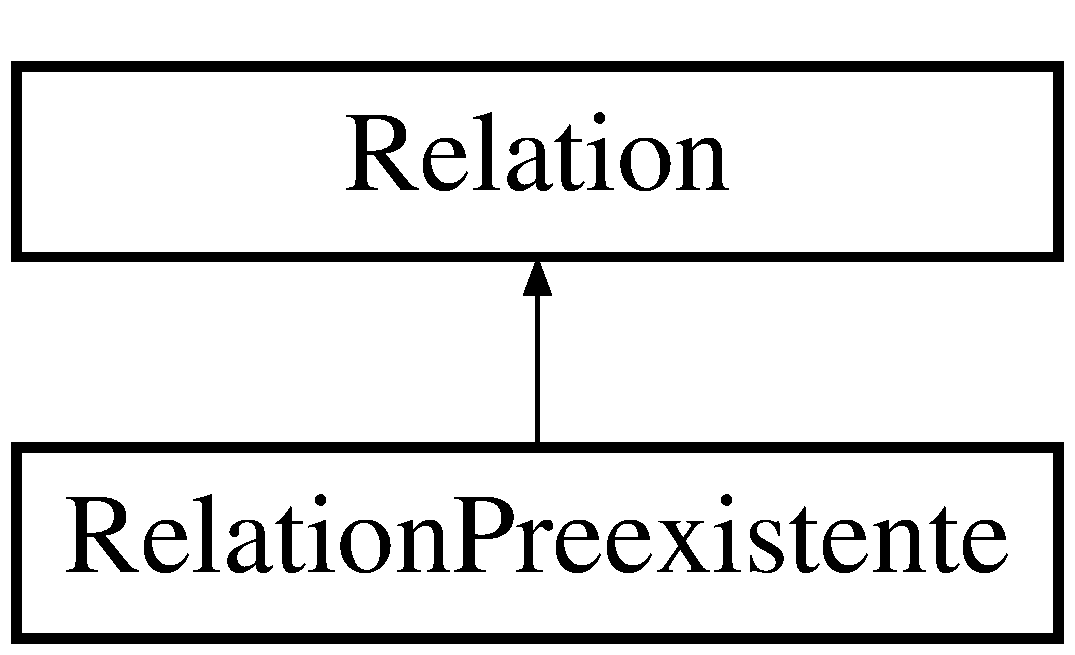
\includegraphics[height=2.000000cm]{class_relation_preexistente}
\end{center}
\end{figure}
\subsection*{Static Public Member Functions}
\begin{DoxyCompactItemize}
\item 
static \hyperlink{class_relation_preexistente}{Relation\+Preexistente} $\ast$ \hyperlink{class_relation_preexistente_afd2c7ee8104d9dee00b52e5af1f5ed59}{get\+Relation\+Preexistente} ()
\begin{DoxyCompactList}\small\item\em get\+Relation\+Preexistente\+: get the Relation\+Preexistence \end{DoxyCompactList}\item 
\mbox{\Hypertarget{class_relation_preexistente_ab6d6d23dc7edfb6773c56ffad69baf8f}\label{class_relation_preexistente_ab6d6d23dc7edfb6773c56ffad69baf8f}} 
static void {\bfseries liberer\+Relation\+Preexistente} ()
\end{DoxyCompactItemize}
\subsection*{Additional Inherited Members}


\subsection{Detailed Description}
The \hyperlink{class_relation_preexistente}{Relation\+Preexistente} class\+: the Preexistence class, Reference. 

Cannot delete this class, this class hold the first place in table of \hyperlink{class_relation}{Relation} in \hyperlink{class_relation_manager}{Relation\+Manager}, singleton 

\subsection{Member Function Documentation}
\mbox{\Hypertarget{class_relation_preexistente_afd2c7ee8104d9dee00b52e5af1f5ed59}\label{class_relation_preexistente_afd2c7ee8104d9dee00b52e5af1f5ed59}} 
\index{Relation\+Preexistente@{Relation\+Preexistente}!get\+Relation\+Preexistente@{get\+Relation\+Preexistente}}
\index{get\+Relation\+Preexistente@{get\+Relation\+Preexistente}!Relation\+Preexistente@{Relation\+Preexistente}}
\subsubsection{\texorpdfstring{get\+Relation\+Preexistente()}{getRelationPreexistente()}}
{\footnotesize\ttfamily static \hyperlink{class_relation_preexistente}{Relation\+Preexistente}$\ast$ Relation\+Preexistente\+::get\+Relation\+Preexistente (\begin{DoxyParamCaption}{ }\end{DoxyParamCaption})\hspace{0.3cm}{\ttfamily [inline]}, {\ttfamily [static]}}



get\+Relation\+Preexistente\+: get the Relation\+Preexistence 

\begin{DoxyReturn}{Returns}
the instance of Relation\+Preexistence
\end{DoxyReturn}
contruct new instance if there is no instance, otherwise get the instance pointer 

The documentation for this class was generated from the following files\+:\begin{DoxyCompactItemize}
\item 
\hyperlink{relation_8h}{relation.\+h}\item 
relation.\+cpp\end{DoxyCompactItemize}

\hypertarget{class_tache}{}\section{Tache Class Reference}
\label{class_tache}\index{Tache@{Tache}}


Définit la classe \hyperlink{class_tache}{Tache}.  




{\ttfamily \#include $<$tache.\+h$>$}

Inheritance diagram for Tache\+:\begin{figure}[H]
\begin{center}
\leavevmode
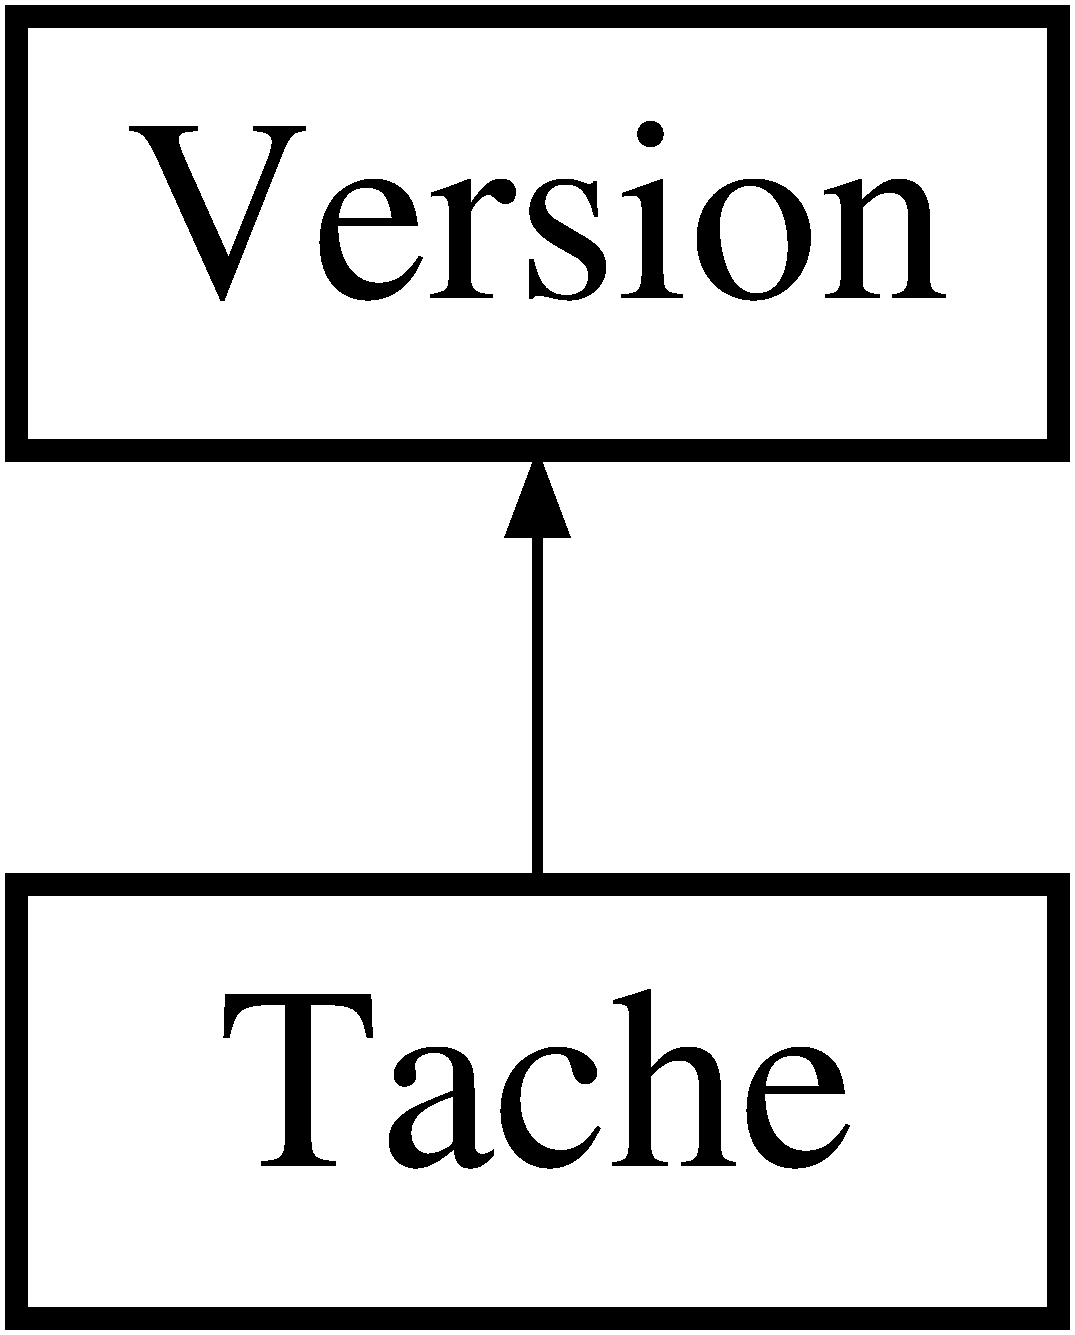
\includegraphics[height=2.000000cm]{class_tache}
\end{center}
\end{figure}
\subsection*{Public Member Functions}
\begin{DoxyCompactItemize}
\item 
\mbox{\Hypertarget{class_tache_aff51aaa66ab5616767b8bcb8ba6efb66}\label{class_tache_aff51aaa66ab5616767b8bcb8ba6efb66}} 
{\bfseries Tache} (const Q\+String \&t, Q\+Date\+Time d, const Q\+String \&a, const \hyperlink{tache_8h_addeb79f2c3a0b32730bfe5fe5eb962a7}{Type\+\_\+statut\+\_\+tache} \&s=attente)
\item 
\mbox{\Hypertarget{class_tache_aafda12978303cd10a514031bdc0bce0c}\label{class_tache_aafda12978303cd10a514031bdc0bce0c}} 
Q\+String {\bfseries get\+Action} () const
\item 
\mbox{\Hypertarget{class_tache_ad7f5a2ad90ada488f24f6d110e962d93}\label{class_tache_ad7f5a2ad90ada488f24f6d110e962d93}} 
unsigned int {\bfseries get\+Priorite} () const
\item 
\mbox{\Hypertarget{class_tache_a7ea3d62ae653087aca773a60572776e1}\label{class_tache_a7ea3d62ae653087aca773a60572776e1}} 
Q\+Date\+Time {\bfseries get\+Date\+\_\+echeance} () const
\item 
\mbox{\Hypertarget{class_tache_a85315e9a77532eaee87dbda30d3caa7c}\label{class_tache_a85315e9a77532eaee87dbda30d3caa7c}} 
\hyperlink{tache_8h_addeb79f2c3a0b32730bfe5fe5eb962a7}{Type\+\_\+statut\+\_\+tache} {\bfseries get\+Statut} () const
\item 
\mbox{\Hypertarget{class_tache_aec909e1855f0553610f191c395412367}\label{class_tache_aec909e1855f0553610f191c395412367}} 
void {\bfseries set\+Action} (const Q\+String new\+Action)
\item 
\mbox{\Hypertarget{class_tache_a1fa817dc840ff1c43bd6dba95ed14482}\label{class_tache_a1fa817dc840ff1c43bd6dba95ed14482}} 
void {\bfseries set\+Priorite} (const unsigned int new\+Priorite)
\item 
\mbox{\Hypertarget{class_tache_a01326a5425dee88e3fb727ab9c823a7f}\label{class_tache_a01326a5425dee88e3fb727ab9c823a7f}} 
void {\bfseries set\+Date\+\_\+echeance} (Q\+Date\+Time \&new\+Date)
\item 
\mbox{\Hypertarget{class_tache_a323fc789b8e715472f0947e74213b859}\label{class_tache_a323fc789b8e715472f0947e74213b859}} 
void {\bfseries set\+Statut} (const \hyperlink{tache_8h_addeb79f2c3a0b32730bfe5fe5eb962a7}{Type\+\_\+statut\+\_\+tache} \&new\+Statut)
\end{DoxyCompactItemize}


\subsection{Detailed Description}
Définit la classe \hyperlink{class_tache}{Tache}. 

Hérite de {\bfseries \hyperlink{class_version}{Version}} {\itshape action} \+: Action de la tâche {\itshape statut} \+: Statut de la tâche {\itshape priorite} \+: Priorité de la tâche (optionnelle) {\itshape date\+\_\+echeance} \+: date d\textquotesingle{}échaance de la tâche (optionnelle) 

The documentation for this class was generated from the following file\+:\begin{DoxyCompactItemize}
\item 
\hyperlink{tache_8h}{tache.\+h}\end{DoxyCompactItemize}

\hypertarget{class_template}{}\section{Template Class Reference}
\label{class_template}\index{Template@{Template}}


\subsection{Detailed Description}
la classe \hyperlink{class_iterator}{Iterator} sur une note 

The documentation for this class was generated from the following file\+:\begin{DoxyCompactItemize}
\item 
\hyperlink{notesmanager_8h}{notesmanager.\+h}\end{DoxyCompactItemize}

\hypertarget{class_template}{}\section{Template Class Reference}
\label{class_template}\index{Template@{Template}}


\subsection{Detailed Description}
la classe \hyperlink{class_iterator}{Iterator} sur une note 

The documentation for this class was generated from the following file\+:\begin{DoxyCompactItemize}
\item 
\hyperlink{notesmanager_8h}{notesmanager.\+h}\end{DoxyCompactItemize}

\hypertarget{class_version}{}\section{Version Class Reference}
\label{class_version}\index{Version@{Version}}


Définit la classe \hyperlink{class_version}{Version}.  




{\ttfamily \#include $<$version.\+h$>$}

Inheritance diagram for Version\+:\begin{figure}[H]
\begin{center}
\leavevmode
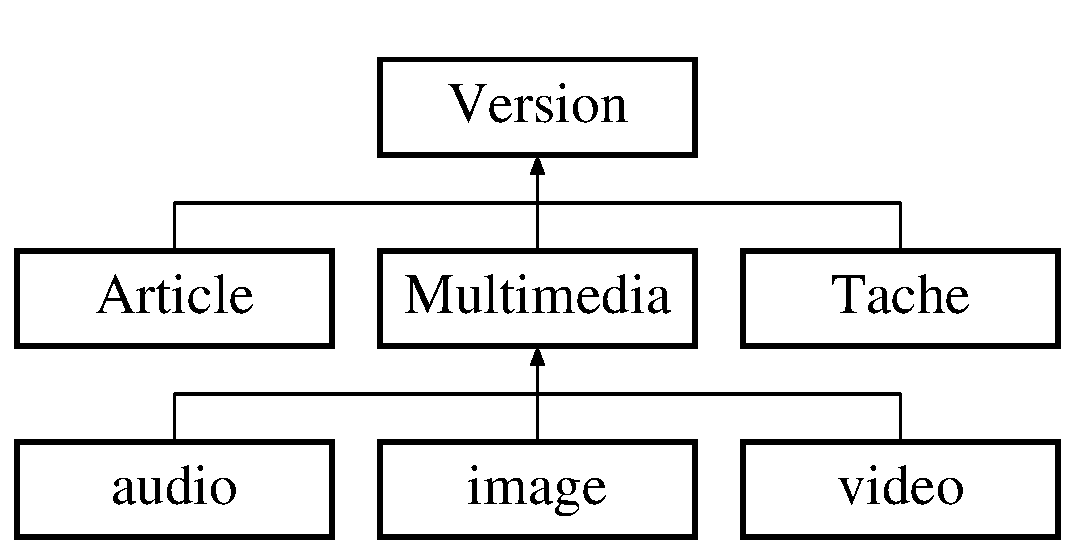
\includegraphics[height=3.000000cm]{class_version}
\end{center}
\end{figure}
\subsection*{Public Member Functions}
\begin{DoxyCompactItemize}
\item 
\mbox{\Hypertarget{class_version_ab48e595b9f0ed6ef7048048eb0dd537d}\label{class_version_ab48e595b9f0ed6ef7048048eb0dd537d}} 
{\bfseries Version} (const Q\+String \&t, const Q\+Date\+Time \&d)
\item 
\mbox{\Hypertarget{class_version_a54015f35fb47dea6e46e47ad9f8555ae}\label{class_version_a54015f35fb47dea6e46e47ad9f8555ae}} 
virtual Q\+String {\bfseries get\+Title} () const
\item 
\mbox{\Hypertarget{class_version_a757be3ac49f4a28f91bebb14d00cfe9a}\label{class_version_a757be3ac49f4a28f91bebb14d00cfe9a}} 
virtual Q\+Date\+Time {\bfseries get\+Date\+Modif} () const
\item 
\mbox{\Hypertarget{class_version_ae85b36ab74d00d8dc8fa88ef5ccb3c20}\label{class_version_ae85b36ab74d00d8dc8fa88ef5ccb3c20}} 
virtual void {\bfseries set\+Title} (const Q\+String \&new\+Title)
\item 
\mbox{\Hypertarget{class_version_a925ae5cb79c371a278e7bfd5a3b094a2}\label{class_version_a925ae5cb79c371a278e7bfd5a3b094a2}} 
virtual void {\bfseries set\+Date} (const Q\+Date\+Time \&new\+Date)
\end{DoxyCompactItemize}


\subsection{Detailed Description}
Définit la classe \hyperlink{class_version}{Version}. 

Classe abstraite {\itshape title} \+: Titre {\itshape date\+\_\+modif} \+: Date de dernière modification 

The documentation for this class was generated from the following files\+:\begin{DoxyCompactItemize}
\item 
\hyperlink{version_8h}{version.\+h}\item 
version.\+cpp\end{DoxyCompactItemize}

\hypertarget{classvideo}{}\section{video Class Reference}
\label{classvideo}\index{video@{video}}


Classe video hérite de \hyperlink{class_multimedia}{Multimedia}.  




{\ttfamily \#include $<$multimedia.\+h$>$}

Inheritance diagram for video\+:\begin{figure}[H]
\begin{center}
\leavevmode
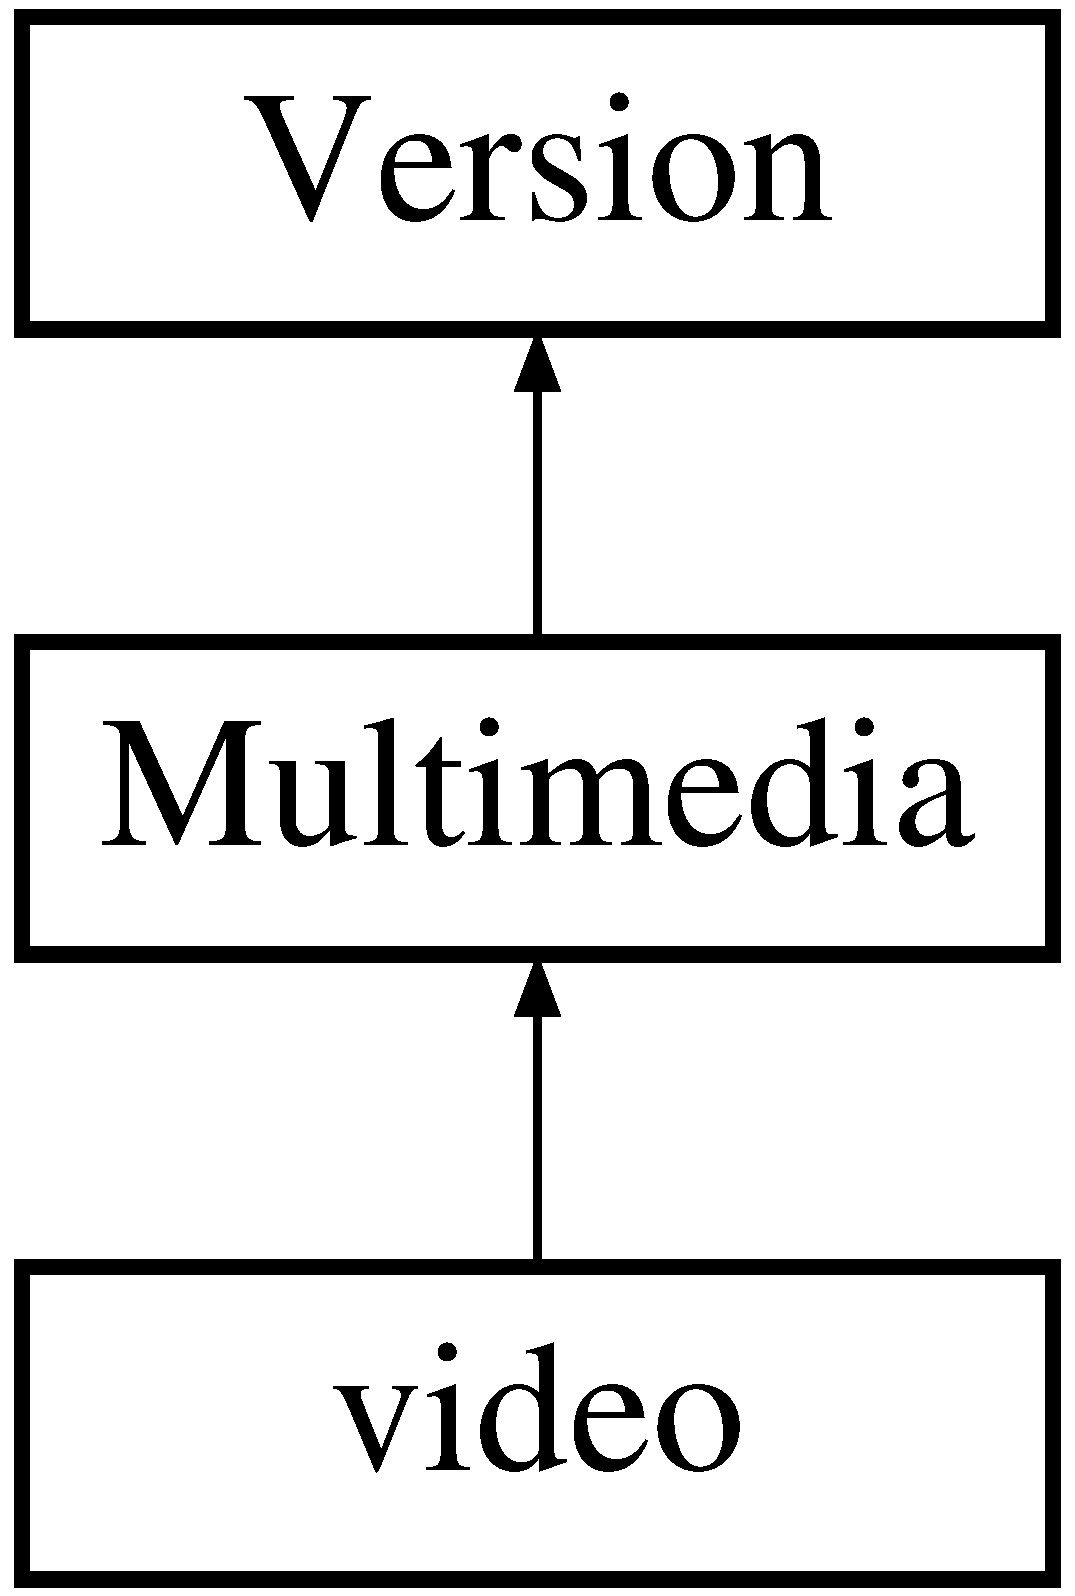
\includegraphics[height=3.000000cm]{classvideo}
\end{center}
\end{figure}
\subsection*{Public Member Functions}
\begin{DoxyCompactItemize}
\item 
\mbox{\Hypertarget{classvideo_a2a591da294b0c93de60d1241b1452d50}\label{classvideo_a2a591da294b0c93de60d1241b1452d50}} 
{\bfseries video} (const Q\+String \&t, Q\+Date\+Time d, const Q\+String \&desc, const Q\+String \&i, Q\+String vid)
\item 
\mbox{\Hypertarget{classvideo_a1b68b660607eb3a0a0293e44ffdcf467}\label{classvideo_a1b68b660607eb3a0a0293e44ffdcf467}} 
const Q\+String \& {\bfseries get\+Video\+\_\+\+U\+RL} () const
\item 
void \hyperlink{classvideo_a557dedaa9915167c5a4ad1eacc9c8a27}{play\+Video} () const
\item 
void \hyperlink{classvideo_a0764c1d92417fdf53a29121ba7caa395}{pause\+Video} () const
\item 
void \hyperlink{classvideo_ac1ead8f204bd32ca5bff3eb0748e5ca7}{stop\+Video} () const
\end{DoxyCompactItemize}


\subsection{Detailed Description}
Classe video hérite de \hyperlink{class_multimedia}{Multimedia}. 

\hyperlink{class_note}{Note} video {\itshape img} \+: Q\+String lien vers le fichier video. 

\subsection{Member Function Documentation}
\mbox{\Hypertarget{classvideo_a0764c1d92417fdf53a29121ba7caa395}\label{classvideo_a0764c1d92417fdf53a29121ba7caa395}} 
\index{video@{video}!pause\+Video@{pause\+Video}}
\index{pause\+Video@{pause\+Video}!video@{video}}
\subsubsection{\texorpdfstring{pause\+Video()}{pauseVideo()}}
{\footnotesize\ttfamily void video\+::pause\+Video (\begin{DoxyParamCaption}{ }\end{DoxyParamCaption}) const}

Met en pause le fichier audio \mbox{\Hypertarget{classvideo_a557dedaa9915167c5a4ad1eacc9c8a27}\label{classvideo_a557dedaa9915167c5a4ad1eacc9c8a27}} 
\index{video@{video}!play\+Video@{play\+Video}}
\index{play\+Video@{play\+Video}!video@{video}}
\subsubsection{\texorpdfstring{play\+Video()}{playVideo()}}
{\footnotesize\ttfamily void video\+::play\+Video (\begin{DoxyParamCaption}{ }\end{DoxyParamCaption}) const}

Lance le fichier video \mbox{\Hypertarget{classvideo_ac1ead8f204bd32ca5bff3eb0748e5ca7}\label{classvideo_ac1ead8f204bd32ca5bff3eb0748e5ca7}} 
\index{video@{video}!stop\+Video@{stop\+Video}}
\index{stop\+Video@{stop\+Video}!video@{video}}
\subsubsection{\texorpdfstring{stop\+Video()}{stopVideo()}}
{\footnotesize\ttfamily void video\+::stop\+Video (\begin{DoxyParamCaption}{ }\end{DoxyParamCaption}) const}

Stop le fichier video 

The documentation for this class was generated from the following files\+:\begin{DoxyCompactItemize}
\item 
\hyperlink{multimedia_8h}{multimedia.\+h}\item 
multimedia.\+cpp\end{DoxyCompactItemize}

\hypertarget{class_window_afficher_article}{}\section{Window\+Afficher\+Article Class Reference}
\label{class_window_afficher_article}\index{Window\+Afficher\+Article@{Window\+Afficher\+Article}}


The \hyperlink{class_window_afficher_article}{Window\+Afficher\+Article} class\+: Widget to view and edit article.  




{\ttfamily \#include $<$wafficherarticle.\+h$>$}

Inheritance diagram for Window\+Afficher\+Article\+:\begin{figure}[H]
\begin{center}
\leavevmode
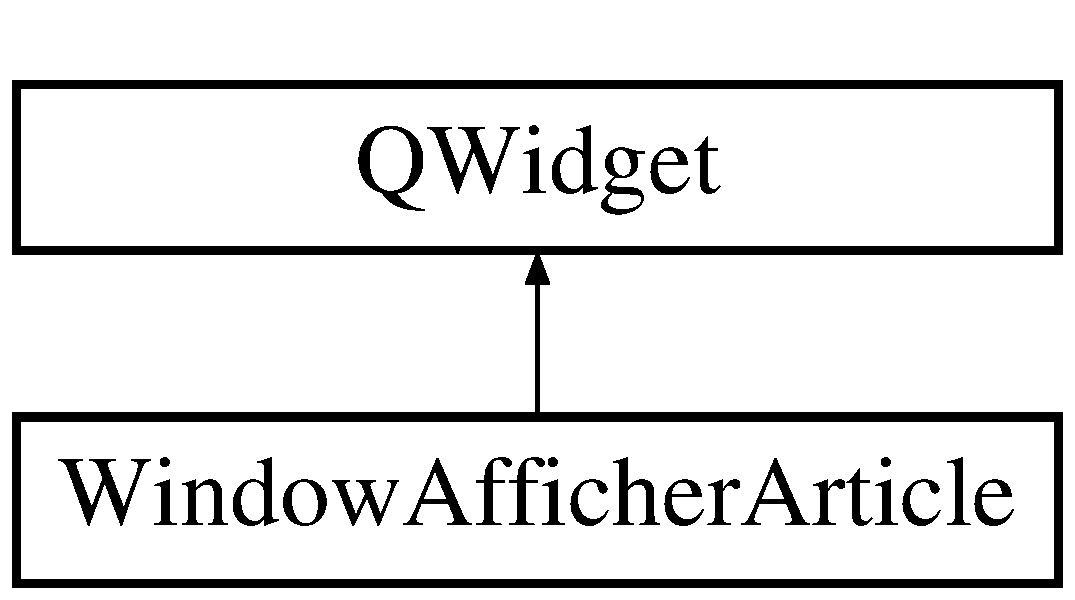
\includegraphics[height=2.000000cm]{class_window_afficher_article}
\end{center}
\end{figure}
\subsection*{Public Member Functions}
\begin{DoxyCompactItemize}
\item 
\hyperlink{class_window_afficher_article_afc3f7e8bf71846a8d1cfa881e4d6e9ca}{Window\+Afficher\+Article} (\hyperlink{class_article}{Article} $\ast$art, Q\+Widget $\ast$parent=0)
\begin{DoxyCompactList}\small\item\em \hyperlink{class_window_afficher_article}{Window\+Afficher\+Article}\+: contructor of the Widget. \end{DoxyCompactList}\item 
Q\+Push\+Button $\ast$ \hyperlink{class_window_afficher_article_a7201792ae876ac84e0a3bf20fd3de313}{get\+Button\+Save} ()
\begin{DoxyCompactList}\small\item\em get\+Button\+Save\+: get the button save \end{DoxyCompactList}\item 
Q\+Line\+Edit $\ast$ \hyperlink{class_window_afficher_article_a2ff36b030fe749ea834d9becb15eedea}{get\+Title} ()
\begin{DoxyCompactList}\small\item\em get\+Title\+: get the line space \end{DoxyCompactList}\item 
Q\+Text\+Edit $\ast$ \hyperlink{class_window_afficher_article_a955158e6061fffdceed9f97dee9486f1}{get\+Text} ()
\begin{DoxyCompactList}\small\item\em get\+Text\+: get the text space \end{DoxyCompactList}\item 
\hyperlink{class_article}{Article} $\ast$ \hyperlink{class_window_afficher_article_acc7b1b026331c6b6fe883ae0c3619b9f}{get\+Article} ()
\begin{DoxyCompactList}\small\item\em get\+Article\+: get the selected article \end{DoxyCompactList}\end{DoxyCompactItemize}


\subsection{Detailed Description}
The \hyperlink{class_window_afficher_article}{Window\+Afficher\+Article} class\+: Widget to view and edit article. 

\subsection{Constructor \& Destructor Documentation}
\mbox{\Hypertarget{class_window_afficher_article_afc3f7e8bf71846a8d1cfa881e4d6e9ca}\label{class_window_afficher_article_afc3f7e8bf71846a8d1cfa881e4d6e9ca}} 
\index{Window\+Afficher\+Article@{Window\+Afficher\+Article}!Window\+Afficher\+Article@{Window\+Afficher\+Article}}
\index{Window\+Afficher\+Article@{Window\+Afficher\+Article}!Window\+Afficher\+Article@{Window\+Afficher\+Article}}
\subsubsection{\texorpdfstring{Window\+Afficher\+Article()}{WindowAfficherArticle()}}
{\footnotesize\ttfamily Window\+Afficher\+Article\+::\+Window\+Afficher\+Article (\begin{DoxyParamCaption}\item[{\hyperlink{class_article}{Article} $\ast$}]{art,  }\item[{Q\+Widget $\ast$}]{parent = {\ttfamily 0} }\end{DoxyParamCaption})}



\hyperlink{class_window_afficher_article}{Window\+Afficher\+Article}\+: contructor of the Widget. 


\begin{DoxyParams}{Parameters}
{\em art} & the choosed article to view and edit \\
\hline
{\em parent} & parent Widget \\
\hline
\end{DoxyParams}


\subsection{Member Function Documentation}
\mbox{\Hypertarget{class_window_afficher_article_acc7b1b026331c6b6fe883ae0c3619b9f}\label{class_window_afficher_article_acc7b1b026331c6b6fe883ae0c3619b9f}} 
\index{Window\+Afficher\+Article@{Window\+Afficher\+Article}!get\+Article@{get\+Article}}
\index{get\+Article@{get\+Article}!Window\+Afficher\+Article@{Window\+Afficher\+Article}}
\subsubsection{\texorpdfstring{get\+Article()}{getArticle()}}
{\footnotesize\ttfamily \hyperlink{class_article}{Article}$\ast$ Window\+Afficher\+Article\+::get\+Article (\begin{DoxyParamCaption}{ }\end{DoxyParamCaption})\hspace{0.3cm}{\ttfamily [inline]}}



get\+Article\+: get the selected article 

\begin{DoxyReturn}{Returns}
pointer to the selected article 
\end{DoxyReturn}
\mbox{\Hypertarget{class_window_afficher_article_a7201792ae876ac84e0a3bf20fd3de313}\label{class_window_afficher_article_a7201792ae876ac84e0a3bf20fd3de313}} 
\index{Window\+Afficher\+Article@{Window\+Afficher\+Article}!get\+Button\+Save@{get\+Button\+Save}}
\index{get\+Button\+Save@{get\+Button\+Save}!Window\+Afficher\+Article@{Window\+Afficher\+Article}}
\subsubsection{\texorpdfstring{get\+Button\+Save()}{getButtonSave()}}
{\footnotesize\ttfamily Q\+Push\+Button$\ast$ Window\+Afficher\+Article\+::get\+Button\+Save (\begin{DoxyParamCaption}{ }\end{DoxyParamCaption})\hspace{0.3cm}{\ttfamily [inline]}}



get\+Button\+Save\+: get the button save 

\begin{DoxyReturn}{Returns}
pointer to the button save 
\end{DoxyReturn}
\mbox{\Hypertarget{class_window_afficher_article_a955158e6061fffdceed9f97dee9486f1}\label{class_window_afficher_article_a955158e6061fffdceed9f97dee9486f1}} 
\index{Window\+Afficher\+Article@{Window\+Afficher\+Article}!get\+Text@{get\+Text}}
\index{get\+Text@{get\+Text}!Window\+Afficher\+Article@{Window\+Afficher\+Article}}
\subsubsection{\texorpdfstring{get\+Text()}{getText()}}
{\footnotesize\ttfamily Q\+Text\+Edit$\ast$ Window\+Afficher\+Article\+::get\+Text (\begin{DoxyParamCaption}{ }\end{DoxyParamCaption})\hspace{0.3cm}{\ttfamily [inline]}}



get\+Text\+: get the text space 

\begin{DoxyReturn}{Returns}
pointer to the text space 
\end{DoxyReturn}
\mbox{\Hypertarget{class_window_afficher_article_a2ff36b030fe749ea834d9becb15eedea}\label{class_window_afficher_article_a2ff36b030fe749ea834d9becb15eedea}} 
\index{Window\+Afficher\+Article@{Window\+Afficher\+Article}!get\+Title@{get\+Title}}
\index{get\+Title@{get\+Title}!Window\+Afficher\+Article@{Window\+Afficher\+Article}}
\subsubsection{\texorpdfstring{get\+Title()}{getTitle()}}
{\footnotesize\ttfamily Q\+Line\+Edit$\ast$ Window\+Afficher\+Article\+::get\+Title (\begin{DoxyParamCaption}{ }\end{DoxyParamCaption})\hspace{0.3cm}{\ttfamily [inline]}}



get\+Title\+: get the line space 

\begin{DoxyReturn}{Returns}
pointer to the line space 
\end{DoxyReturn}


The documentation for this class was generated from the following files\+:\begin{DoxyCompactItemize}
\item 
\hyperlink{wafficherarticle_8h}{wafficherarticle.\+h}\item 
wafficherarticle.\+cpp\end{DoxyCompactItemize}

\hypertarget{class_window_afficher_audio}{}\section{Window\+Afficher\+Audio Class Reference}
\label{class_window_afficher_audio}\index{Window\+Afficher\+Audio@{Window\+Afficher\+Audio}}


Définit la classe \hyperlink{class_window_afficher_audio}{Window\+Afficher\+Audio} \+: Emplacement pour afficher un audio.  




{\ttfamily \#include $<$hafficheraudio.\+h$>$}

Inheritance diagram for Window\+Afficher\+Audio\+:\begin{figure}[H]
\begin{center}
\leavevmode
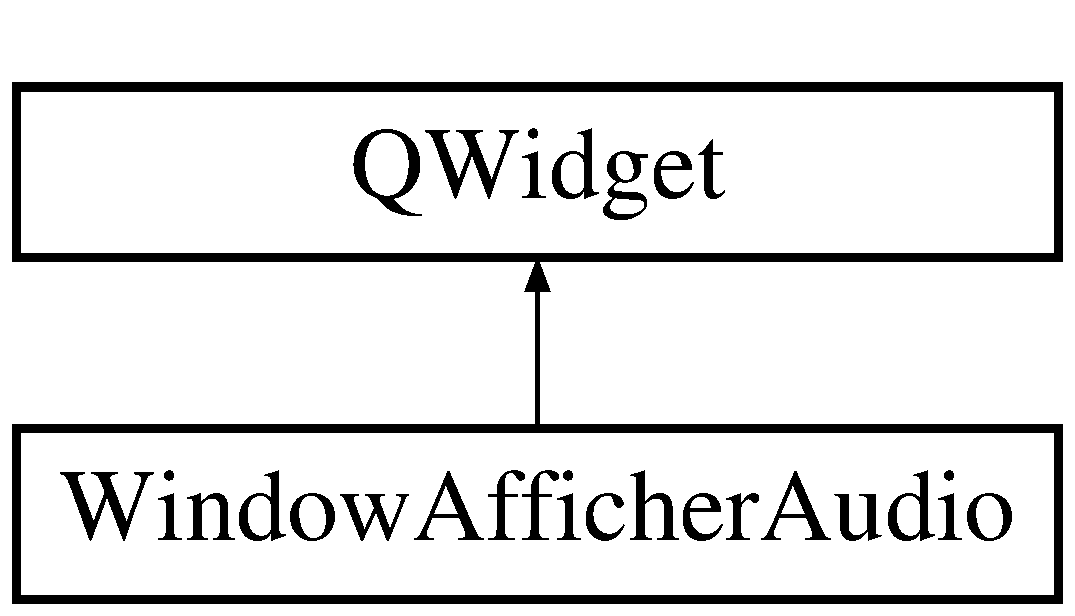
\includegraphics[height=2.000000cm]{class_window_afficher_audio}
\end{center}
\end{figure}
\subsection*{Public Member Functions}
\begin{DoxyCompactItemize}
\item 
\mbox{\Hypertarget{class_window_afficher_audio_a95cd6d56b939154f985c7871b2762533}\label{class_window_afficher_audio_a95cd6d56b939154f985c7871b2762533}} 
{\bfseries Window\+Afficher\+Audio} (\hyperlink{classaudio}{audio} $\ast$au, Q\+Widget $\ast$parent=0)
\item 
\mbox{\Hypertarget{class_window_afficher_audio_aea896e4f759330de7d28e7c244333a0c}\label{class_window_afficher_audio_aea896e4f759330de7d28e7c244333a0c}} 
Q\+Push\+Button $\ast$ {\bfseries get\+Button\+Save} ()
\item 
\mbox{\Hypertarget{class_window_afficher_audio_a580ed7bcb6fff41ce8d44d247d6bfe55}\label{class_window_afficher_audio_a580ed7bcb6fff41ce8d44d247d6bfe55}} 
Q\+Line\+Edit $\ast$ {\bfseries get\+Title} ()
\item 
\mbox{\Hypertarget{class_window_afficher_audio_a04ed86b67f5ca3fb98a052d3201942ab}\label{class_window_afficher_audio_a04ed86b67f5ca3fb98a052d3201942ab}} 
Q\+Text\+Edit $\ast$ {\bfseries get\+Desc} ()
\item 
\mbox{\Hypertarget{class_window_afficher_audio_abbfcec61167e06a68e7d9d2109c5c1fd}\label{class_window_afficher_audio_abbfcec61167e06a68e7d9d2109c5c1fd}} 
Q\+Line\+Edit $\ast$ {\bfseries get\+Chemin} ()
\item 
\mbox{\Hypertarget{class_window_afficher_audio_ae0ff73dae1ca9c4c5ab644a75cb8e100}\label{class_window_afficher_audio_ae0ff73dae1ca9c4c5ab644a75cb8e100}} 
Q\+Line\+Edit $\ast$ {\bfseries get\+Chemin\+Audio} ()
\item 
\mbox{\Hypertarget{class_window_afficher_audio_a082597915a6d0d5fca04c288678725a1}\label{class_window_afficher_audio_a082597915a6d0d5fca04c288678725a1}} 
\hyperlink{classaudio}{audio} $\ast$ {\bfseries get\+Audio} ()
\end{DoxyCompactItemize}


\subsection{Detailed Description}
Définit la classe \hyperlink{class_window_afficher_audio}{Window\+Afficher\+Audio} \+: Emplacement pour afficher un audio. 

Hérite de Q\+Widget audio \+: \hyperlink{class_note}{Note} audio titre\+\_\+text\+: Formulaire titre de la audio desc\+\_\+text\+: Formulaire description de la audio image\+\_\+text\+: Formulaire image de la audio audio\+\_\+text\+: Formulaire audio de la audio valider \+: Bouton valider annuler \+: Bouton annuler 

The documentation for this class was generated from the following files\+:\begin{DoxyCompactItemize}
\item 
\hyperlink{hafficheraudio_8h}{hafficheraudio.\+h}\item 
hafficheraudio.\+cpp\end{DoxyCompactItemize}

\hypertarget{class_window_afficher_couple}{}\section{Window\+Afficher\+Couple Class Reference}
\label{class_window_afficher_couple}\index{Window\+Afficher\+Couple@{Window\+Afficher\+Couple}}


The \hyperlink{class_window_afficher_couple}{Window\+Afficher\+Couple} class\+: the Widget to view all couplees of a relation.  




{\ttfamily \#include $<$waffichercouple.\+h$>$}

Inheritance diagram for Window\+Afficher\+Couple\+:\begin{figure}[H]
\begin{center}
\leavevmode
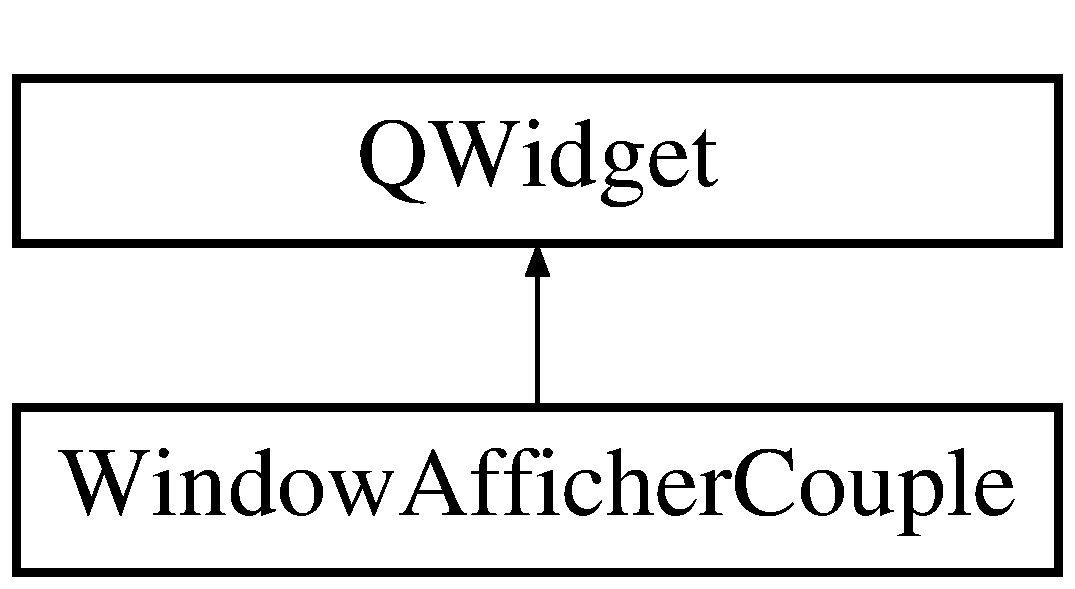
\includegraphics[height=2.000000cm]{class_window_afficher_couple}
\end{center}
\end{figure}
\subsection*{Public Member Functions}
\begin{DoxyCompactItemize}
\item 
\hyperlink{class_window_afficher_couple_a6f57f30e30be963212ea7a355f460c30}{Window\+Afficher\+Couple} (Q\+String \&relation\+\_\+name, Q\+Widget $\ast$parent=0)
\begin{DoxyCompactList}\small\item\em \hyperlink{class_window_afficher_couple}{Window\+Afficher\+Couple}\+: constructor of the Widget. \end{DoxyCompactList}\item 
Q\+Push\+Button $\ast$ \hyperlink{class_window_afficher_couple_af6825c2bdd3c0612409d517f229a5e60}{get\+Button\+Create\+Version} ()
\begin{DoxyCompactList}\small\item\em get\+Button\+Create\+Version\+: get the button to create couple \end{DoxyCompactList}\end{DoxyCompactItemize}


\subsection{Detailed Description}
The \hyperlink{class_window_afficher_couple}{Window\+Afficher\+Couple} class\+: the Widget to view all couplees of a relation. 

\subsection{Constructor \& Destructor Documentation}
\mbox{\Hypertarget{class_window_afficher_couple_a6f57f30e30be963212ea7a355f460c30}\label{class_window_afficher_couple_a6f57f30e30be963212ea7a355f460c30}} 
\index{Window\+Afficher\+Couple@{Window\+Afficher\+Couple}!Window\+Afficher\+Couple@{Window\+Afficher\+Couple}}
\index{Window\+Afficher\+Couple@{Window\+Afficher\+Couple}!Window\+Afficher\+Couple@{Window\+Afficher\+Couple}}
\subsubsection{\texorpdfstring{Window\+Afficher\+Couple()}{WindowAfficherCouple()}}
{\footnotesize\ttfamily Window\+Afficher\+Couple\+::\+Window\+Afficher\+Couple (\begin{DoxyParamCaption}\item[{Q\+String \&}]{relation\+\_\+name,  }\item[{Q\+Widget $\ast$}]{parent = {\ttfamily 0} }\end{DoxyParamCaption})}



\hyperlink{class_window_afficher_couple}{Window\+Afficher\+Couple}\+: constructor of the Widget. 


\begin{DoxyParams}{Parameters}
{\em relation\+\_\+name} & the name of choosed relation \\
\hline
{\em parent} & parent Widget \\
\hline
\end{DoxyParams}


\subsection{Member Function Documentation}
\mbox{\Hypertarget{class_window_afficher_couple_af6825c2bdd3c0612409d517f229a5e60}\label{class_window_afficher_couple_af6825c2bdd3c0612409d517f229a5e60}} 
\index{Window\+Afficher\+Couple@{Window\+Afficher\+Couple}!get\+Button\+Create\+Version@{get\+Button\+Create\+Version}}
\index{get\+Button\+Create\+Version@{get\+Button\+Create\+Version}!Window\+Afficher\+Couple@{Window\+Afficher\+Couple}}
\subsubsection{\texorpdfstring{get\+Button\+Create\+Version()}{getButtonCreateVersion()}}
{\footnotesize\ttfamily Q\+Push\+Button$\ast$ Window\+Afficher\+Couple\+::get\+Button\+Create\+Version (\begin{DoxyParamCaption}{ }\end{DoxyParamCaption})\hspace{0.3cm}{\ttfamily [inline]}}



get\+Button\+Create\+Version\+: get the button to create couple 

\begin{DoxyReturn}{Returns}

\end{DoxyReturn}


The documentation for this class was generated from the following files\+:\begin{DoxyCompactItemize}
\item 
\hyperlink{waffichercouple_8h}{waffichercouple.\+h}\item 
waffichercouple.\+cpp\end{DoxyCompactItemize}

\hypertarget{class_window_afficher_image}{}\section{Window\+Afficher\+Image Class Reference}
\label{class_window_afficher_image}\index{Window\+Afficher\+Image@{Window\+Afficher\+Image}}


The Window\+Afficher\+Imag class\+: Widget to view and edit image.  




{\ttfamily \#include $<$wafficherimage.\+h$>$}

Inheritance diagram for Window\+Afficher\+Image\+:\begin{figure}[H]
\begin{center}
\leavevmode
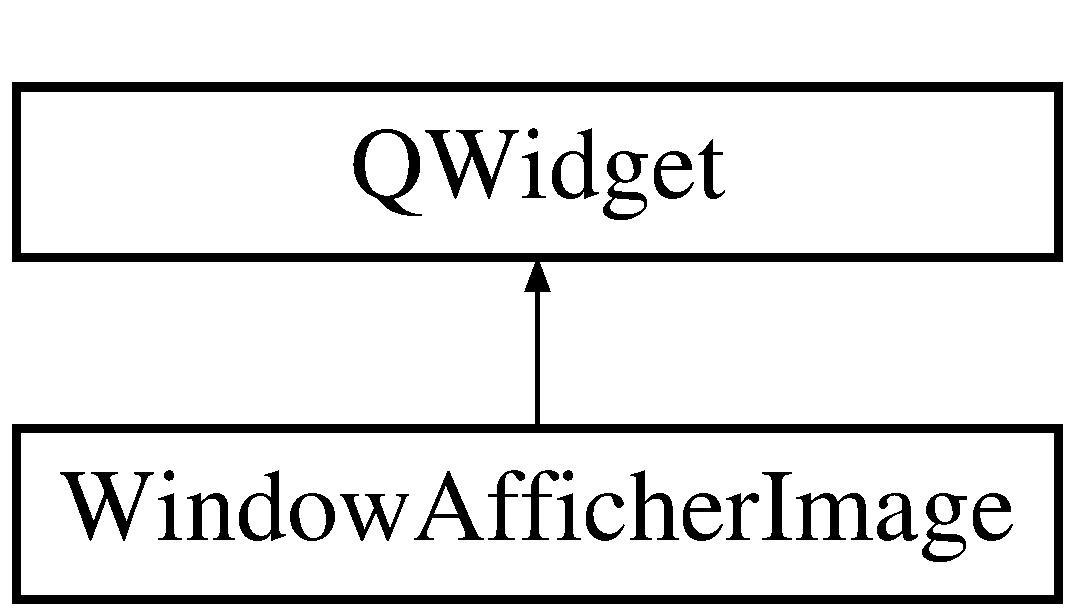
\includegraphics[height=2.000000cm]{class_window_afficher_image}
\end{center}
\end{figure}
\subsection*{Public Member Functions}
\begin{DoxyCompactItemize}
\item 
\hyperlink{class_window_afficher_image_a98a5ee55c190ac82b232248fb1ebde16}{Window\+Afficher\+Image} (\hyperlink{classimage}{image} $\ast$im, Q\+Widget $\ast$parent=0)
\begin{DoxyCompactList}\small\item\em \hyperlink{class_window_afficher_image}{Window\+Afficher\+Image}\+: constructor of the Widget. \end{DoxyCompactList}\item 
Q\+Push\+Button $\ast$ \hyperlink{class_window_afficher_image_ab4d02c68e2c3ae753e7547b114e5bbb3}{get\+Button\+Save} ()
\begin{DoxyCompactList}\small\item\em get\+Button\+Save\+: get the button save \end{DoxyCompactList}\item 
Q\+Line\+Edit $\ast$ \hyperlink{class_window_afficher_image_a2af473bca8e2be4e6aaadaa92b7da192}{get\+Title} ()
\begin{DoxyCompactList}\small\item\em get\+Title\+: get the line space \end{DoxyCompactList}\item 
Q\+Text\+Edit $\ast$ \hyperlink{class_window_afficher_image_a0abeb04216548502d7026bad0c00d0f4}{get\+Desc} ()
\begin{DoxyCompactList}\small\item\em get\+Desc\+: get the text space \end{DoxyCompactList}\item 
Q\+Line\+Edit $\ast$ \hyperlink{class_window_afficher_image_a59e27e3dbd1f2bc4a0d9fe99a20025fb}{get\+Chemin} ()
\begin{DoxyCompactList}\small\item\em get\+Chemin\+: get to the line space directory \end{DoxyCompactList}\item 
\hyperlink{classimage}{image} $\ast$ \hyperlink{class_window_afficher_image_ac8a0d10bb80e99fda8ca7eaf77b072ea}{get\+Image} ()
\begin{DoxyCompactList}\small\item\em get\+Image\+: get the selected image \end{DoxyCompactList}\end{DoxyCompactItemize}


\subsection{Detailed Description}
The Window\+Afficher\+Imag class\+: Widget to view and edit image. 

\subsection{Constructor \& Destructor Documentation}
\mbox{\Hypertarget{class_window_afficher_image_a98a5ee55c190ac82b232248fb1ebde16}\label{class_window_afficher_image_a98a5ee55c190ac82b232248fb1ebde16}} 
\index{Window\+Afficher\+Image@{Window\+Afficher\+Image}!Window\+Afficher\+Image@{Window\+Afficher\+Image}}
\index{Window\+Afficher\+Image@{Window\+Afficher\+Image}!Window\+Afficher\+Image@{Window\+Afficher\+Image}}
\subsubsection{\texorpdfstring{Window\+Afficher\+Image()}{WindowAfficherImage()}}
{\footnotesize\ttfamily Window\+Afficher\+Image\+::\+Window\+Afficher\+Image (\begin{DoxyParamCaption}\item[{\hyperlink{classimage}{image} $\ast$}]{im,  }\item[{Q\+Widget $\ast$}]{parent = {\ttfamily 0} }\end{DoxyParamCaption})}



\hyperlink{class_window_afficher_image}{Window\+Afficher\+Image}\+: constructor of the Widget. 


\begin{DoxyParams}{Parameters}
{\em im} & pointer to selected image \\
\hline
{\em parent} & parent Widget \\
\hline
\end{DoxyParams}


\subsection{Member Function Documentation}
\mbox{\Hypertarget{class_window_afficher_image_ab4d02c68e2c3ae753e7547b114e5bbb3}\label{class_window_afficher_image_ab4d02c68e2c3ae753e7547b114e5bbb3}} 
\index{Window\+Afficher\+Image@{Window\+Afficher\+Image}!get\+Button\+Save@{get\+Button\+Save}}
\index{get\+Button\+Save@{get\+Button\+Save}!Window\+Afficher\+Image@{Window\+Afficher\+Image}}
\subsubsection{\texorpdfstring{get\+Button\+Save()}{getButtonSave()}}
{\footnotesize\ttfamily Q\+Push\+Button$\ast$ Window\+Afficher\+Image\+::get\+Button\+Save (\begin{DoxyParamCaption}{ }\end{DoxyParamCaption})\hspace{0.3cm}{\ttfamily [inline]}}



get\+Button\+Save\+: get the button save 

\begin{DoxyReturn}{Returns}
pointer to the button save 
\end{DoxyReturn}
\mbox{\Hypertarget{class_window_afficher_image_a59e27e3dbd1f2bc4a0d9fe99a20025fb}\label{class_window_afficher_image_a59e27e3dbd1f2bc4a0d9fe99a20025fb}} 
\index{Window\+Afficher\+Image@{Window\+Afficher\+Image}!get\+Chemin@{get\+Chemin}}
\index{get\+Chemin@{get\+Chemin}!Window\+Afficher\+Image@{Window\+Afficher\+Image}}
\subsubsection{\texorpdfstring{get\+Chemin()}{getChemin()}}
{\footnotesize\ttfamily Q\+Line\+Edit$\ast$ Window\+Afficher\+Image\+::get\+Chemin (\begin{DoxyParamCaption}{ }\end{DoxyParamCaption})\hspace{0.3cm}{\ttfamily [inline]}}



get\+Chemin\+: get to the line space directory 

\begin{DoxyReturn}{Returns}
pointer to line space 
\end{DoxyReturn}
\mbox{\Hypertarget{class_window_afficher_image_a0abeb04216548502d7026bad0c00d0f4}\label{class_window_afficher_image_a0abeb04216548502d7026bad0c00d0f4}} 
\index{Window\+Afficher\+Image@{Window\+Afficher\+Image}!get\+Desc@{get\+Desc}}
\index{get\+Desc@{get\+Desc}!Window\+Afficher\+Image@{Window\+Afficher\+Image}}
\subsubsection{\texorpdfstring{get\+Desc()}{getDesc()}}
{\footnotesize\ttfamily Q\+Text\+Edit$\ast$ Window\+Afficher\+Image\+::get\+Desc (\begin{DoxyParamCaption}{ }\end{DoxyParamCaption})\hspace{0.3cm}{\ttfamily [inline]}}



get\+Desc\+: get the text space 

\begin{DoxyReturn}{Returns}
pointer to the text space 
\end{DoxyReturn}
\mbox{\Hypertarget{class_window_afficher_image_ac8a0d10bb80e99fda8ca7eaf77b072ea}\label{class_window_afficher_image_ac8a0d10bb80e99fda8ca7eaf77b072ea}} 
\index{Window\+Afficher\+Image@{Window\+Afficher\+Image}!get\+Image@{get\+Image}}
\index{get\+Image@{get\+Image}!Window\+Afficher\+Image@{Window\+Afficher\+Image}}
\subsubsection{\texorpdfstring{get\+Image()}{getImage()}}
{\footnotesize\ttfamily \hyperlink{classimage}{image}$\ast$ Window\+Afficher\+Image\+::get\+Image (\begin{DoxyParamCaption}{ }\end{DoxyParamCaption})\hspace{0.3cm}{\ttfamily [inline]}}



get\+Image\+: get the selected image 

\begin{DoxyReturn}{Returns}
pointer to the seleted iamge 
\end{DoxyReturn}
\mbox{\Hypertarget{class_window_afficher_image_a2af473bca8e2be4e6aaadaa92b7da192}\label{class_window_afficher_image_a2af473bca8e2be4e6aaadaa92b7da192}} 
\index{Window\+Afficher\+Image@{Window\+Afficher\+Image}!get\+Title@{get\+Title}}
\index{get\+Title@{get\+Title}!Window\+Afficher\+Image@{Window\+Afficher\+Image}}
\subsubsection{\texorpdfstring{get\+Title()}{getTitle()}}
{\footnotesize\ttfamily Q\+Line\+Edit$\ast$ Window\+Afficher\+Image\+::get\+Title (\begin{DoxyParamCaption}{ }\end{DoxyParamCaption})\hspace{0.3cm}{\ttfamily [inline]}}



get\+Title\+: get the line space 

\begin{DoxyReturn}{Returns}
pointer to the line space 
\end{DoxyReturn}


The documentation for this class was generated from the following files\+:\begin{DoxyCompactItemize}
\item 
\hyperlink{wafficherimage_8h}{wafficherimage.\+h}\item 
wafficherimage.\+cpp\end{DoxyCompactItemize}

\hypertarget{class_window_afficher_tache}{}\section{Window\+Afficher\+Tache Class Reference}
\label{class_window_afficher_tache}\index{Window\+Afficher\+Tache@{Window\+Afficher\+Tache}}
Inheritance diagram for Window\+Afficher\+Tache\+:\begin{figure}[H]
\begin{center}
\leavevmode
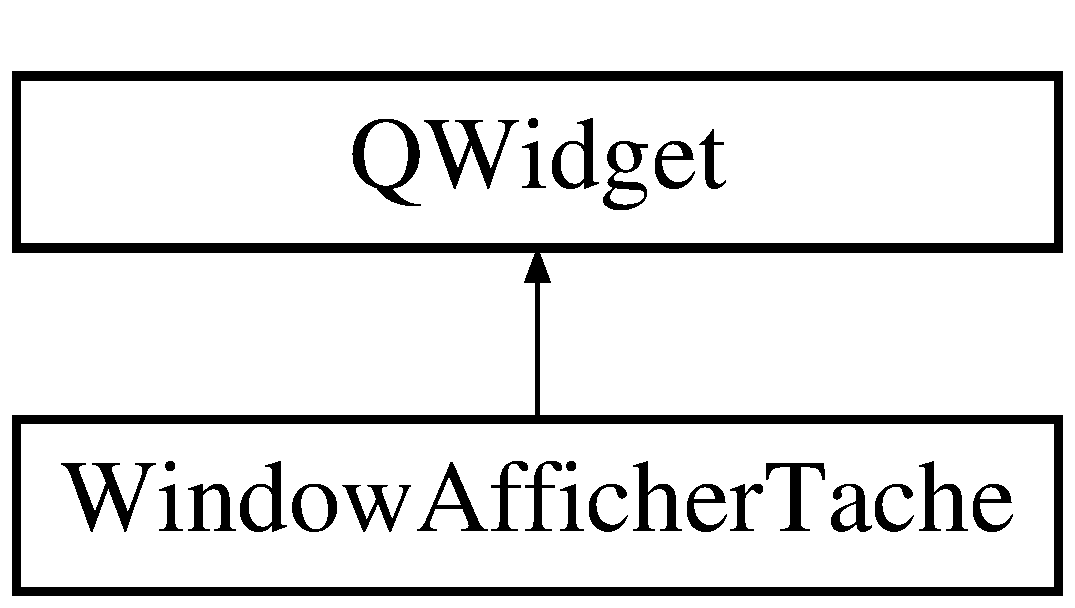
\includegraphics[height=2.000000cm]{class_window_afficher_tache}
\end{center}
\end{figure}
\subsection*{Public Member Functions}
\begin{DoxyCompactItemize}
\item 
\hyperlink{class_window_afficher_tache_a05d3a934243ff05e1120f07c84efd1fc}{Window\+Afficher\+Tache} (\hyperlink{class_tache}{Tache} $\ast$ta, Q\+Widget $\ast$parent=0)
\begin{DoxyCompactList}\small\item\em \hyperlink{class_window_afficher_tache}{Window\+Afficher\+Tache}\+: contructor of the Widget. \end{DoxyCompactList}\item 
Q\+Push\+Button $\ast$ \hyperlink{class_window_afficher_tache_a8a5df0c8f8b2ace2c5f09daa1cbaa7eb}{get\+Button\+Save} ()
\begin{DoxyCompactList}\small\item\em get\+Button\+Save\+: get the button save \end{DoxyCompactList}\item 
Q\+Line\+Edit $\ast$ \hyperlink{class_window_afficher_tache_a65f59931ef68115aad28770e998eabd5}{get\+Title} ()
\begin{DoxyCompactList}\small\item\em get\+Title\+: get the line space of titre \end{DoxyCompactList}\item 
Q\+Text\+Edit $\ast$ \hyperlink{class_window_afficher_tache_a5fe2e2ee086218f44e4223ce5eeae84c}{get\+Text\+Box} ()
\begin{DoxyCompactList}\small\item\em get\+Text\+Box\+: get action text space \end{DoxyCompactList}\item 
Q\+Line\+Edit $\ast$ \hyperlink{class_window_afficher_tache_ae47fad44c28bba49406b648cb452038d}{get\+Statut\+Box} ()
\begin{DoxyCompactList}\small\item\em get\+Title\+: get the line space of status \end{DoxyCompactList}\item 
Q\+Line\+Edit $\ast$ \hyperlink{class_window_afficher_tache_a2a51fbf9e0089f92bc0b96d2ac7f38a6}{get\+Prio\+Box} ()
\begin{DoxyCompactList}\small\item\em get\+Prio\+Box\+: get the line space of priority \end{DoxyCompactList}\item 
Q\+Line\+Edit $\ast$ \hyperlink{class_window_afficher_tache_ac1bfa30c803531cf3119de9dcf2169ee}{get\+Date\+\_\+e\+\_\+\+Day\+Box} ()
\begin{DoxyCompactList}\small\item\em get\+Date\+\_\+e\+\_\+\+Day\+Box\+: get the line space of date\+\_\+e\+\_\+day\+\_\+box \end{DoxyCompactList}\end{DoxyCompactItemize}


\subsection{Constructor \& Destructor Documentation}
\mbox{\Hypertarget{class_window_afficher_tache_a05d3a934243ff05e1120f07c84efd1fc}\label{class_window_afficher_tache_a05d3a934243ff05e1120f07c84efd1fc}} 
\index{Window\+Afficher\+Tache@{Window\+Afficher\+Tache}!Window\+Afficher\+Tache@{Window\+Afficher\+Tache}}
\index{Window\+Afficher\+Tache@{Window\+Afficher\+Tache}!Window\+Afficher\+Tache@{Window\+Afficher\+Tache}}
\subsubsection{\texorpdfstring{Window\+Afficher\+Tache()}{WindowAfficherTache()}}
{\footnotesize\ttfamily Window\+Afficher\+Tache\+::\+Window\+Afficher\+Tache (\begin{DoxyParamCaption}\item[{\hyperlink{class_tache}{Tache} $\ast$}]{ta,  }\item[{Q\+Widget $\ast$}]{parent = {\ttfamily 0} }\end{DoxyParamCaption})}



\hyperlink{class_window_afficher_tache}{Window\+Afficher\+Tache}\+: contructor of the Widget. 


\begin{DoxyParams}{Parameters}
{\em ta} & the choosed tache to view and edit \\
\hline
{\em parent} & parent Widget \\
\hline
\end{DoxyParams}


\subsection{Member Function Documentation}
\mbox{\Hypertarget{class_window_afficher_tache_a8a5df0c8f8b2ace2c5f09daa1cbaa7eb}\label{class_window_afficher_tache_a8a5df0c8f8b2ace2c5f09daa1cbaa7eb}} 
\index{Window\+Afficher\+Tache@{Window\+Afficher\+Tache}!get\+Button\+Save@{get\+Button\+Save}}
\index{get\+Button\+Save@{get\+Button\+Save}!Window\+Afficher\+Tache@{Window\+Afficher\+Tache}}
\subsubsection{\texorpdfstring{get\+Button\+Save()}{getButtonSave()}}
{\footnotesize\ttfamily Q\+Push\+Button$\ast$ Window\+Afficher\+Tache\+::get\+Button\+Save (\begin{DoxyParamCaption}{ }\end{DoxyParamCaption})\hspace{0.3cm}{\ttfamily [inline]}}



get\+Button\+Save\+: get the button save 

\begin{DoxyReturn}{Returns}
pointer to the button save 
\end{DoxyReturn}
\mbox{\Hypertarget{class_window_afficher_tache_ac1bfa30c803531cf3119de9dcf2169ee}\label{class_window_afficher_tache_ac1bfa30c803531cf3119de9dcf2169ee}} 
\index{Window\+Afficher\+Tache@{Window\+Afficher\+Tache}!get\+Date\+\_\+e\+\_\+\+Day\+Box@{get\+Date\+\_\+e\+\_\+\+Day\+Box}}
\index{get\+Date\+\_\+e\+\_\+\+Day\+Box@{get\+Date\+\_\+e\+\_\+\+Day\+Box}!Window\+Afficher\+Tache@{Window\+Afficher\+Tache}}
\subsubsection{\texorpdfstring{get\+Date\+\_\+e\+\_\+\+Day\+Box()}{getDate\_e\_DayBox()}}
{\footnotesize\ttfamily Q\+Line\+Edit$\ast$ Window\+Afficher\+Tache\+::get\+Date\+\_\+e\+\_\+\+Day\+Box (\begin{DoxyParamCaption}{ }\end{DoxyParamCaption})\hspace{0.3cm}{\ttfamily [inline]}}



get\+Date\+\_\+e\+\_\+\+Day\+Box\+: get the line space of date\+\_\+e\+\_\+day\+\_\+box 

\begin{DoxyReturn}{Returns}
pointer to the line space of date\+\_\+e\+\_\+day\+\_\+box 
\end{DoxyReturn}
\mbox{\Hypertarget{class_window_afficher_tache_a2a51fbf9e0089f92bc0b96d2ac7f38a6}\label{class_window_afficher_tache_a2a51fbf9e0089f92bc0b96d2ac7f38a6}} 
\index{Window\+Afficher\+Tache@{Window\+Afficher\+Tache}!get\+Prio\+Box@{get\+Prio\+Box}}
\index{get\+Prio\+Box@{get\+Prio\+Box}!Window\+Afficher\+Tache@{Window\+Afficher\+Tache}}
\subsubsection{\texorpdfstring{get\+Prio\+Box()}{getPrioBox()}}
{\footnotesize\ttfamily Q\+Line\+Edit$\ast$ Window\+Afficher\+Tache\+::get\+Prio\+Box (\begin{DoxyParamCaption}{ }\end{DoxyParamCaption})\hspace{0.3cm}{\ttfamily [inline]}}



get\+Prio\+Box\+: get the line space of priority 

\begin{DoxyReturn}{Returns}
pointer to the line space of priority 
\end{DoxyReturn}
\mbox{\Hypertarget{class_window_afficher_tache_ae47fad44c28bba49406b648cb452038d}\label{class_window_afficher_tache_ae47fad44c28bba49406b648cb452038d}} 
\index{Window\+Afficher\+Tache@{Window\+Afficher\+Tache}!get\+Statut\+Box@{get\+Statut\+Box}}
\index{get\+Statut\+Box@{get\+Statut\+Box}!Window\+Afficher\+Tache@{Window\+Afficher\+Tache}}
\subsubsection{\texorpdfstring{get\+Statut\+Box()}{getStatutBox()}}
{\footnotesize\ttfamily Q\+Line\+Edit$\ast$ Window\+Afficher\+Tache\+::get\+Statut\+Box (\begin{DoxyParamCaption}{ }\end{DoxyParamCaption})\hspace{0.3cm}{\ttfamily [inline]}}



get\+Title\+: get the line space of status 

\begin{DoxyReturn}{Returns}
pointer to the line space of status 
\end{DoxyReturn}
\mbox{\Hypertarget{class_window_afficher_tache_a5fe2e2ee086218f44e4223ce5eeae84c}\label{class_window_afficher_tache_a5fe2e2ee086218f44e4223ce5eeae84c}} 
\index{Window\+Afficher\+Tache@{Window\+Afficher\+Tache}!get\+Text\+Box@{get\+Text\+Box}}
\index{get\+Text\+Box@{get\+Text\+Box}!Window\+Afficher\+Tache@{Window\+Afficher\+Tache}}
\subsubsection{\texorpdfstring{get\+Text\+Box()}{getTextBox()}}
{\footnotesize\ttfamily Q\+Text\+Edit$\ast$ Window\+Afficher\+Tache\+::get\+Text\+Box (\begin{DoxyParamCaption}{ }\end{DoxyParamCaption})\hspace{0.3cm}{\ttfamily [inline]}}



get\+Text\+Box\+: get action text space 

\begin{DoxyReturn}{Returns}
pointer to the text space 
\end{DoxyReturn}
\mbox{\Hypertarget{class_window_afficher_tache_a65f59931ef68115aad28770e998eabd5}\label{class_window_afficher_tache_a65f59931ef68115aad28770e998eabd5}} 
\index{Window\+Afficher\+Tache@{Window\+Afficher\+Tache}!get\+Title@{get\+Title}}
\index{get\+Title@{get\+Title}!Window\+Afficher\+Tache@{Window\+Afficher\+Tache}}
\subsubsection{\texorpdfstring{get\+Title()}{getTitle()}}
{\footnotesize\ttfamily Q\+Line\+Edit$\ast$ Window\+Afficher\+Tache\+::get\+Title (\begin{DoxyParamCaption}{ }\end{DoxyParamCaption})\hspace{0.3cm}{\ttfamily [inline]}}



get\+Title\+: get the line space of titre 

\begin{DoxyReturn}{Returns}
pointer to the line space of titre 
\end{DoxyReturn}


The documentation for this class was generated from the following files\+:\begin{DoxyCompactItemize}
\item 
\hyperlink{waffichertache_8h}{waffichertache.\+h}\item 
waffichertache.\+cpp\end{DoxyCompactItemize}

\hypertarget{class_window_afficher_video}{}\section{Window\+Afficher\+Video Class Reference}
\label{class_window_afficher_video}\index{Window\+Afficher\+Video@{Window\+Afficher\+Video}}


Définit la classe \hyperlink{class_window_afficher_video}{Window\+Afficher\+Video} \+: Emplacement pour afficher un video.  




{\ttfamily \#include $<$haffichervideo.\+h$>$}

Inheritance diagram for Window\+Afficher\+Video\+:\begin{figure}[H]
\begin{center}
\leavevmode
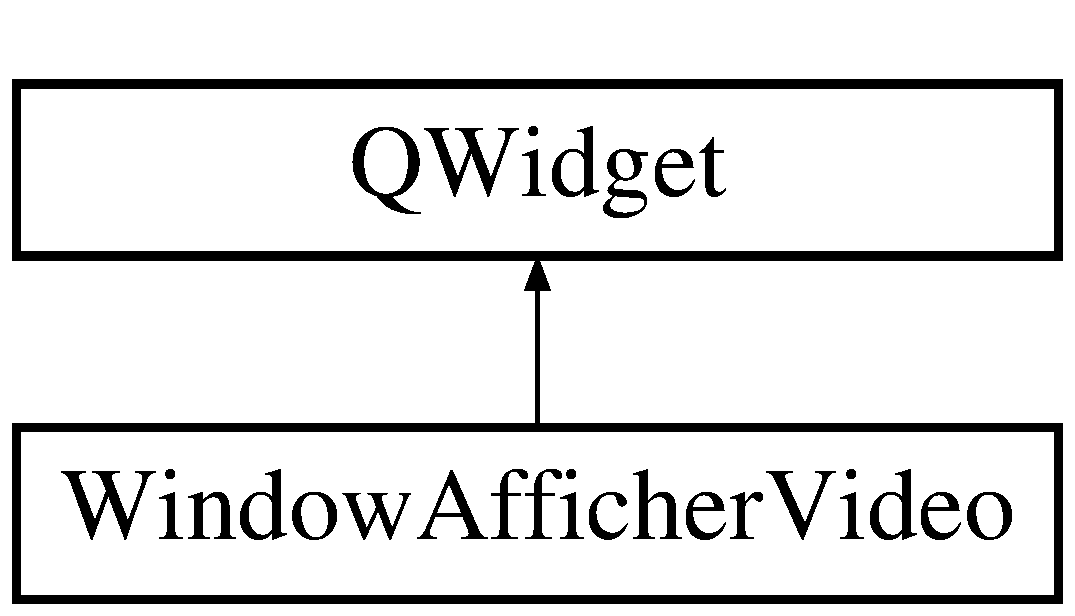
\includegraphics[height=2.000000cm]{class_window_afficher_video}
\end{center}
\end{figure}
\subsection*{Public Member Functions}
\begin{DoxyCompactItemize}
\item 
\mbox{\Hypertarget{class_window_afficher_video_aedcddf13d2b603cb62243fc03d9baed7}\label{class_window_afficher_video_aedcddf13d2b603cb62243fc03d9baed7}} 
{\bfseries Window\+Afficher\+Video} (\hyperlink{classvideo}{video} $\ast$vi, Q\+Widget $\ast$parent=0)
\item 
\mbox{\Hypertarget{class_window_afficher_video_a0f6a04c1f77238072715c18d154abc55}\label{class_window_afficher_video_a0f6a04c1f77238072715c18d154abc55}} 
Q\+Push\+Button $\ast$ {\bfseries get\+Button\+Save} ()
\item 
\mbox{\Hypertarget{class_window_afficher_video_a6a249cb70e3cb731e904ac32c402a132}\label{class_window_afficher_video_a6a249cb70e3cb731e904ac32c402a132}} 
Q\+Line\+Edit $\ast$ {\bfseries get\+Title} ()
\item 
\mbox{\Hypertarget{class_window_afficher_video_a6e331106156efe2aa20f2e2a3ef50288}\label{class_window_afficher_video_a6e331106156efe2aa20f2e2a3ef50288}} 
Q\+Text\+Edit $\ast$ {\bfseries get\+Desc} ()
\item 
\mbox{\Hypertarget{class_window_afficher_video_a04f10264a64ea1f9b53ffc251f3db367}\label{class_window_afficher_video_a04f10264a64ea1f9b53ffc251f3db367}} 
Q\+Line\+Edit $\ast$ {\bfseries get\+Chemin} ()
\item 
\mbox{\Hypertarget{class_window_afficher_video_ab97619282397705914ab85e61320e69d}\label{class_window_afficher_video_ab97619282397705914ab85e61320e69d}} 
Q\+Line\+Edit $\ast$ {\bfseries get\+Chemin\+Video} ()
\item 
\mbox{\Hypertarget{class_window_afficher_video_a047e278dbc118e01521c1238a6130358}\label{class_window_afficher_video_a047e278dbc118e01521c1238a6130358}} 
\hyperlink{classvideo}{video} $\ast$ {\bfseries get\+Video} ()
\end{DoxyCompactItemize}


\subsection{Detailed Description}
Définit la classe \hyperlink{class_window_afficher_video}{Window\+Afficher\+Video} \+: Emplacement pour afficher un video. 

Hérite de Q\+Widget video \+: \hyperlink{class_note}{Note} video titre\+\_\+text\+: Formulaire titre de la video desc\+\_\+text\+: Formulaire description de la video image\+\_\+text\+: Formulaire image de la video video\+\_\+text\+: Formulaire video de la video valider \+: Bouton valider annuler \+: Bouton annuler 

The documentation for this class was generated from the following files\+:\begin{DoxyCompactItemize}
\item 
\hyperlink{haffichervideo_8h}{haffichervideo.\+h}\item 
waffichervideo.\+cpp\end{DoxyCompactItemize}

\hypertarget{class_window_creer_article}{}\section{Window\+Creer\+Article Class Reference}
\label{class_window_creer_article}\index{Window\+Creer\+Article@{Window\+Creer\+Article}}


The \hyperlink{class_window_creer_article}{Window\+Creer\+Article} class\+: Widget to create new article.  




{\ttfamily \#include $<$wcreerarticle.\+h$>$}

Inheritance diagram for Window\+Creer\+Article\+:\begin{figure}[H]
\begin{center}
\leavevmode
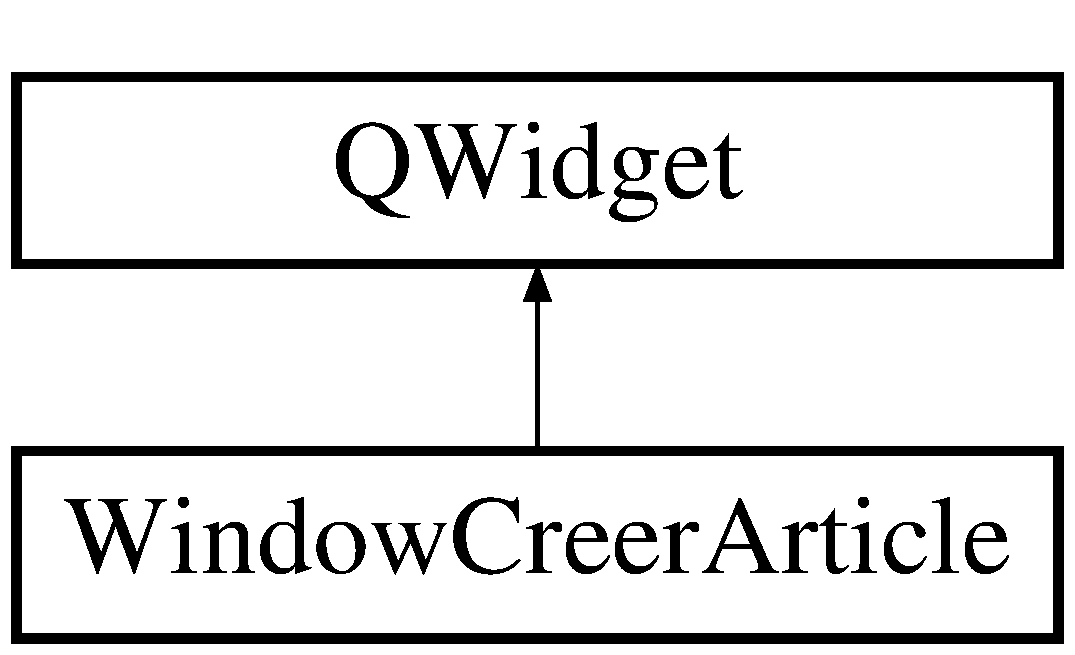
\includegraphics[height=2.000000cm]{class_window_creer_article}
\end{center}
\end{figure}
\subsection*{Public Slots}
\begin{DoxyCompactItemize}
\item 
\mbox{\Hypertarget{class_window_creer_article_a084c06c7c51d4383018ff3d43a081b80}\label{class_window_creer_article_a084c06c7c51d4383018ff3d43a081b80}} 
void \hyperlink{class_window_creer_article_a084c06c7c51d4383018ff3d43a081b80}{create} ()
\begin{DoxyCompactList}\small\item\em create\+: create a new article \end{DoxyCompactList}\end{DoxyCompactItemize}
\subsection*{Public Member Functions}
\begin{DoxyCompactItemize}
\item 
\hyperlink{class_window_creer_article_a671c555bd8bbfbe756c083564487d060}{Window\+Creer\+Article} (Q\+String \&ident, Q\+String \&titre, Q\+Widget $\ast$parent=0)
\begin{DoxyCompactList}\small\item\em \hyperlink{class_window_creer_article}{Window\+Creer\+Article}\+: contructor of the Widget. \end{DoxyCompactList}\item 
Q\+Push\+Button $\ast$ \hyperlink{class_window_creer_article_a9ad8fafa868025bf32085515d5c32f10}{get\+Button\+Create} ()
\begin{DoxyCompactList}\small\item\em get\+Button\+Create\+: get the button create \end{DoxyCompactList}\item 
Q\+Text\+Edit $\ast$ \hyperlink{class_window_creer_article_a3360676f4cc24185a3af311353c3c356}{get\+Text\+Box} ()
\begin{DoxyCompactList}\small\item\em get\+Text\+Box\+: get the line space \end{DoxyCompactList}\end{DoxyCompactItemize}


\subsection{Detailed Description}
The \hyperlink{class_window_creer_article}{Window\+Creer\+Article} class\+: Widget to create new article. 

\subsection{Constructor \& Destructor Documentation}
\mbox{\Hypertarget{class_window_creer_article_a671c555bd8bbfbe756c083564487d060}\label{class_window_creer_article_a671c555bd8bbfbe756c083564487d060}} 
\index{Window\+Creer\+Article@{Window\+Creer\+Article}!Window\+Creer\+Article@{Window\+Creer\+Article}}
\index{Window\+Creer\+Article@{Window\+Creer\+Article}!Window\+Creer\+Article@{Window\+Creer\+Article}}
\subsubsection{\texorpdfstring{Window\+Creer\+Article()}{WindowCreerArticle()}}
{\footnotesize\ttfamily Window\+Creer\+Article\+::\+Window\+Creer\+Article (\begin{DoxyParamCaption}\item[{Q\+String \&}]{ident,  }\item[{Q\+String \&}]{titre,  }\item[{Q\+Widget $\ast$}]{parent = {\ttfamily 0} }\end{DoxyParamCaption})}



\hyperlink{class_window_creer_article}{Window\+Creer\+Article}\+: contructor of the Widget. 


\begin{DoxyParams}{Parameters}
{\em ident} & the identifiant of the new article \\
\hline
{\em parent} & parent Widget \\
\hline
\end{DoxyParams}


\subsection{Member Function Documentation}
\mbox{\Hypertarget{class_window_creer_article_a9ad8fafa868025bf32085515d5c32f10}\label{class_window_creer_article_a9ad8fafa868025bf32085515d5c32f10}} 
\index{Window\+Creer\+Article@{Window\+Creer\+Article}!get\+Button\+Create@{get\+Button\+Create}}
\index{get\+Button\+Create@{get\+Button\+Create}!Window\+Creer\+Article@{Window\+Creer\+Article}}
\subsubsection{\texorpdfstring{get\+Button\+Create()}{getButtonCreate()}}
{\footnotesize\ttfamily Q\+Push\+Button$\ast$ Window\+Creer\+Article\+::get\+Button\+Create (\begin{DoxyParamCaption}{ }\end{DoxyParamCaption})\hspace{0.3cm}{\ttfamily [inline]}}



get\+Button\+Create\+: get the button create 

\begin{DoxyReturn}{Returns}
pointer to the button create 
\end{DoxyReturn}
\mbox{\Hypertarget{class_window_creer_article_a3360676f4cc24185a3af311353c3c356}\label{class_window_creer_article_a3360676f4cc24185a3af311353c3c356}} 
\index{Window\+Creer\+Article@{Window\+Creer\+Article}!get\+Text\+Box@{get\+Text\+Box}}
\index{get\+Text\+Box@{get\+Text\+Box}!Window\+Creer\+Article@{Window\+Creer\+Article}}
\subsubsection{\texorpdfstring{get\+Text\+Box()}{getTextBox()}}
{\footnotesize\ttfamily Q\+Text\+Edit$\ast$ Window\+Creer\+Article\+::get\+Text\+Box (\begin{DoxyParamCaption}{ }\end{DoxyParamCaption})\hspace{0.3cm}{\ttfamily [inline]}}



get\+Text\+Box\+: get the line space 

\begin{DoxyReturn}{Returns}
pointer to the line space 
\end{DoxyReturn}


The documentation for this class was generated from the following files\+:\begin{DoxyCompactItemize}
\item 
\hyperlink{wcreerarticle_8h}{wcreerarticle.\+h}\item 
wcreerarticle.\+cpp\end{DoxyCompactItemize}

\hypertarget{class_window_creer_audio}{}\section{Window\+Creer\+Audio Class Reference}
\label{class_window_creer_audio}\index{Window\+Creer\+Audio@{Window\+Creer\+Audio}}


The \hyperlink{class_window_creer_audio}{Window\+Creer\+Audio} class\+: Widget to create new audio.  




{\ttfamily \#include $<$wcreeraudio.\+h$>$}

Inheritance diagram for Window\+Creer\+Audio\+:\begin{figure}[H]
\begin{center}
\leavevmode
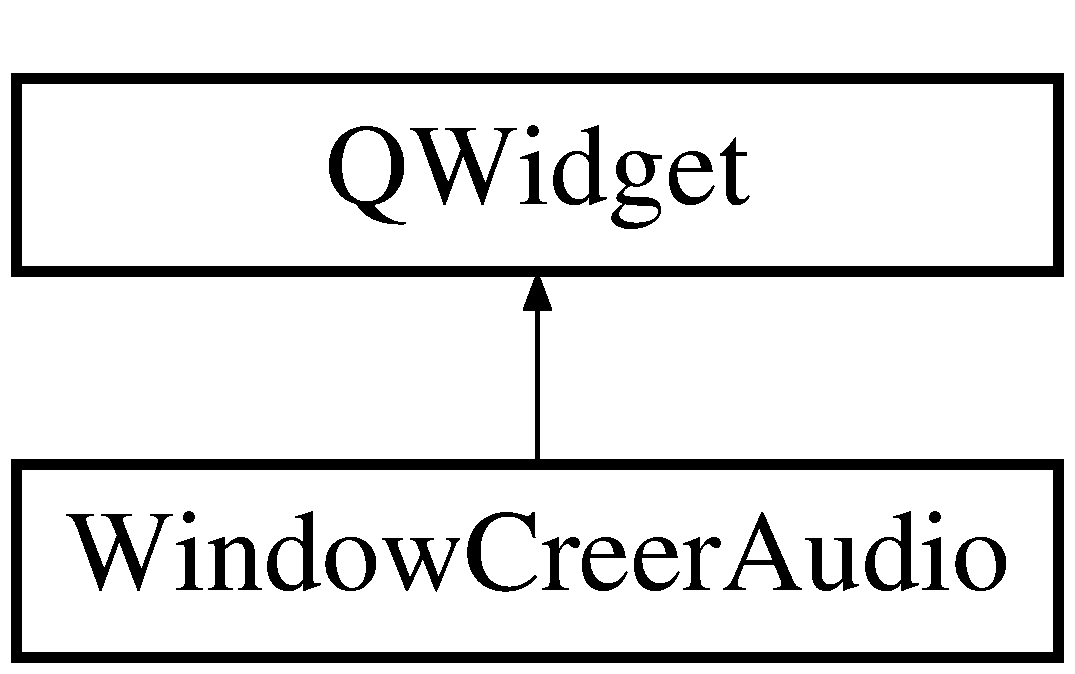
\includegraphics[height=2.000000cm]{class_window_creer_audio}
\end{center}
\end{figure}
\subsection*{Public Slots}
\begin{DoxyCompactItemize}
\item 
\mbox{\Hypertarget{class_window_creer_audio_aaf356899dc6e9892ce190d8dde9dfe33}\label{class_window_creer_audio_aaf356899dc6e9892ce190d8dde9dfe33}} 
void \hyperlink{class_window_creer_audio_aaf356899dc6e9892ce190d8dde9dfe33}{create} ()
\begin{DoxyCompactList}\small\item\em create\+: create a new audio \end{DoxyCompactList}\end{DoxyCompactItemize}
\subsection*{Public Member Functions}
\begin{DoxyCompactItemize}
\item 
\hyperlink{class_window_creer_audio_a48d3b4969c255f0565409a6dcf80014d}{Window\+Creer\+Audio} (Q\+String \&ident, Q\+String \&titre, Q\+Widget $\ast$parent=0)
\begin{DoxyCompactList}\small\item\em \hyperlink{class_window_creer_audio}{Window\+Creer\+Audio}\+: contructor of the Widget. \end{DoxyCompactList}\item 
Q\+Push\+Button $\ast$ \hyperlink{class_window_creer_audio_add4e3e8a08180957f799e465b34efc7d}{get\+Button\+Create} ()
\begin{DoxyCompactList}\small\item\em get\+Button\+Create\+: get the button create \end{DoxyCompactList}\item 
Q\+Text\+Edit $\ast$ \hyperlink{class_window_creer_audio_af644ad3d65f69e77c4d228773b010155}{get\+Desc\+Box} ()
\begin{DoxyCompactList}\small\item\em get\+Desc\+Box\+: get the line space \end{DoxyCompactList}\item 
Q\+Line\+Edit $\ast$ \hyperlink{class_window_creer_audio_a8a6ff8cfc8cfee7a68ba522af12fcb4e}{get\+Image\+Box} ()
\begin{DoxyCompactList}\small\item\em get\+Image\+Box\+: get the line space \end{DoxyCompactList}\item 
Q\+Line\+Edit $\ast$ \hyperlink{class_window_creer_audio_a906b5837d7df59111a0db173e0f48b3b}{get\+Audio\+Box} ()
\begin{DoxyCompactList}\small\item\em get\+Audio\+Box\+: get the line space \end{DoxyCompactList}\end{DoxyCompactItemize}


\subsection{Detailed Description}
The \hyperlink{class_window_creer_audio}{Window\+Creer\+Audio} class\+: Widget to create new audio. 

\subsection{Constructor \& Destructor Documentation}
\mbox{\Hypertarget{class_window_creer_audio_a48d3b4969c255f0565409a6dcf80014d}\label{class_window_creer_audio_a48d3b4969c255f0565409a6dcf80014d}} 
\index{Window\+Creer\+Audio@{Window\+Creer\+Audio}!Window\+Creer\+Audio@{Window\+Creer\+Audio}}
\index{Window\+Creer\+Audio@{Window\+Creer\+Audio}!Window\+Creer\+Audio@{Window\+Creer\+Audio}}
\subsubsection{\texorpdfstring{Window\+Creer\+Audio()}{WindowCreerAudio()}}
{\footnotesize\ttfamily Window\+Creer\+Audio\+::\+Window\+Creer\+Audio (\begin{DoxyParamCaption}\item[{Q\+String \&}]{ident,  }\item[{Q\+String \&}]{titre,  }\item[{Q\+Widget $\ast$}]{parent = {\ttfamily 0} }\end{DoxyParamCaption})}



\hyperlink{class_window_creer_audio}{Window\+Creer\+Audio}\+: contructor of the Widget. 


\begin{DoxyParams}{Parameters}
{\em ident} & the identifiant of the new audio \\
\hline
{\em parent} & parent Widget \\
\hline
\end{DoxyParams}


\subsection{Member Function Documentation}
\mbox{\Hypertarget{class_window_creer_audio_a906b5837d7df59111a0db173e0f48b3b}\label{class_window_creer_audio_a906b5837d7df59111a0db173e0f48b3b}} 
\index{Window\+Creer\+Audio@{Window\+Creer\+Audio}!get\+Audio\+Box@{get\+Audio\+Box}}
\index{get\+Audio\+Box@{get\+Audio\+Box}!Window\+Creer\+Audio@{Window\+Creer\+Audio}}
\subsubsection{\texorpdfstring{get\+Audio\+Box()}{getAudioBox()}}
{\footnotesize\ttfamily Q\+Line\+Edit$\ast$ Window\+Creer\+Audio\+::get\+Audio\+Box (\begin{DoxyParamCaption}{ }\end{DoxyParamCaption})\hspace{0.3cm}{\ttfamily [inline]}}



get\+Audio\+Box\+: get the line space 

\begin{DoxyReturn}{Returns}
pointer to the line space 
\end{DoxyReturn}
\mbox{\Hypertarget{class_window_creer_audio_add4e3e8a08180957f799e465b34efc7d}\label{class_window_creer_audio_add4e3e8a08180957f799e465b34efc7d}} 
\index{Window\+Creer\+Audio@{Window\+Creer\+Audio}!get\+Button\+Create@{get\+Button\+Create}}
\index{get\+Button\+Create@{get\+Button\+Create}!Window\+Creer\+Audio@{Window\+Creer\+Audio}}
\subsubsection{\texorpdfstring{get\+Button\+Create()}{getButtonCreate()}}
{\footnotesize\ttfamily Q\+Push\+Button$\ast$ Window\+Creer\+Audio\+::get\+Button\+Create (\begin{DoxyParamCaption}{ }\end{DoxyParamCaption})\hspace{0.3cm}{\ttfamily [inline]}}



get\+Button\+Create\+: get the button create 

\begin{DoxyReturn}{Returns}
pointer to the button create 
\end{DoxyReturn}
\mbox{\Hypertarget{class_window_creer_audio_af644ad3d65f69e77c4d228773b010155}\label{class_window_creer_audio_af644ad3d65f69e77c4d228773b010155}} 
\index{Window\+Creer\+Audio@{Window\+Creer\+Audio}!get\+Desc\+Box@{get\+Desc\+Box}}
\index{get\+Desc\+Box@{get\+Desc\+Box}!Window\+Creer\+Audio@{Window\+Creer\+Audio}}
\subsubsection{\texorpdfstring{get\+Desc\+Box()}{getDescBox()}}
{\footnotesize\ttfamily Q\+Text\+Edit$\ast$ Window\+Creer\+Audio\+::get\+Desc\+Box (\begin{DoxyParamCaption}{ }\end{DoxyParamCaption})\hspace{0.3cm}{\ttfamily [inline]}}



get\+Desc\+Box\+: get the line space 

\begin{DoxyReturn}{Returns}
pointer to the line space 
\end{DoxyReturn}
\mbox{\Hypertarget{class_window_creer_audio_a8a6ff8cfc8cfee7a68ba522af12fcb4e}\label{class_window_creer_audio_a8a6ff8cfc8cfee7a68ba522af12fcb4e}} 
\index{Window\+Creer\+Audio@{Window\+Creer\+Audio}!get\+Image\+Box@{get\+Image\+Box}}
\index{get\+Image\+Box@{get\+Image\+Box}!Window\+Creer\+Audio@{Window\+Creer\+Audio}}
\subsubsection{\texorpdfstring{get\+Image\+Box()}{getImageBox()}}
{\footnotesize\ttfamily Q\+Line\+Edit$\ast$ Window\+Creer\+Audio\+::get\+Image\+Box (\begin{DoxyParamCaption}{ }\end{DoxyParamCaption})\hspace{0.3cm}{\ttfamily [inline]}}



get\+Image\+Box\+: get the line space 

\begin{DoxyReturn}{Returns}
pointer to the line space 
\end{DoxyReturn}


The documentation for this class was generated from the following files\+:\begin{DoxyCompactItemize}
\item 
\hyperlink{wcreeraudio_8h}{wcreeraudio.\+h}\item 
wcreeraudio.\+cpp\end{DoxyCompactItemize}

\hypertarget{class_window_creer_couple}{}\section{Window\+Creer\+Couple Class Reference}
\label{class_window_creer_couple}\index{Window\+Creer\+Couple@{Window\+Creer\+Couple}}


Définit la classe \hyperlink{class_window_creer_couple}{Window\+Creer\+Couple} \+: Emplacement pour créer une couple.  


Inheritance diagram for Window\+Creer\+Couple\+:\begin{figure}[H]
\begin{center}
\leavevmode
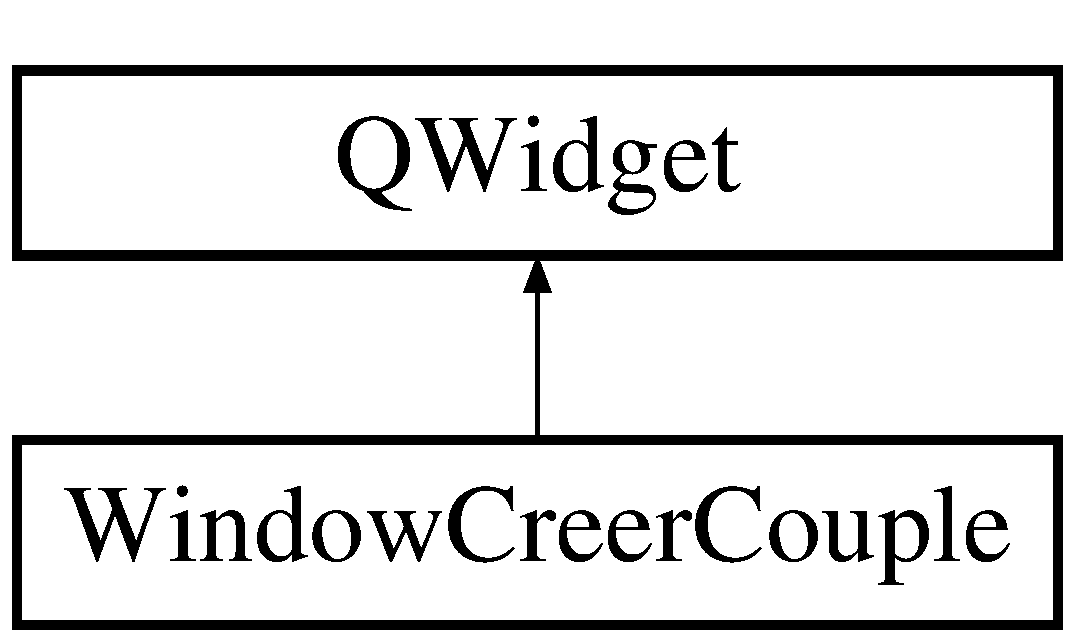
\includegraphics[height=2.000000cm]{class_window_creer_couple}
\end{center}
\end{figure}
\subsection*{Public Member Functions}
\begin{DoxyCompactItemize}
\item 
\mbox{\Hypertarget{class_window_creer_couple_a950f6a9423a2deb211723f551cf61ea2}\label{class_window_creer_couple_a950f6a9423a2deb211723f551cf61ea2}} 
{\bfseries Window\+Creer\+Couple} (Q\+Widget $\ast$parent=0)
\item 
\mbox{\Hypertarget{class_window_creer_couple_a40c809914023acd99e54c14b42a832c9}\label{class_window_creer_couple_a40c809914023acd99e54c14b42a832c9}} 
Q\+Push\+Button $\ast$ {\bfseries get\+Bouton\+Valider} ()
\item 
\mbox{\Hypertarget{class_window_creer_couple_a35e6f537a9f0c5279283240e3e309e77}\label{class_window_creer_couple_a35e6f537a9f0c5279283240e3e309e77}} 
Q\+String {\bfseries get\+Note1} () const
\item 
\mbox{\Hypertarget{class_window_creer_couple_ac824ca2cd99b16928cf4564023a823d5}\label{class_window_creer_couple_ac824ca2cd99b16928cf4564023a823d5}} 
Q\+String {\bfseries get\+Note2} () const
\item 
\mbox{\Hypertarget{class_window_creer_couple_a502a974958e2978266bf57231803915a}\label{class_window_creer_couple_a502a974958e2978266bf57231803915a}} 
Q\+String {\bfseries get\+Label} () const
\end{DoxyCompactItemize}


\subsection{Detailed Description}
Définit la classe \hyperlink{class_window_creer_couple}{Window\+Creer\+Couple} \+: Emplacement pour créer une couple. 

Hérite de Q\+Widget note1 \+: Formulaire identifiant de la note 1 du couple note2 \+: Formulaire identifiant de la note 2 du couple label \+: Formulaire label du couple de la relation valider \+: Bouton valider annuler \+: Bouton annuler 

The documentation for this class was generated from the following files\+:\begin{DoxyCompactItemize}
\item 
wcreercouple.\+h\item 
wcreercouple.\+cpp\end{DoxyCompactItemize}

\hypertarget{class_window_creer_image}{}\section{Window\+Creer\+Image Class Reference}
\label{class_window_creer_image}\index{Window\+Creer\+Image@{Window\+Creer\+Image}}
Inheritance diagram for Window\+Creer\+Image\+:\begin{figure}[H]
\begin{center}
\leavevmode
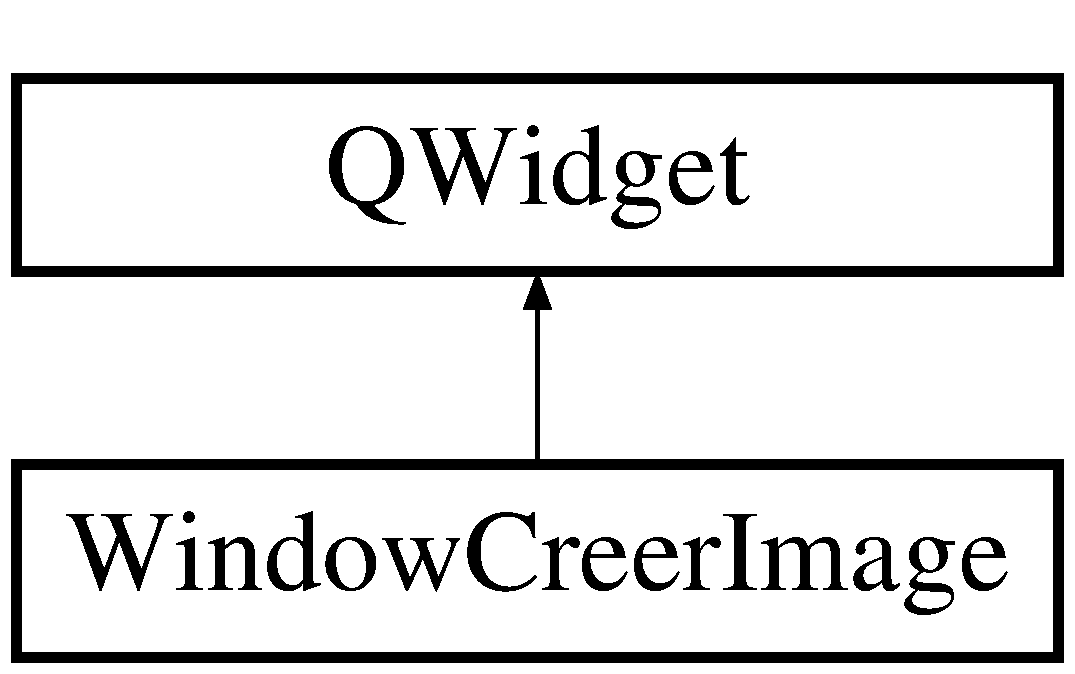
\includegraphics[height=2.000000cm]{class_window_creer_image}
\end{center}
\end{figure}
\subsection*{Public Slots}
\begin{DoxyCompactItemize}
\item 
\mbox{\Hypertarget{class_window_creer_image_a021cfe549b03de190478c16f0a1b07c2}\label{class_window_creer_image_a021cfe549b03de190478c16f0a1b07c2}} 
void \hyperlink{class_window_creer_image_a021cfe549b03de190478c16f0a1b07c2}{create} ()
\begin{DoxyCompactList}\small\item\em Récupère les données du formulaire et créer la note. \end{DoxyCompactList}\end{DoxyCompactItemize}
\subsection*{Public Member Functions}
\begin{DoxyCompactItemize}
\item 
\mbox{\Hypertarget{class_window_creer_image_a2cd80bac4f212bc2abf3dd3b3fdaeb59}\label{class_window_creer_image_a2cd80bac4f212bc2abf3dd3b3fdaeb59}} 
{\bfseries Window\+Creer\+Image} (Q\+String \&ident, Q\+String \&titre, Q\+Widget $\ast$parent=0)
\item 
\mbox{\Hypertarget{class_window_creer_image_aa32a8e392e9c16ec9a634591c87755c4}\label{class_window_creer_image_aa32a8e392e9c16ec9a634591c87755c4}} 
Q\+Push\+Button $\ast$ {\bfseries get\+Button\+Create} ()
\item 
\mbox{\Hypertarget{class_window_creer_image_ad8312e6c9a723333399b0cffc2b308f6}\label{class_window_creer_image_ad8312e6c9a723333399b0cffc2b308f6}} 
Q\+Text\+Edit $\ast$ {\bfseries get\+Desc\+Box} ()
\item 
\mbox{\Hypertarget{class_window_creer_image_a123decae461db49f5542b6229205e2a2}\label{class_window_creer_image_a123decae461db49f5542b6229205e2a2}} 
Q\+Line\+Edit $\ast$ {\bfseries get\+Image\+Box} ()
\end{DoxyCompactItemize}


The documentation for this class was generated from the following files\+:\begin{DoxyCompactItemize}
\item 
\hyperlink{wcreerimage_8h}{wcreerimage.\+h}\item 
wcreerimage.\+cpp\end{DoxyCompactItemize}

\hypertarget{class_window_creer_note}{}\section{Window\+Creer\+Note Class Reference}
\label{class_window_creer_note}\index{Window\+Creer\+Note@{Window\+Creer\+Note}}
Inheritance diagram for Window\+Creer\+Note\+:\begin{figure}[H]
\begin{center}
\leavevmode
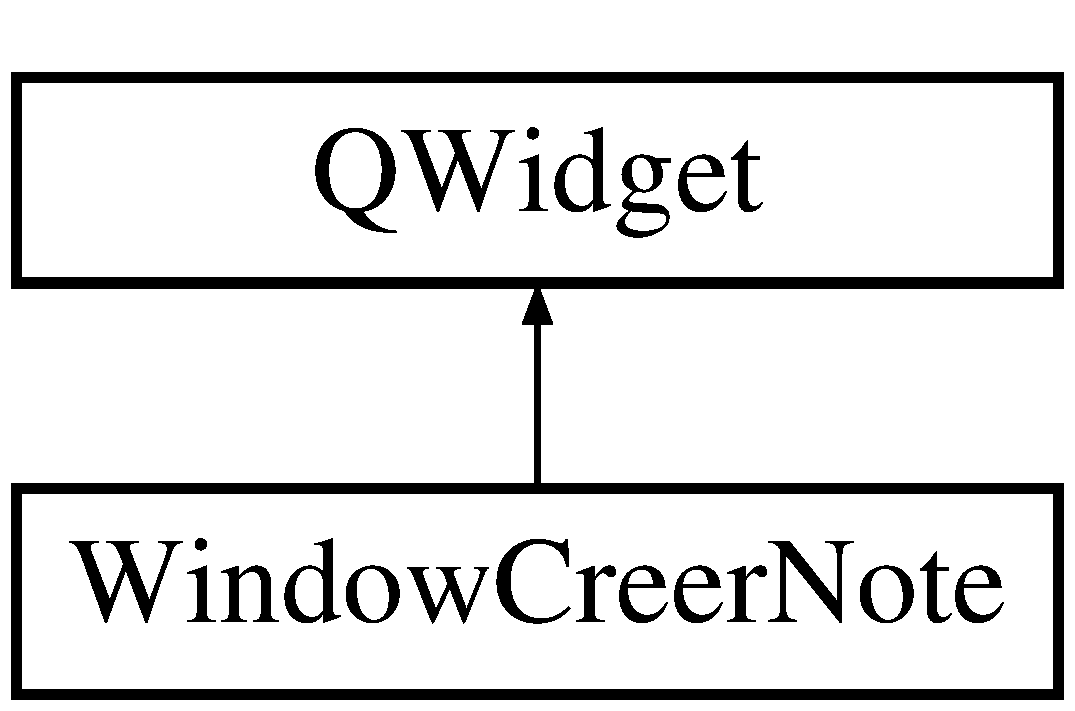
\includegraphics[height=2.000000cm]{class_window_creer_note}
\end{center}
\end{figure}
\subsection*{Public Member Functions}
\begin{DoxyCompactItemize}
\item 
\mbox{\Hypertarget{class_window_creer_note_a1b9d13c3818e450e1d3dffc5707658f4}\label{class_window_creer_note_a1b9d13c3818e450e1d3dffc5707658f4}} 
{\bfseries Window\+Creer\+Note} (Q\+Widget $\ast$parent=0)
\item 
\mbox{\Hypertarget{class_window_creer_note_a036ba88629b9e826fbec74655839a596}\label{class_window_creer_note_a036ba88629b9e826fbec74655839a596}} 
Q\+Combo\+Box $\ast$ {\bfseries get\+Combo\+Type} ()
\item 
\mbox{\Hypertarget{class_window_creer_note_a109db3e13f21dc3ddb1038287fda60a3}\label{class_window_creer_note_a109db3e13f21dc3ddb1038287fda60a3}} 
Q\+Push\+Button $\ast$ {\bfseries get\+Bouton\+Valider} ()
\item 
\mbox{\Hypertarget{class_window_creer_note_aecc75344edf4436802f406f13a47bba7}\label{class_window_creer_note_aecc75344edf4436802f406f13a47bba7}} 
Q\+String {\bfseries get\+Id} () const
\item 
\mbox{\Hypertarget{class_window_creer_note_ad76caab1cd6962d93c855bbb4da6ebf0}\label{class_window_creer_note_ad76caab1cd6962d93c855bbb4da6ebf0}} 
Q\+String {\bfseries get\+Title} () const
\item 
\mbox{\Hypertarget{class_window_creer_note_ade4db2abe278a39b26cd66cc4530ddec}\label{class_window_creer_note_ade4db2abe278a39b26cd66cc4530ddec}} 
Q\+String {\bfseries get\+Type\+Note} () const
\end{DoxyCompactItemize}


The documentation for this class was generated from the following files\+:\begin{DoxyCompactItemize}
\item 
\hyperlink{wcreernote_8h}{wcreernote.\+h}\item 
wcreernote.\+cpp\end{DoxyCompactItemize}

\hypertarget{class_window_creer_relation}{}\section{Window\+Creer\+Relation Class Reference}
\label{class_window_creer_relation}\index{Window\+Creer\+Relation@{Window\+Creer\+Relation}}


Définit la classe \hyperlink{class_window_creer_relation}{Window\+Creer\+Relation} \+: Emplacement pour créer une relation.  




{\ttfamily \#include $<$windowcreerrelation.\+h$>$}

Inheritance diagram for Window\+Creer\+Relation\+:\begin{figure}[H]
\begin{center}
\leavevmode
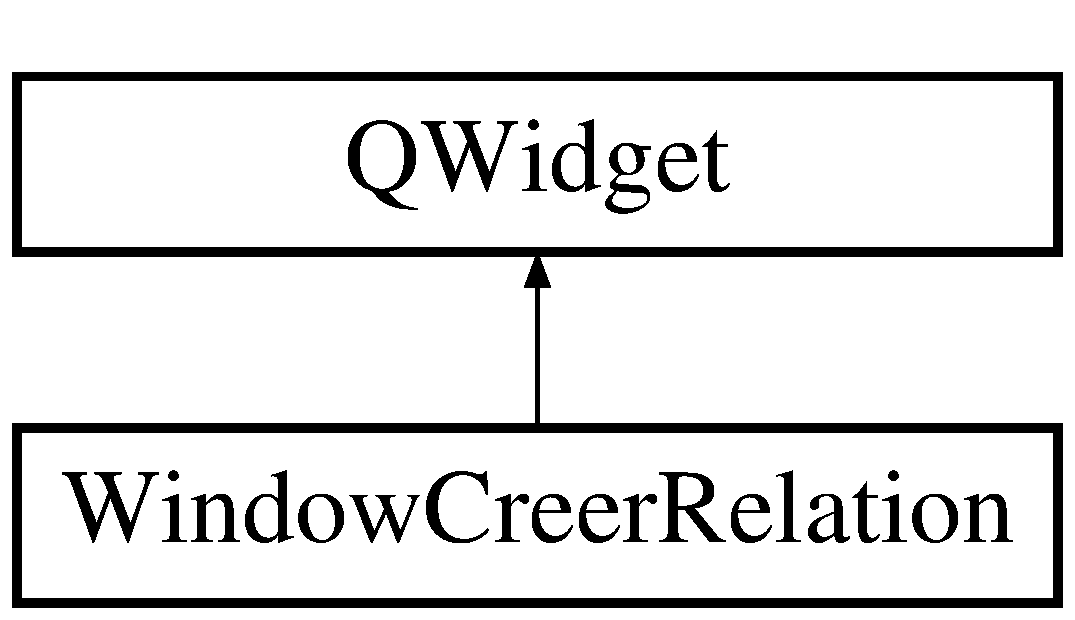
\includegraphics[height=2.000000cm]{class_window_creer_relation}
\end{center}
\end{figure}
\subsection*{Public Member Functions}
\begin{DoxyCompactItemize}
\item 
\mbox{\Hypertarget{class_window_creer_relation_a89501cee057634f9618f1031df95f0ae}\label{class_window_creer_relation_a89501cee057634f9618f1031df95f0ae}} 
{\bfseries Window\+Creer\+Relation} (Q\+Widget $\ast$parent=0)
\item 
\mbox{\Hypertarget{class_window_creer_relation_a0e57f258b6663450dcf4f6d02ff7de36}\label{class_window_creer_relation_a0e57f258b6663450dcf4f6d02ff7de36}} 
Q\+Combo\+Box $\ast$ {\bfseries get\+Combo\+Type} ()
\item 
\mbox{\Hypertarget{class_window_creer_relation_a2998e87a3920cba7a56a56a590752c5d}\label{class_window_creer_relation_a2998e87a3920cba7a56a56a590752c5d}} 
Q\+Push\+Button $\ast$ {\bfseries get\+Bouton\+Valider} ()
\item 
\mbox{\Hypertarget{class_window_creer_relation_a1669245179b6b5d9509ad5080a9dcfa7}\label{class_window_creer_relation_a1669245179b6b5d9509ad5080a9dcfa7}} 
Q\+String {\bfseries get\+Title} () const
\item 
\mbox{\Hypertarget{class_window_creer_relation_a1b195952c535be0f539d6c7b389b8597}\label{class_window_creer_relation_a1b195952c535be0f539d6c7b389b8597}} 
Q\+String {\bfseries get\+Desc} () const
\item 
\mbox{\Hypertarget{class_window_creer_relation_a398c516b68c1e4bab66ce341d7f7fe54}\label{class_window_creer_relation_a398c516b68c1e4bab66ce341d7f7fe54}} 
Q\+String {\bfseries get\+Orientation} () const
\end{DoxyCompactItemize}


\subsection{Detailed Description}
Définit la classe \hyperlink{class_window_creer_relation}{Window\+Creer\+Relation} \+: Emplacement pour créer une relation. 

Hérite de Q\+Widget title\+: Formulaire titre de la relation desc \+: Formulaire description de la relation orientee \+: Formulaire orientation de la relation valider \+: Bouton valider annuler \+: Bouton annuler 

The documentation for this class was generated from the following files\+:\begin{DoxyCompactItemize}
\item 
\hyperlink{windowcreerrelation_8h}{windowcreerrelation.\+h}\item 
windowcreerrelation.\+cpp\end{DoxyCompactItemize}

\hypertarget{class_window_creer_tache}{}\section{Window\+Creer\+Tache Class Reference}
\label{class_window_creer_tache}\index{Window\+Creer\+Tache@{Window\+Creer\+Tache}}
Inheritance diagram for Window\+Creer\+Tache\+:\begin{figure}[H]
\begin{center}
\leavevmode
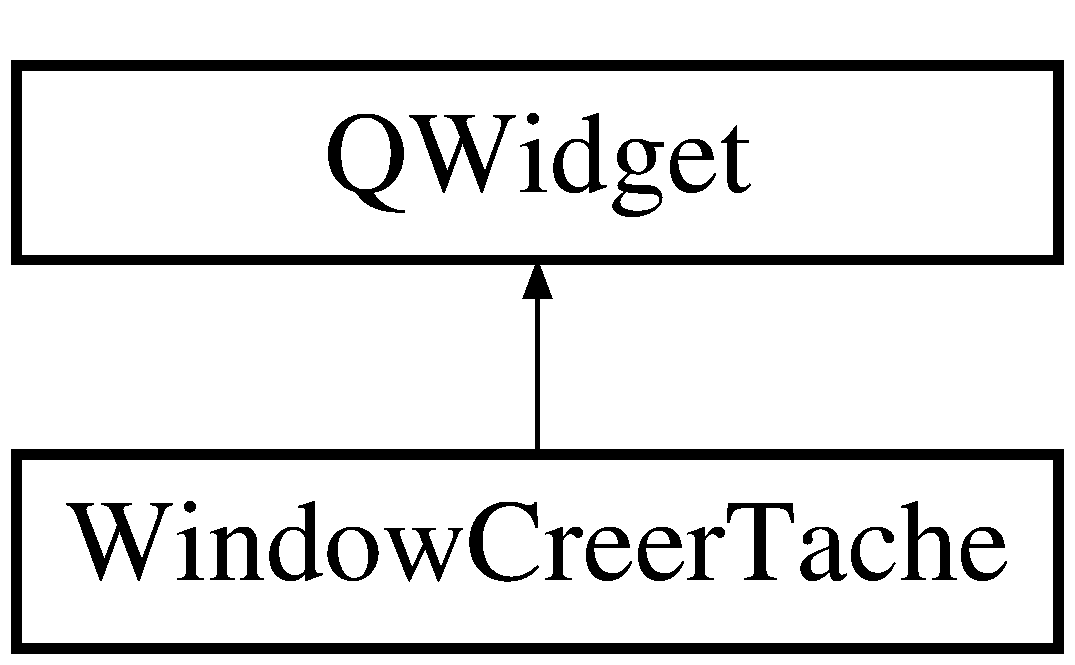
\includegraphics[height=2.000000cm]{class_window_creer_tache}
\end{center}
\end{figure}
\subsection*{Public Slots}
\begin{DoxyCompactItemize}
\item 
\mbox{\Hypertarget{class_window_creer_tache_ad80f952d0e7fc08674a82ed19e94f178}\label{class_window_creer_tache_ad80f952d0e7fc08674a82ed19e94f178}} 
void \hyperlink{class_window_creer_tache_ad80f952d0e7fc08674a82ed19e94f178}{create} ()
\begin{DoxyCompactList}\small\item\em Récupère les données du formulaire et créer la note. \end{DoxyCompactList}\end{DoxyCompactItemize}
\subsection*{Public Member Functions}
\begin{DoxyCompactItemize}
\item 
\mbox{\Hypertarget{class_window_creer_tache_ab15914bdeec16e103baef7c5459a3789}\label{class_window_creer_tache_ab15914bdeec16e103baef7c5459a3789}} 
{\bfseries Window\+Creer\+Tache} (Q\+String \&ident, Q\+String \&titre, Q\+Widget $\ast$parent=0)
\item 
\mbox{\Hypertarget{class_window_creer_tache_a35485f8fc864b06fc51fc80deaa675ec}\label{class_window_creer_tache_a35485f8fc864b06fc51fc80deaa675ec}} 
Q\+Push\+Button $\ast$ {\bfseries get\+Button\+Create} ()
\item 
\mbox{\Hypertarget{class_window_creer_tache_a97c7f8d5fa7511bd52422a1b3195988d}\label{class_window_creer_tache_a97c7f8d5fa7511bd52422a1b3195988d}} 
Q\+Text\+Edit $\ast$ {\bfseries get\+Text\+Box} ()
\item 
\mbox{\Hypertarget{class_window_creer_tache_a4cf25dd76c6f5df7694546afe0708342}\label{class_window_creer_tache_a4cf25dd76c6f5df7694546afe0708342}} 
Q\+Line\+Edit $\ast$ {\bfseries get\+Statut\+Box} ()
\item 
\mbox{\Hypertarget{class_window_creer_tache_a8792e508badea882f18c9d40c2dc6a61}\label{class_window_creer_tache_a8792e508badea882f18c9d40c2dc6a61}} 
Q\+Line\+Edit $\ast$ {\bfseries get\+Prio\+Box} ()
\item 
\mbox{\Hypertarget{class_window_creer_tache_a2e95cafe8191c63dd28b05083a43258a}\label{class_window_creer_tache_a2e95cafe8191c63dd28b05083a43258a}} 
Q\+Line\+Edit $\ast$ {\bfseries get\+Date\+\_\+e\+\_\+\+Day\+Box} ()
\item 
\mbox{\Hypertarget{class_window_creer_tache_a235852531968476fc5330b393d67f0eb}\label{class_window_creer_tache_a235852531968476fc5330b393d67f0eb}} 
Q\+Line\+Edit $\ast$ {\bfseries get\+Date\+\_\+e\+\_\+\+Min\+Box} ()
\end{DoxyCompactItemize}


The documentation for this class was generated from the following files\+:\begin{DoxyCompactItemize}
\item 
\hyperlink{wcreertache_8h}{wcreertache.\+h}\item 
wcreertache.\+cpp\end{DoxyCompactItemize}

\hypertarget{class_window_creer_video}{}\section{Window\+Creer\+Video Class Reference}
\label{class_window_creer_video}\index{Window\+Creer\+Video@{Window\+Creer\+Video}}
Inheritance diagram for Window\+Creer\+Video\+:\begin{figure}[H]
\begin{center}
\leavevmode
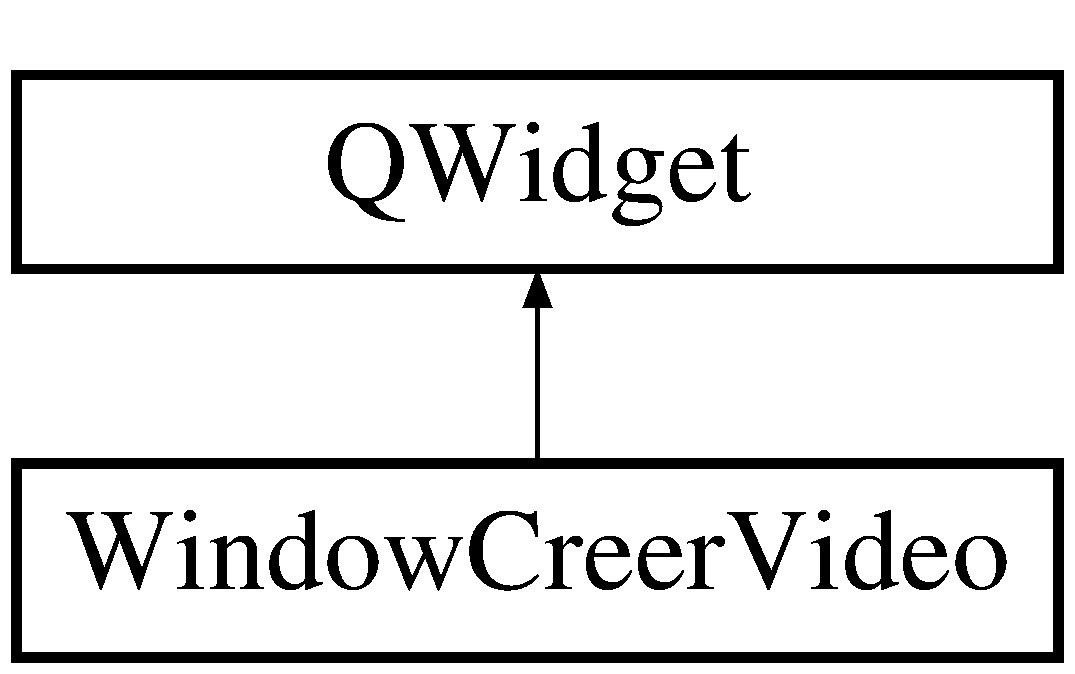
\includegraphics[height=2.000000cm]{class_window_creer_video}
\end{center}
\end{figure}
\subsection*{Public Slots}
\begin{DoxyCompactItemize}
\item 
\mbox{\Hypertarget{class_window_creer_video_ad3e1e8f5e59e2001561e6643d674c351}\label{class_window_creer_video_ad3e1e8f5e59e2001561e6643d674c351}} 
void {\bfseries create} ()
\end{DoxyCompactItemize}
\subsection*{Public Member Functions}
\begin{DoxyCompactItemize}
\item 
\mbox{\Hypertarget{class_window_creer_video_a0e9565a3ecc54a92ed7f713a7994a08d}\label{class_window_creer_video_a0e9565a3ecc54a92ed7f713a7994a08d}} 
{\bfseries Window\+Creer\+Video} (Q\+String \&ident, Q\+String \&titre, Q\+Widget $\ast$parent=0)
\item 
\mbox{\Hypertarget{class_window_creer_video_a60780660a373eda8305b81636456aaaa}\label{class_window_creer_video_a60780660a373eda8305b81636456aaaa}} 
Q\+Push\+Button $\ast$ {\bfseries get\+Button\+Create} ()
\item 
\mbox{\Hypertarget{class_window_creer_video_a0ee2fcb0f619df9f239c3f244df1eb99}\label{class_window_creer_video_a0ee2fcb0f619df9f239c3f244df1eb99}} 
Q\+Text\+Edit $\ast$ {\bfseries get\+Desc\+Box} ()
\item 
\mbox{\Hypertarget{class_window_creer_video_a904f6f5104235bc1d710d8e9eacde6c8}\label{class_window_creer_video_a904f6f5104235bc1d710d8e9eacde6c8}} 
Q\+Line\+Edit $\ast$ {\bfseries get\+Image\+Box} ()
\item 
\mbox{\Hypertarget{class_window_creer_video_a23944954785c8e4187aa92429fd343ce}\label{class_window_creer_video_a23944954785c8e4187aa92429fd343ce}} 
Q\+Line\+Edit $\ast$ {\bfseries get\+Video\+Box} ()
\end{DoxyCompactItemize}


The documentation for this class was generated from the following files\+:\begin{DoxyCompactItemize}
\item 
\hyperlink{wcreervideo_8h}{wcreervideo.\+h}\item 
wcreervideo.\+cpp\end{DoxyCompactItemize}

\hypertarget{class_windowd_creer_image}{}\section{Windowd\+Creer\+Image Class Reference}
\label{class_windowd_creer_image}\index{Windowd\+Creer\+Image@{Windowd\+Creer\+Image}}


Définit la classe \hyperlink{class_windowd_creer_image}{Windowd\+Creer\+Image} \+: Emplacement pour la création d\textquotesingle{}une note image.  




{\ttfamily \#include $<$wcreerimage.\+h$>$}



\subsection{Detailed Description}
Définit la classe \hyperlink{class_windowd_creer_image}{Windowd\+Creer\+Image} \+: Emplacement pour la création d\textquotesingle{}une note image. 

Hérite de Q\+Widget desc\+\_\+box \+: Formulaire description de la image image\+\_\+\+U\+RL \+: Formulaire lien fichier image de la image image\+\_\+title \+: Formulaire titre de la image identifiant \+: Identifiant de la note à créer titre\+\_\+version \+: Titre de la version associée à la note à créer

button\+\_\+create \+: Bouton créer note image button\+\_\+close \+: Bouton fermer 

The documentation for this class was generated from the following file\+:\begin{DoxyCompactItemize}
\item 
\hyperlink{wcreerimage_8h}{wcreerimage.\+h}\end{DoxyCompactItemize}

\hypertarget{class_windowd_creer_note}{}\section{Windowd\+Creer\+Note Class Reference}
\label{class_windowd_creer_note}\index{Windowd\+Creer\+Note@{Windowd\+Creer\+Note}}


Définit la classe \hyperlink{class_windowd_creer_note}{Windowd\+Creer\+Note}\+: Emplacement pour la création d\textquotesingle{}une note.  




{\ttfamily \#include $<$wcreernote.\+h$>$}



\subsection{Detailed Description}
Définit la classe \hyperlink{class_windowd_creer_note}{Windowd\+Creer\+Note}\+: Emplacement pour la création d\textquotesingle{}une note. 

Hérite de Q\+Widget id\+: Formulaire identifiant de la note title \+: Formulaire titre de la version associée à la note type\+\_\+note \+: Formulaire type de la note (\hyperlink{class_article}{Article}, \hyperlink{class_tache}{Tache}, image, video, audio) valider \+: Bouton valider création de la note annuler\+: Bouton annuler 

The documentation for this class was generated from the following file\+:\begin{DoxyCompactItemize}
\item 
\hyperlink{wcreernote_8h}{wcreernote.\+h}\end{DoxyCompactItemize}

\hypertarget{class_windowd_creer_tache}{}\section{Windowd\+Creer\+Tache Class Reference}
\label{class_windowd_creer_tache}\index{Windowd\+Creer\+Tache@{Windowd\+Creer\+Tache}}


Définit la classe \hyperlink{class_windowd_creer_tache}{Windowd\+Creer\+Tache} \+: Emplacement pour la création d\textquotesingle{}une note tâche.  




{\ttfamily \#include $<$wcreertache.\+h$>$}



\subsection{Detailed Description}
Définit la classe \hyperlink{class_windowd_creer_tache}{Windowd\+Creer\+Tache} \+: Emplacement pour la création d\textquotesingle{}une note tâche. 

Hérite de Q\+Widget action\+\_\+box\+: Formulaire action de la tâche statut\+\_\+box \+: Formulaire statut de la tâche prio\+\_\+box \+: Formulaire priorite de la tâche (optionnelle) date\+\_\+e\+\_\+day\+\_\+box \+: Formulaire jour de la date d\textquotesingle{}échéance de la tâche (optionnelle) date\+\_\+e\+\_\+min\+\_\+box \+: Formulaire temps de la date d\textquotesingle{}échéance de la tâche (optionnelle) identifiant \+: Identifiant de la note à créer titre\+\_\+version \+: Titre de la version associée à la note à créer$\ast$ button\+\_\+create \+: Bouton créer note tache button\+\_\+close \+: Bouton fermer 

The documentation for this class was generated from the following file\+:\begin{DoxyCompactItemize}
\item 
\hyperlink{wcreertache_8h}{wcreertache.\+h}\end{DoxyCompactItemize}

\hypertarget{class_windowd_creer_video}{}\section{Windowd\+Creer\+Video Class Reference}
\label{class_windowd_creer_video}\index{Windowd\+Creer\+Video@{Windowd\+Creer\+Video}}


Définit la classe \hyperlink{class_windowd_creer_video}{Windowd\+Creer\+Video} \+: Emplacement pour la création d\textquotesingle{}une note vidéo.  




{\ttfamily \#include $<$wcreervideo.\+h$>$}



\subsection{Detailed Description}
Définit la classe \hyperlink{class_windowd_creer_video}{Windowd\+Creer\+Video} \+: Emplacement pour la création d\textquotesingle{}une note vidéo. 

Hérite de Q\+Widget desc\+\_\+box \+: Formulaire description de la vidéo image\+\_\+\+U\+RL \+: Formulaire lien fichier image de la vidéo video\+\_\+title \+: Formulaire titre de la vidéo identifiant \+: Identifiant de la note à créer titre\+\_\+version \+: Titre de la version associée à la note à créer

button\+\_\+create \+: Bouton créer note vidéo button\+\_\+close \+: Bouton fermer 

The documentation for this class was generated from the following file\+:\begin{DoxyCompactItemize}
\item 
\hyperlink{wcreervideo_8h}{wcreervideo.\+h}\end{DoxyCompactItemize}

\chapter{File Documentation}
\hypertarget{article_8h}{}\section{article.\+h File Reference}
\label{article_8h}\index{article.\+h@{article.\+h}}
{\ttfamily \#include \char`\"{}version.\+h\char`\"{}}\newline
\subsection*{Classes}
\begin{DoxyCompactItemize}
\item 
class \hyperlink{class_article}{Article}
\begin{DoxyCompactList}\small\item\em Définit la classe \hyperlink{class_article}{Article}. \end{DoxyCompactList}\end{DoxyCompactItemize}

\hypertarget{exception_8h}{}\section{exception.\+h File Reference}
\label{exception_8h}\index{exception.\+h@{exception.\+h}}


The exception class.  


{\ttfamily \#include $<$Q\+String$>$}\newline
\subsection*{Classes}
\begin{DoxyCompactItemize}
\item 
class \hyperlink{class_exception}{Exception}
\begin{DoxyCompactList}\small\item\em The \hyperlink{class_exception}{Exception} class\+: class \hyperlink{class_exception}{Exception}. \end{DoxyCompactList}\end{DoxyCompactItemize}


\subsection{Detailed Description}
The exception class. 

\begin{DoxyAuthor}{Author}
Ngo Sy Toan 
\end{DoxyAuthor}
\begin{DoxyDate}{Date}
June 2017 
\end{DoxyDate}

\hypertarget{hafficheraudio_8h}{}\section{hafficheraudio.\+h File Reference}
\label{hafficheraudio_8h}\index{hafficheraudio.\+h@{hafficheraudio.\+h}}
{\ttfamily \#include $<$Q\+Widget$>$}\newline
{\ttfamily \#include $<$Q\+Label$>$}\newline
{\ttfamily \#include $<$Q\+Push\+Button$>$}\newline
{\ttfamily \#include $<$Q\+H\+Box\+Layout$>$}\newline
{\ttfamily \#include $<$Q\+V\+Box\+Layout$>$}\newline
{\ttfamily \#include $<$Q\+Text\+Edit$>$}\newline
{\ttfamily \#include $<$Q\+Line\+Edit$>$}\newline
{\ttfamily \#include \char`\"{}note.\+h\char`\"{}}\newline
{\ttfamily \#include \char`\"{}multimedia.\+h\char`\"{}}\newline
\subsection*{Classes}
\begin{DoxyCompactItemize}
\item 
class \hyperlink{class_window_afficher_audio}{Window\+Afficher\+Audio}
\begin{DoxyCompactList}\small\item\em Définit la classe \hyperlink{class_window_afficher_audio}{Window\+Afficher\+Audio} \+: Emplacement pour afficher un audio. \end{DoxyCompactList}\end{DoxyCompactItemize}

\hypertarget{haffichervideo_8h}{}\section{haffichervideo.\+h File Reference}
\label{haffichervideo_8h}\index{haffichervideo.\+h@{haffichervideo.\+h}}
{\ttfamily \#include $<$Q\+Widget$>$}\newline
{\ttfamily \#include $<$Q\+Label$>$}\newline
{\ttfamily \#include $<$Q\+Push\+Button$>$}\newline
{\ttfamily \#include $<$Q\+H\+Box\+Layout$>$}\newline
{\ttfamily \#include $<$Q\+V\+Box\+Layout$>$}\newline
{\ttfamily \#include $<$Q\+Text\+Edit$>$}\newline
{\ttfamily \#include $<$Q\+Line\+Edit$>$}\newline
{\ttfamily \#include \char`\"{}note.\+h\char`\"{}}\newline
{\ttfamily \#include \char`\"{}multimedia.\+h\char`\"{}}\newline
\subsection*{Classes}
\begin{DoxyCompactItemize}
\item 
class \hyperlink{class_window_afficher_video}{Window\+Afficher\+Video}
\begin{DoxyCompactList}\small\item\em Définit la classe \hyperlink{class_window_afficher_video}{Window\+Afficher\+Video} \+: Emplacement pour afficher un video. \end{DoxyCompactList}\end{DoxyCompactItemize}

\hypertarget{iterator_8h}{}\section{iterator.\+h File Reference}
\label{iterator_8h}\index{iterator.\+h@{iterator.\+h}}


The template of iterator.  


\subsection*{Classes}
\begin{DoxyCompactItemize}
\item 
class \hyperlink{class_iterator}{Iterator$<$ T $>$}
\end{DoxyCompactItemize}


\subsection{Detailed Description}
The template of iterator. 

\begin{DoxyAuthor}{Author}
Ngo Sy Toan 
\end{DoxyAuthor}
\begin{DoxyDate}{Date}
June 2017 
\end{DoxyDate}

\hypertarget{multimedia_8h}{}\section{multimedia.\+h File Reference}
\label{multimedia_8h}\index{multimedia.\+h@{multimedia.\+h}}
{\ttfamily \#include $<$Q\+String$>$}\newline
{\ttfamily \#include $<$Q\+Application$>$}\newline
{\ttfamily \#include $<$Q\+Media\+Player$>$}\newline
{\ttfamily \#include $<$Q\+Pixmap$>$}\newline
{\ttfamily \#include $<$Q\+Label$>$}\newline
{\ttfamily \#include \char`\"{}version.\+h\char`\"{}}\newline
\subsection*{Classes}
\begin{DoxyCompactItemize}
\item 
class \hyperlink{class_multimedia}{Multimedia}
\begin{DoxyCompactList}\small\item\em Définit la classe \hyperlink{class_multimedia}{Multimedia} et ses classes filles (image, audio, video) \end{DoxyCompactList}\item 
class \hyperlink{classimage}{image}
\begin{DoxyCompactList}\small\item\em Classe image hérite de \hyperlink{class_multimedia}{Multimedia}. \end{DoxyCompactList}\item 
class \hyperlink{classaudio}{audio}
\begin{DoxyCompactList}\small\item\em Classe audio hérite de \hyperlink{class_multimedia}{Multimedia}. \end{DoxyCompactList}\item 
class \hyperlink{classvideo}{video}
\begin{DoxyCompactList}\small\item\em Classe video hérite de \hyperlink{class_multimedia}{Multimedia}. \end{DoxyCompactList}\end{DoxyCompactItemize}

\hypertarget{note_8h}{}\section{note.\+h File Reference}
\label{note_8h}\index{note.\+h@{note.\+h}}
{\ttfamily \#include $<$Q\+String$>$}\newline
{\ttfamily \#include $<$Q\+Date\+Time$>$}\newline
{\ttfamily \#include $<$iostream$>$}\newline
{\ttfamily \#include \char`\"{}version.\+h\char`\"{}}\newline
{\ttfamily \#include \char`\"{}iterator.\+h\char`\"{}}\newline
{\ttfamily \#include \char`\"{}exception.\+h\char`\"{}}\newline
\subsection*{Classes}
\begin{DoxyCompactItemize}
\item 
class \hyperlink{class_note}{Note}
\begin{DoxyCompactList}\small\item\em Définit la classe Notes \+: Permet de d\textquotesingle{}ajouter, supprimer, restaurer une \hyperlink{class_version}{Version} à une \hyperlink{class_note}{Note}. \end{DoxyCompactList}\item 
class \hyperlink{class_note_1_1iterator}{Note\+::iterator}
\end{DoxyCompactItemize}
\subsection*{Enumerations}
\begin{DoxyCompactItemize}
\item 
\mbox{\Hypertarget{note_8h_a952f39258bbc825f3d94ffd41440486b}\label{note_8h_a952f39258bbc825f3d94ffd41440486b}} 
enum \hyperlink{note_8h_a952f39258bbc825f3d94ffd41440486b}{Type\+\_\+etat\+\_\+note} \{ {\bfseries active}, 
{\bfseries archive}, 
{\bfseries sursis}
 \}\begin{DoxyCompactList}\small\item\em Enumeration des états des notes

{\itshape active} \+: La note est active {\itshape archive} \+: La note est archivée (supprimée mais encore liée par une relation de Reference) {\itshape sursis} \+: La note est en sursis (supprimée et liée à aucune relation de Reference) \end{DoxyCompactList}
\end{DoxyCompactItemize}
\subsection*{Functions}
\begin{DoxyCompactItemize}
\item 
string \hyperlink{note_8h_a44a4b3e36992ea3a1fe2a252ec7880fa}{enum\+\_\+etat\+\_\+to\+\_\+string} (\hyperlink{note_8h_a952f39258bbc825f3d94ffd41440486b}{Type\+\_\+etat\+\_\+note} t)
\begin{DoxyCompactList}\small\item\em \+: Convertit un Type\+\_\+etat\+\_\+note vers une string. \end{DoxyCompactList}\item 
\hyperlink{note_8h_a952f39258bbc825f3d94ffd41440486b}{Type\+\_\+etat\+\_\+note} \hyperlink{note_8h_acdaea2b0c1efc48920d20c9176cf0503}{string\+\_\+to\+\_\+enum\+\_\+etat} (const string \&s)
\begin{DoxyCompactList}\small\item\em Convertit une string vers un Type\+\_\+etat\+\_\+note. \end{DoxyCompactList}\end{DoxyCompactItemize}


\subsection{Function Documentation}
\mbox{\Hypertarget{note_8h_a44a4b3e36992ea3a1fe2a252ec7880fa}\label{note_8h_a44a4b3e36992ea3a1fe2a252ec7880fa}} 
\index{note.\+h@{note.\+h}!enum\+\_\+etat\+\_\+to\+\_\+string@{enum\+\_\+etat\+\_\+to\+\_\+string}}
\index{enum\+\_\+etat\+\_\+to\+\_\+string@{enum\+\_\+etat\+\_\+to\+\_\+string}!note.\+h@{note.\+h}}
\subsubsection{\texorpdfstring{enum\+\_\+etat\+\_\+to\+\_\+string()}{enum\_etat\_to\_string()}}
{\footnotesize\ttfamily string enum\+\_\+etat\+\_\+to\+\_\+string (\begin{DoxyParamCaption}\item[{\hyperlink{note_8h_a952f39258bbc825f3d94ffd41440486b}{Type\+\_\+etat\+\_\+note}}]{t }\end{DoxyParamCaption})}



\+: Convertit un Type\+\_\+etat\+\_\+note vers une string. 


\begin{DoxyParams}{Parameters}
{\em t} & \+: enum à convertir \\
\hline
\end{DoxyParams}
\begin{DoxyReturn}{Returns}
string de l\textquotesingle{}enum 
\end{DoxyReturn}
\mbox{\Hypertarget{note_8h_acdaea2b0c1efc48920d20c9176cf0503}\label{note_8h_acdaea2b0c1efc48920d20c9176cf0503}} 
\index{note.\+h@{note.\+h}!string\+\_\+to\+\_\+enum\+\_\+etat@{string\+\_\+to\+\_\+enum\+\_\+etat}}
\index{string\+\_\+to\+\_\+enum\+\_\+etat@{string\+\_\+to\+\_\+enum\+\_\+etat}!note.\+h@{note.\+h}}
\subsubsection{\texorpdfstring{string\+\_\+to\+\_\+enum\+\_\+etat()}{string\_to\_enum\_etat()}}
{\footnotesize\ttfamily \hyperlink{note_8h_a952f39258bbc825f3d94ffd41440486b}{Type\+\_\+etat\+\_\+note} string\+\_\+to\+\_\+enum\+\_\+etat (\begin{DoxyParamCaption}\item[{const string \&}]{s }\end{DoxyParamCaption})}



Convertit une string vers un Type\+\_\+etat\+\_\+note. 


\begin{DoxyParams}{Parameters}
{\em s} & \+: string à convertir \\
\hline
\end{DoxyParams}
\begin{DoxyReturn}{Returns}
enum de la string 
\end{DoxyReturn}

\hypertarget{notesmanager_8h}{}\section{notesmanager.\+h File Reference}
\label{notesmanager_8h}\index{notesmanager.\+h@{notesmanager.\+h}}
{\ttfamily \#include \char`\"{}note.\+h\char`\"{}}\newline
{\ttfamily \#include $<$Q\+String$>$}\newline
{\ttfamily \#include $<$Q\+Debug$>$}\newline
{\ttfamily \#include \char`\"{}iterator.\+h\char`\"{}}\newline
{\ttfamily \#include \char`\"{}version.\+h\char`\"{}}\newline
{\ttfamily \#include \char`\"{}relation.\+h\char`\"{}}\newline
{\ttfamily \#include \char`\"{}notesmanager.\+h\char`\"{}}\newline
{\ttfamily \#include $<$Qstring$>$}\newline
{\ttfamily \#include $<$Q\+File$>$}\newline
{\ttfamily \#include $<$Q\+Xml\+Stream\+Writer$>$}\newline
{\ttfamily \#include $<$Q\+Xml\+Stream\+Reader$>$}\newline
\subsection*{Classes}
\begin{DoxyCompactItemize}
\item 
class \hyperlink{class_notes_manager}{Notes\+Manager}
\begin{DoxyCompactList}\small\item\em Définit la classe \hyperlink{class_notes_manager}{Notes\+Manager} \+: Permet de d\textquotesingle{}ajouter, supprimer, restaurer une \hyperlink{class_note}{Note}. Permet de sauvegarder/charger la session dans/à partir d\textquotesingle{}un fichier X\+ML. \end{DoxyCompactList}\item 
class \hyperlink{class_notes_manager_1_1iterator}{Notes\+Manager\+::iterator}
\end{DoxyCompactItemize}

\hypertarget{relation_8h}{}\section{relation.\+h File Reference}
\label{relation_8h}\index{relation.\+h@{relation.\+h}}


The relation file\+: contain all the description of a relation, couple and \hyperlink{class_relation}{Relation} Manager.  


{\ttfamily \#include \char`\"{}note.\+h\char`\"{}}\newline
{\ttfamily \#include \char`\"{}iterator.\+h\char`\"{}}\newline
{\ttfamily \#include $<$Q\+String$>$}\newline
{\ttfamily \#include \char`\"{}exception.\+h\char`\"{}}\newline
\subsection*{Classes}
\begin{DoxyCompactItemize}
\item 
class \hyperlink{class_couple}{Couple}
\begin{DoxyCompactList}\small\item\em The \hyperlink{class_couple}{Couple} class\+: contain 2 note linked together by a relation, with label. \end{DoxyCompactList}\item 
class \hyperlink{class_relation}{Relation}
\begin{DoxyCompactList}\small\item\em The \hyperlink{class_relation}{Relation} class is abstract, it contains couples and the orientation of the couples inside. \end{DoxyCompactList}\item 
class \hyperlink{class_relation_1_1iterator}{Relation\+::iterator}
\begin{DoxyCompactList}\small\item\em The iterator class\+: iterator of relation, iterate throught the table of couple. \end{DoxyCompactList}\item 
class \hyperlink{class_relation_normale}{Relation\+Normale}
\begin{DoxyCompactList}\small\item\em The \hyperlink{class_relation_normale}{Relation\+Normale} class\+: heritate of \hyperlink{class_relation}{Relation} class. \end{DoxyCompactList}\item 
class \hyperlink{class_relation_preexistente}{Relation\+Preexistente}
\begin{DoxyCompactList}\small\item\em The \hyperlink{class_relation_preexistente}{Relation\+Preexistente} class\+: the Preexistence class, Reference. \end{DoxyCompactList}\item 
class \hyperlink{class_relation_manager}{Relation\+Manager}
\begin{DoxyCompactList}\small\item\em The \hyperlink{class_relation_manager}{Relation\+Manager} class\+: \hyperlink{class_relation}{Relation} Manager to manage \hyperlink{class_relation}{Relation}, Singleton. \end{DoxyCompactList}\item 
class \hyperlink{class_relation_manager_1_1iterator}{Relation\+Manager\+::iterator}
\begin{DoxyCompactList}\small\item\em The iterator class\+: iterator through table of relations. \end{DoxyCompactList}\end{DoxyCompactItemize}


\subsection{Detailed Description}
The relation file\+: contain all the description of a relation, couple and \hyperlink{class_relation}{Relation} Manager. 

\begin{DoxyAuthor}{Author}
Ngo Sy Toan 
\end{DoxyAuthor}
\begin{DoxyDate}{Date}
June 2017 
\end{DoxyDate}

\hypertarget{tache_8h}{}\section{tache.\+h File Reference}
\label{tache_8h}\index{tache.\+h@{tache.\+h}}
{\ttfamily \#include \char`\"{}version.\+h\char`\"{}}\newline
{\ttfamily \#include $<$Q\+Date\+Time$>$}\newline
{\ttfamily \#include $<$iostream$>$}\newline
\subsection*{Classes}
\begin{DoxyCompactItemize}
\item 
class \hyperlink{class_tache}{Tache}
\begin{DoxyCompactList}\small\item\em Définit la classe \hyperlink{class_tache}{Tache}. \end{DoxyCompactList}\end{DoxyCompactItemize}
\subsection*{Enumerations}
\begin{DoxyCompactItemize}
\item 
\mbox{\Hypertarget{tache_8h_addeb79f2c3a0b32730bfe5fe5eb962a7}\label{tache_8h_addeb79f2c3a0b32730bfe5fe5eb962a7}} 
enum \hyperlink{tache_8h_addeb79f2c3a0b32730bfe5fe5eb962a7}{Type\+\_\+statut\+\_\+tache} \{ {\bfseries en\+\_\+cours}, 
{\bfseries attente}, 
{\bfseries terminee}
 \}\begin{DoxyCompactList}\small\item\em Enumeration des statut des tâches

{\itshape en\+\_\+cours} \+: La tache est en cours. {\itshape attente} \+: La tache est en attente (par défaut). {\itshape terminee} \+: La tache est en terminée. \end{DoxyCompactList}
\end{DoxyCompactItemize}
\subsection*{Functions}
\begin{DoxyCompactItemize}
\item 
string \hyperlink{tache_8h_ab21b967fc0cce1c56c019ece61ab5fb9}{enum\+\_\+statut\+\_\+to\+\_\+string} (\hyperlink{tache_8h_addeb79f2c3a0b32730bfe5fe5eb962a7}{Type\+\_\+statut\+\_\+tache} t)
\begin{DoxyCompactList}\small\item\em \+: Convertit un Type\+\_\+statut\+\_\+tache vers une string. \end{DoxyCompactList}\item 
\hyperlink{tache_8h_addeb79f2c3a0b32730bfe5fe5eb962a7}{Type\+\_\+statut\+\_\+tache} \hyperlink{tache_8h_a93584148c485123af15a068a269fc628}{string\+\_\+to\+\_\+enum\+\_\+statut} (const string \&s)
\begin{DoxyCompactList}\small\item\em Convertit une string vers un Type\+\_\+statut\+\_\+tache. \end{DoxyCompactList}\item 
Q\+String \hyperlink{tache_8h_a5830a98d0d3eab8bb3f2ca3845c756ed}{enum\+\_\+statut\+\_\+to\+\_\+qstring} (\hyperlink{tache_8h_addeb79f2c3a0b32730bfe5fe5eb962a7}{Type\+\_\+statut\+\_\+tache} t)
\begin{DoxyCompactList}\small\item\em \+: Convertit un Type\+\_\+statut\+\_\+tache vers une string. \end{DoxyCompactList}\item 
\hyperlink{tache_8h_addeb79f2c3a0b32730bfe5fe5eb962a7}{Type\+\_\+statut\+\_\+tache} \hyperlink{tache_8h_a21959831415f2c105008f9c6d5440f55}{qstring\+\_\+to\+\_\+enum\+\_\+statut} (const Q\+String \&s)
\begin{DoxyCompactList}\small\item\em Convertit une string vers un Type\+\_\+statut\+\_\+tache. \end{DoxyCompactList}\end{DoxyCompactItemize}


\subsection{Function Documentation}
\mbox{\Hypertarget{tache_8h_a5830a98d0d3eab8bb3f2ca3845c756ed}\label{tache_8h_a5830a98d0d3eab8bb3f2ca3845c756ed}} 
\index{tache.\+h@{tache.\+h}!enum\+\_\+statut\+\_\+to\+\_\+qstring@{enum\+\_\+statut\+\_\+to\+\_\+qstring}}
\index{enum\+\_\+statut\+\_\+to\+\_\+qstring@{enum\+\_\+statut\+\_\+to\+\_\+qstring}!tache.\+h@{tache.\+h}}
\subsubsection{\texorpdfstring{enum\+\_\+statut\+\_\+to\+\_\+qstring()}{enum\_statut\_to\_qstring()}}
{\footnotesize\ttfamily Q\+String enum\+\_\+statut\+\_\+to\+\_\+qstring (\begin{DoxyParamCaption}\item[{\hyperlink{tache_8h_addeb79f2c3a0b32730bfe5fe5eb962a7}{Type\+\_\+statut\+\_\+tache}}]{t }\end{DoxyParamCaption})}



\+: Convertit un Type\+\_\+statut\+\_\+tache vers une string. 


\begin{DoxyParams}{Parameters}
{\em t} & \+: enum à convertir \\
\hline
\end{DoxyParams}
\begin{DoxyReturn}{Returns}
Qstring de l\textquotesingle{}enum 
\end{DoxyReturn}
\mbox{\Hypertarget{tache_8h_ab21b967fc0cce1c56c019ece61ab5fb9}\label{tache_8h_ab21b967fc0cce1c56c019ece61ab5fb9}} 
\index{tache.\+h@{tache.\+h}!enum\+\_\+statut\+\_\+to\+\_\+string@{enum\+\_\+statut\+\_\+to\+\_\+string}}
\index{enum\+\_\+statut\+\_\+to\+\_\+string@{enum\+\_\+statut\+\_\+to\+\_\+string}!tache.\+h@{tache.\+h}}
\subsubsection{\texorpdfstring{enum\+\_\+statut\+\_\+to\+\_\+string()}{enum\_statut\_to\_string()}}
{\footnotesize\ttfamily string enum\+\_\+statut\+\_\+to\+\_\+string (\begin{DoxyParamCaption}\item[{\hyperlink{tache_8h_addeb79f2c3a0b32730bfe5fe5eb962a7}{Type\+\_\+statut\+\_\+tache}}]{t }\end{DoxyParamCaption})}



\+: Convertit un Type\+\_\+statut\+\_\+tache vers une string. 


\begin{DoxyParams}{Parameters}
{\em t} & \+: enum à convertir \\
\hline
\end{DoxyParams}
\begin{DoxyReturn}{Returns}
string de l\textquotesingle{}enum 
\end{DoxyReturn}
\mbox{\Hypertarget{tache_8h_a21959831415f2c105008f9c6d5440f55}\label{tache_8h_a21959831415f2c105008f9c6d5440f55}} 
\index{tache.\+h@{tache.\+h}!qstring\+\_\+to\+\_\+enum\+\_\+statut@{qstring\+\_\+to\+\_\+enum\+\_\+statut}}
\index{qstring\+\_\+to\+\_\+enum\+\_\+statut@{qstring\+\_\+to\+\_\+enum\+\_\+statut}!tache.\+h@{tache.\+h}}
\subsubsection{\texorpdfstring{qstring\+\_\+to\+\_\+enum\+\_\+statut()}{qstring\_to\_enum\_statut()}}
{\footnotesize\ttfamily \hyperlink{tache_8h_addeb79f2c3a0b32730bfe5fe5eb962a7}{Type\+\_\+statut\+\_\+tache} qstring\+\_\+to\+\_\+enum\+\_\+statut (\begin{DoxyParamCaption}\item[{const Q\+String \&}]{s }\end{DoxyParamCaption})}



Convertit une string vers un Type\+\_\+statut\+\_\+tache. 


\begin{DoxyParams}{Parameters}
{\em s} & \+: Qstring à convertir \\
\hline
\end{DoxyParams}
\begin{DoxyReturn}{Returns}
enum de la string 
\end{DoxyReturn}
\mbox{\Hypertarget{tache_8h_a93584148c485123af15a068a269fc628}\label{tache_8h_a93584148c485123af15a068a269fc628}} 
\index{tache.\+h@{tache.\+h}!string\+\_\+to\+\_\+enum\+\_\+statut@{string\+\_\+to\+\_\+enum\+\_\+statut}}
\index{string\+\_\+to\+\_\+enum\+\_\+statut@{string\+\_\+to\+\_\+enum\+\_\+statut}!tache.\+h@{tache.\+h}}
\subsubsection{\texorpdfstring{string\+\_\+to\+\_\+enum\+\_\+statut()}{string\_to\_enum\_statut()}}
{\footnotesize\ttfamily \hyperlink{tache_8h_addeb79f2c3a0b32730bfe5fe5eb962a7}{Type\+\_\+statut\+\_\+tache} string\+\_\+to\+\_\+enum\+\_\+statut (\begin{DoxyParamCaption}\item[{const string \&}]{s }\end{DoxyParamCaption})}



Convertit une string vers un Type\+\_\+statut\+\_\+tache. 


\begin{DoxyParams}{Parameters}
{\em s} & \+: string à convertir \\
\hline
\end{DoxyParams}
\begin{DoxyReturn}{Returns}
enum de la string 
\end{DoxyReturn}

\hypertarget{version_8h}{}\section{version.\+h File Reference}
\label{version_8h}\index{version.\+h@{version.\+h}}
{\ttfamily \#include $<$Q\+String$>$}\newline
{\ttfamily \#include $<$Q\+Date\+Time$>$}\newline
{\ttfamily \#include $<$Q\+Date$>$}\newline
{\ttfamily \#include $<$Q\+Time$>$}\newline
{\ttfamily \#include \char`\"{}exception.\+h\char`\"{}}\newline
\subsection*{Classes}
\begin{DoxyCompactItemize}
\item 
class \hyperlink{class_version}{Version}
\begin{DoxyCompactList}\small\item\em Définit la classe \hyperlink{class_version}{Version}. \end{DoxyCompactList}\end{DoxyCompactItemize}

\hypertarget{wafficherarticle_8h}{}\section{wafficherarticle.\+h File Reference}
\label{wafficherarticle_8h}\index{wafficherarticle.\+h@{wafficherarticle.\+h}}


The widget to view and edit article.  


{\ttfamily \#include $<$Q\+Widget$>$}\newline
{\ttfamily \#include $<$Q\+Label$>$}\newline
{\ttfamily \#include $<$Q\+Push\+Button$>$}\newline
{\ttfamily \#include $<$Q\+H\+Box\+Layout$>$}\newline
{\ttfamily \#include $<$Q\+V\+Box\+Layout$>$}\newline
{\ttfamily \#include $<$Q\+Text\+Edit$>$}\newline
{\ttfamily \#include $<$Q\+Line\+Edit$>$}\newline
{\ttfamily \#include \char`\"{}article.\+h\char`\"{}}\newline
{\ttfamily \#include \char`\"{}note.\+h\char`\"{}}\newline
\subsection*{Classes}
\begin{DoxyCompactItemize}
\item 
class \hyperlink{class_window_afficher_article}{Window\+Afficher\+Article}
\begin{DoxyCompactList}\small\item\em The \hyperlink{class_window_afficher_article}{Window\+Afficher\+Article} class\+: Widget to view and edit article. \end{DoxyCompactList}\end{DoxyCompactItemize}


\subsection{Detailed Description}
The widget to view and edit article. 

\begin{DoxyAuthor}{Author}
Ngo Sy Toan 
\end{DoxyAuthor}
\begin{DoxyDate}{Date}
June 2017 
\end{DoxyDate}

\hypertarget{waffichercouple_8h}{}\section{waffichercouple.\+h File Reference}
\label{waffichercouple_8h}\index{waffichercouple.\+h@{waffichercouple.\+h}}


The widget to view all couples of a relation.  


{\ttfamily \#include $<$Q\+Widget$>$}\newline
{\ttfamily \#include $<$Q\+Label$>$}\newline
{\ttfamily \#include $<$Q\+Push\+Button$>$}\newline
{\ttfamily \#include $<$Q\+H\+Box\+Layout$>$}\newline
{\ttfamily \#include $<$Q\+V\+Box\+Layout$>$}\newline
{\ttfamily \#include $<$Q\+Text\+Edit$>$}\newline
{\ttfamily \#include $<$Q\+List\+Widget$>$}\newline
{\ttfamily \#include $<$Q\+Layout$>$}\newline
{\ttfamily \#include \char`\"{}relation.\+h\char`\"{}}\newline
\subsection*{Classes}
\begin{DoxyCompactItemize}
\item 
class \hyperlink{class_window_afficher_couple}{Window\+Afficher\+Couple}
\begin{DoxyCompactList}\small\item\em The \hyperlink{class_window_afficher_couple}{Window\+Afficher\+Couple} class\+: the Widget to view all couplees of a relation. \end{DoxyCompactList}\end{DoxyCompactItemize}


\subsection{Detailed Description}
The widget to view all couples of a relation. 

\begin{DoxyAuthor}{Author}
Ngo Sy Toan 
\end{DoxyAuthor}
\begin{DoxyDate}{Date}
June 2017 
\end{DoxyDate}

\hypertarget{wafficherimage_8h}{}\section{wafficherimage.\+h File Reference}
\label{wafficherimage_8h}\index{wafficherimage.\+h@{wafficherimage.\+h}}


The widget to view view and edit image.  


{\ttfamily \#include $<$Q\+Widget$>$}\newline
{\ttfamily \#include $<$Q\+Label$>$}\newline
{\ttfamily \#include $<$Q\+Push\+Button$>$}\newline
{\ttfamily \#include $<$Q\+H\+Box\+Layout$>$}\newline
{\ttfamily \#include $<$Q\+V\+Box\+Layout$>$}\newline
{\ttfamily \#include $<$Q\+Text\+Edit$>$}\newline
{\ttfamily \#include $<$Q\+Line\+Edit$>$}\newline
{\ttfamily \#include \char`\"{}note.\+h\char`\"{}}\newline
{\ttfamily \#include \char`\"{}multimedia.\+h\char`\"{}}\newline
\subsection*{Classes}
\begin{DoxyCompactItemize}
\item 
class \hyperlink{class_window_afficher_image}{Window\+Afficher\+Image}
\begin{DoxyCompactList}\small\item\em The Window\+Afficher\+Imag class\+: Widget to view and edit image. \end{DoxyCompactList}\end{DoxyCompactItemize}


\subsection{Detailed Description}
The widget to view view and edit image. 

\begin{DoxyAuthor}{Author}
Ngo Sy Toan 
\end{DoxyAuthor}
\begin{DoxyDate}{Date}
June 2017 
\end{DoxyDate}

\hypertarget{waffichertache_8h}{}\section{waffichertache.\+h File Reference}
\label{waffichertache_8h}\index{waffichertache.\+h@{waffichertache.\+h}}


The widget to view and edit tache.  


{\ttfamily \#include $<$Q\+Widget$>$}\newline
{\ttfamily \#include $<$Q\+Label$>$}\newline
{\ttfamily \#include $<$Q\+Push\+Button$>$}\newline
{\ttfamily \#include $<$Q\+H\+Box\+Layout$>$}\newline
{\ttfamily \#include $<$Q\+V\+Box\+Layout$>$}\newline
{\ttfamily \#include $<$Q\+Text\+Edit$>$}\newline
{\ttfamily \#include $<$Q\+Line\+Edit$>$}\newline
{\ttfamily \#include $<$Q\+String$>$}\newline
{\ttfamily \#include $<$Q\+Date\+Time$>$}\newline
{\ttfamily \#include \char`\"{}note.\+h\char`\"{}}\newline
{\ttfamily \#include \char`\"{}version.\+h\char`\"{}}\newline
{\ttfamily \#include \char`\"{}tache.\+h\char`\"{}}\newline
\subsection*{Classes}
\begin{DoxyCompactItemize}
\item 
class \hyperlink{class_window_afficher_tache}{Window\+Afficher\+Tache}
\end{DoxyCompactItemize}


\subsection{Detailed Description}
The widget to view and edit tache. 

\begin{DoxyAuthor}{Author}
Ngo Sy Toan 
\end{DoxyAuthor}
\begin{DoxyDate}{Date}
June 2017 
\end{DoxyDate}

\hypertarget{warborescence_8h}{}\section{warborescence.\+h File Reference}
\label{warborescence_8h}\index{warborescence.\+h@{warborescence.\+h}}


The widget to view arborescence.  


{\ttfamily \#include $<$Q\+Widget$>$}\newline
\subsection*{Classes}
\begin{DoxyCompactItemize}
\item 
class \hyperlink{class_droite_arborescence}{Droite\+Arborescence}
\begin{DoxyCompactList}\small\item\em The \hyperlink{class_droite_arborescence}{Droite\+Arborescence} class\+: Widget to view arborescence. \end{DoxyCompactList}\end{DoxyCompactItemize}


\subsection{Detailed Description}
The widget to view arborescence. 

\begin{DoxyAuthor}{Author}
Ngo Sy Toan 
\end{DoxyAuthor}
\begin{DoxyDate}{Date}
June 2017 
\end{DoxyDate}

\hypertarget{wcreerarticle_8h}{}\section{wcreerarticle.\+h File Reference}
\label{wcreerarticle_8h}\index{wcreerarticle.\+h@{wcreerarticle.\+h}}


The widget to create new article.  


{\ttfamily \#include $<$Q\+Widget$>$}\newline
{\ttfamily \#include $<$Q\+Label$>$}\newline
{\ttfamily \#include $<$Q\+Push\+Button$>$}\newline
{\ttfamily \#include $<$Q\+H\+Box\+Layout$>$}\newline
{\ttfamily \#include $<$Q\+V\+Box\+Layout$>$}\newline
{\ttfamily \#include $<$Q\+Text\+Edit$>$}\newline
\subsection*{Classes}
\begin{DoxyCompactItemize}
\item 
class \hyperlink{class_window_creer_article}{Window\+Creer\+Article}
\begin{DoxyCompactList}\small\item\em The \hyperlink{class_window_creer_article}{Window\+Creer\+Article} class\+: Widget to create new article. \end{DoxyCompactList}\end{DoxyCompactItemize}


\subsection{Detailed Description}
The widget to create new article. 

\begin{DoxyAuthor}{Author}
Ngo Sy Toan 
\end{DoxyAuthor}
\begin{DoxyDate}{Date}
June 2017 
\end{DoxyDate}

\hypertarget{wcreeraudio_8h}{}\section{wcreeraudio.\+h File Reference}
\label{wcreeraudio_8h}\index{wcreeraudio.\+h@{wcreeraudio.\+h}}


The widget to create audio.  


{\ttfamily \#include $<$Q\+Widget$>$}\newline
{\ttfamily \#include $<$Q\+Label$>$}\newline
{\ttfamily \#include $<$Q\+Push\+Button$>$}\newline
{\ttfamily \#include $<$Q\+H\+Box\+Layout$>$}\newline
{\ttfamily \#include $<$Q\+V\+Box\+Layout$>$}\newline
{\ttfamily \#include $<$Q\+Text\+Edit$>$}\newline
{\ttfamily \#include $<$Q\+Line\+Edit$>$}\newline
\subsection*{Classes}
\begin{DoxyCompactItemize}
\item 
class \hyperlink{class_window_creer_audio}{Window\+Creer\+Audio}
\begin{DoxyCompactList}\small\item\em The \hyperlink{class_window_creer_audio}{Window\+Creer\+Audio} class\+: Widget to create new audio. \end{DoxyCompactList}\end{DoxyCompactItemize}


\subsection{Detailed Description}
The widget to create audio. 

\begin{DoxyAuthor}{Author}
Ngo Sy Toan 
\end{DoxyAuthor}
\begin{DoxyDate}{Date}
June 2017 
\end{DoxyDate}

\hypertarget{wcreerimage_8h}{}\section{wcreerimage.\+h File Reference}
\label{wcreerimage_8h}\index{wcreerimage.\+h@{wcreerimage.\+h}}
{\ttfamily \#include $<$Q\+Widget$>$}\newline
{\ttfamily \#include $<$Q\+Label$>$}\newline
{\ttfamily \#include $<$Q\+Push\+Button$>$}\newline
{\ttfamily \#include $<$Q\+H\+Box\+Layout$>$}\newline
{\ttfamily \#include $<$Q\+V\+Box\+Layout$>$}\newline
{\ttfamily \#include $<$Q\+Text\+Edit$>$}\newline
{\ttfamily \#include $<$Q\+Line\+Edit$>$}\newline
\subsection*{Classes}
\begin{DoxyCompactItemize}
\item 
class \hyperlink{class_window_creer_image}{Window\+Creer\+Image}
\end{DoxyCompactItemize}

\hypertarget{wcreernote_8h}{}\section{wcreernote.\+h File Reference}
\label{wcreernote_8h}\index{wcreernote.\+h@{wcreernote.\+h}}
{\ttfamily \#include $<$Q\+Widget$>$}\newline
{\ttfamily \#include $<$Q\+Combo\+Box$>$}\newline
{\ttfamily \#include $<$Q\+Label$>$}\newline
{\ttfamily \#include $<$Q\+Push\+Button$>$}\newline
{\ttfamily \#include $<$Q\+H\+Box\+Layout$>$}\newline
{\ttfamily \#include $<$Q\+Form\+Layout$>$}\newline
{\ttfamily \#include \char`\"{}wcreerarticle.\+h\char`\"{}}\newline
{\ttfamily \#include $<$Q\+Line\+Edit$>$}\newline
\subsection*{Classes}
\begin{DoxyCompactItemize}
\item 
class \hyperlink{class_window_creer_note}{Window\+Creer\+Note}
\end{DoxyCompactItemize}

\hypertarget{wcreertache_8h}{}\section{wcreertache.\+h File Reference}
\label{wcreertache_8h}\index{wcreertache.\+h@{wcreertache.\+h}}
{\ttfamily \#include $<$Q\+Widget$>$}\newline
{\ttfamily \#include $<$Q\+Label$>$}\newline
{\ttfamily \#include $<$Q\+Push\+Button$>$}\newline
{\ttfamily \#include $<$Q\+H\+Box\+Layout$>$}\newline
{\ttfamily \#include $<$Q\+V\+Box\+Layout$>$}\newline
{\ttfamily \#include $<$Q\+Text\+Edit$>$}\newline
{\ttfamily \#include $<$Q\+Line\+Edit$>$}\newline
{\ttfamily \#include $<$Q\+String$>$}\newline
{\ttfamily \#include \char`\"{}tache.\+h\char`\"{}}\newline
{\ttfamily \#include \char`\"{}notesmanager.\+h\char`\"{}}\newline
\subsection*{Classes}
\begin{DoxyCompactItemize}
\item 
class \hyperlink{class_window_creer_tache}{Window\+Creer\+Tache}
\end{DoxyCompactItemize}

\hypertarget{wcreervideo_8h}{}\section{wcreervideo.\+h File Reference}
\label{wcreervideo_8h}\index{wcreervideo.\+h@{wcreervideo.\+h}}
{\ttfamily \#include $<$Q\+Widget$>$}\newline
{\ttfamily \#include $<$Q\+Label$>$}\newline
{\ttfamily \#include $<$Q\+Push\+Button$>$}\newline
{\ttfamily \#include $<$Q\+H\+Box\+Layout$>$}\newline
{\ttfamily \#include $<$Q\+V\+Box\+Layout$>$}\newline
{\ttfamily \#include $<$Q\+Text\+Edit$>$}\newline
{\ttfamily \#include $<$Q\+Line\+Edit$>$}\newline
\subsection*{Classes}
\begin{DoxyCompactItemize}
\item 
class \hyperlink{class_window_creer_video}{Window\+Creer\+Video}
\end{DoxyCompactItemize}

\hypertarget{wgauche_8h}{}\section{wgauche.\+h File Reference}
\label{wgauche_8h}\index{wgauche.\+h@{wgauche.\+h}}
{\ttfamily \#include $<$Q\+Push\+Button$>$}\newline
{\ttfamily \#include $<$Q\+Application$>$}\newline
{\ttfamily \#include $<$Q\+Label$>$}\newline
{\ttfamily \#include $<$Q\+Scroll\+Area$>$}\newline
{\ttfamily \#include $<$Q\+V\+Box\+Layout$>$}\newline
{\ttfamily \#include $<$Q\+Object$>$}\newline
{\ttfamily \#include $<$Q\+Main\+Window$>$}\newline
{\ttfamily \#include \char`\"{}notesmanager.\+h\char`\"{}}\newline
{\ttfamily \#include \char`\"{}note.\+h\char`\"{}}\newline
{\ttfamily \#include \char`\"{}wnoteact.\+h\char`\"{}}\newline
{\ttfamily \#include \char`\"{}wnotearch.\+h\char`\"{}}\newline
{\ttfamily \#include $<$Q\+List\+Widget$>$}\newline
{\ttfamily \#include $<$Q\+Combo\+Box$>$}\newline
\subsection*{Classes}
\begin{DoxyCompactItemize}
\item 
class \hyperlink{class_gauche}{Gauche}
\begin{DoxyCompactList}\small\item\em Définit la classe \hyperlink{class_gauche}{Gauche} \+: Affichage des notes actives et archivées. \end{DoxyCompactList}\end{DoxyCompactItemize}

\hypertarget{windowcreerrelation_8h}{}\section{windowcreerrelation.\+h File Reference}
\label{windowcreerrelation_8h}\index{windowcreerrelation.\+h@{windowcreerrelation.\+h}}
{\ttfamily \#include $<$Q\+Object$>$}\newline
{\ttfamily \#include $<$Q\+Widget$>$}\newline
{\ttfamily \#include $<$Q\+Combo\+Box$>$}\newline
{\ttfamily \#include $<$Q\+Label$>$}\newline
{\ttfamily \#include $<$Q\+Push\+Button$>$}\newline
{\ttfamily \#include $<$Q\+H\+Box\+Layout$>$}\newline
{\ttfamily \#include $<$Q\+Form\+Layout$>$}\newline
{\ttfamily \#include $<$Q\+Line\+Edit$>$}\newline
{\ttfamily \#include \char`\"{}relation.\+h\char`\"{}}\newline
\subsection*{Classes}
\begin{DoxyCompactItemize}
\item 
class \hyperlink{class_window_creer_relation}{Window\+Creer\+Relation}
\begin{DoxyCompactList}\small\item\em Définit la classe \hyperlink{class_window_creer_relation}{Window\+Creer\+Relation} \+: Emplacement pour créer une relation. \end{DoxyCompactList}\end{DoxyCompactItemize}

\hypertarget{winterface_8h}{}\section{winterface.\+h File Reference}
\label{winterface_8h}\index{winterface.\+h@{winterface.\+h}}


The main window.  


{\ttfamily \#include $<$Q\+Application$>$}\newline
{\ttfamily \#include $<$Q\+Main\+Window$>$}\newline
{\ttfamily \#include $<$Q\+Menu\+Bar$>$}\newline
{\ttfamily \#include $<$Q\+Menu$>$}\newline
{\ttfamily \#include $<$Q\+Message\+Box$>$}\newline
{\ttfamily \#include $<$Q\+Action$>$}\newline
{\ttfamily \#include $<$typeinfo$>$}\newline
{\ttfamily \#include \char`\"{}Notes\+Manager.\+h\char`\"{}}\newline
{\ttfamily \#include \char`\"{}relation.\+h\char`\"{}}\newline
{\ttfamily \#include \char`\"{}wrelations.\+h\char`\"{}}\newline
{\ttfamily \#include \char`\"{}wrelationdetails.\+h\char`\"{}}\newline
{\ttfamily \#include \char`\"{}wnoteact.\+h\char`\"{}}\newline
{\ttfamily \#include \char`\"{}wnotearch.\+h\char`\"{}}\newline
{\ttfamily \#include \char`\"{}wgauche.\+h\char`\"{}}\newline
{\ttfamily \#include \char`\"{}wcreernote.\+h\char`\"{}}\newline
{\ttfamily \#include \char`\"{}wcreerarticle.\+h\char`\"{}}\newline
{\ttfamily \#include \char`\"{}wcreerimage.\+h\char`\"{}}\newline
{\ttfamily \#include \char`\"{}wcreeraudio.\+h\char`\"{}}\newline
{\ttfamily \#include \char`\"{}wcreervideo.\+h\char`\"{}}\newline
{\ttfamily \#include \char`\"{}wcreertache.\+h\char`\"{}}\newline
{\ttfamily \#include \char`\"{}wafficherarticle.\+h\char`\"{}}\newline
{\ttfamily \#include \char`\"{}windowcreerrelation.\+h\char`\"{}}\newline
{\ttfamily \#include \char`\"{}wafficherimage.\+h\char`\"{}}\newline
{\ttfamily \#include \char`\"{}hafficheraudio.\+h\char`\"{}}\newline
{\ttfamily \#include \char`\"{}haffichervideo.\+h\char`\"{}}\newline
{\ttfamily \#include \char`\"{}waffichertache.\+h\char`\"{}}\newline
{\ttfamily \#include \char`\"{}waffichercouple.\+h\char`\"{}}\newline
{\ttfamily \#include \char`\"{}wcreercouple.\+h\char`\"{}}\newline
{\ttfamily \#include $<$Q\+Close\+Event$>$}\newline
\subsection*{Classes}
\begin{DoxyCompactItemize}
\item 
class \hyperlink{class_interface}{Interface}
\begin{DoxyCompactList}\small\item\em The \hyperlink{class_interface}{Interface} class\+: heritate Q\+Main\+Window, this class is Main\+Window of the program. \end{DoxyCompactList}\end{DoxyCompactItemize}


\subsection{Detailed Description}
The main window. 

\begin{DoxyAuthor}{Author}
Ngo Sy Toan 
\end{DoxyAuthor}
\begin{DoxyDate}{Date}
June 2017 
\end{DoxyDate}

\hypertarget{wnotearch_8h}{}\section{wnotearch.\+h File Reference}
\label{wnotearch_8h}\index{wnotearch.\+h@{wnotearch.\+h}}
{\ttfamily \#include $<$Q\+Application$>$}\newline
{\ttfamily \#include $<$Q\+Main\+Window$>$}\newline
{\ttfamily \#include $<$Q\+List\+Widget$>$}\newline
{\ttfamily \#include $<$Q\+Label$>$}\newline
{\ttfamily \#include $<$Q\+Push\+Button$>$}\newline
{\ttfamily \#include $<$Q\+V\+Box\+Layout$>$}\newline
{\ttfamily \#include $<$Q\+H\+Box\+Layout$>$}\newline
{\ttfamily \#include \char`\"{}note.\+h\char`\"{}}\newline
\subsection*{Classes}
\begin{DoxyCompactItemize}
\item 
class \hyperlink{class_centre_note_arch}{Centre\+Note\+Arch}
\begin{DoxyCompactList}\small\item\em Définit la classe \hyperlink{class_centre_note_arch}{Centre\+Note\+Arch} \+: Affiche les versions d\textquotesingle{}une note archivée. \end{DoxyCompactList}\end{DoxyCompactItemize}

\hypertarget{wrelations_8h}{}\section{wrelations.\+h File Reference}
\label{wrelations_8h}\index{wrelations.\+h@{wrelations.\+h}}
{\ttfamily \#include $<$Q\+Application$>$}\newline
{\ttfamily \#include $<$Q\+Main\+Window$>$}\newline
{\ttfamily \#include $<$Q\+List\+Widget$>$}\newline
{\ttfamily \#include $<$Q\+Label$>$}\newline
{\ttfamily \#include $<$Q\+Push\+Button$>$}\newline
{\ttfamily \#include $<$Q\+V\+Box\+Layout$>$}\newline
{\ttfamily \#include $<$Q\+H\+Box\+Layout$>$}\newline
{\ttfamily \#include \char`\"{}relation.\+h\char`\"{}}\newline
{\ttfamily \#include \char`\"{}notesmanager.\+h\char`\"{}}\newline
{\ttfamily \#include \char`\"{}windowcreerrelation.\+h\char`\"{}}\newline
\subsection*{Classes}
\begin{DoxyCompactItemize}
\item 
class \hyperlink{class_centre_relations}{Centre\+Relations}
\begin{DoxyCompactList}\small\item\em Définit la classe \hyperlink{class_centre_relations}{Centre\+Relations} \+: Gestion des relations. \end{DoxyCompactList}\end{DoxyCompactItemize}

%--- End generated contents ---

% Index
\backmatter
\newpage
\phantomsection
\clearemptydoublepage
\addcontentsline{toc}{chapter}{Index}
\printindex

\end{document}
